\documentclass[twoside]{book}

% Packages required by doxygen
\usepackage{fixltx2e}
\usepackage{calc}
\usepackage{doxygen}
\usepackage[export]{adjustbox} % also loads graphicx
\usepackage{graphicx}
\usepackage[utf8]{inputenc}
\usepackage{makeidx}
\usepackage{multicol}
\usepackage{multirow}
\PassOptionsToPackage{warn}{textcomp}
\usepackage{textcomp}
\usepackage[nointegrals]{wasysym}
\usepackage[table]{xcolor}

% Font selection
\usepackage[T1]{fontenc}
\usepackage[scaled=.90]{helvet}
\usepackage{courier}
\usepackage{amssymb}
\usepackage{sectsty}
\renewcommand{\familydefault}{\sfdefault}
\allsectionsfont{%
  \fontseries{bc}\selectfont%
  \color{darkgray}%
}
\renewcommand{\DoxyLabelFont}{%
  \fontseries{bc}\selectfont%
  \color{darkgray}%
}
\newcommand{\+}{\discretionary{\mbox{\scriptsize$\hookleftarrow$}}{}{}}

% Page & text layout
\usepackage{geometry}
\geometry{%
  a4paper,%
  top=2.5cm,%
  bottom=2.5cm,%
  left=2.5cm,%
  right=2.5cm%
}
\tolerance=750
\hfuzz=15pt
\hbadness=750
\setlength{\emergencystretch}{15pt}
\setlength{\parindent}{0cm}
\setlength{\parskip}{3ex plus 2ex minus 2ex}
\makeatletter
\renewcommand{\paragraph}{%
  \@startsection{paragraph}{4}{0ex}{-1.0ex}{1.0ex}{%
    \normalfont\normalsize\bfseries\SS@parafont%
  }%
}
\renewcommand{\subparagraph}{%
  \@startsection{subparagraph}{5}{0ex}{-1.0ex}{1.0ex}{%
    \normalfont\normalsize\bfseries\SS@subparafont%
  }%
}
\makeatother

% Headers & footers
\usepackage{fancyhdr}
\pagestyle{fancyplain}
\fancyhead[LE]{\fancyplain{}{\bfseries\thepage}}
\fancyhead[CE]{\fancyplain{}{}}
\fancyhead[RE]{\fancyplain{}{\bfseries\leftmark}}
\fancyhead[LO]{\fancyplain{}{\bfseries\rightmark}}
\fancyhead[CO]{\fancyplain{}{}}
\fancyhead[RO]{\fancyplain{}{\bfseries\thepage}}
\fancyfoot[LE]{\fancyplain{}{}}
\fancyfoot[CE]{\fancyplain{}{}}
\fancyfoot[RE]{\fancyplain{}{\bfseries\scriptsize Generated by Doxygen }}
\fancyfoot[LO]{\fancyplain{}{\bfseries\scriptsize Generated by Doxygen }}
\fancyfoot[CO]{\fancyplain{}{}}
\fancyfoot[RO]{\fancyplain{}{}}
\renewcommand{\footrulewidth}{0.4pt}
\renewcommand{\chaptermark}[1]{%
  \markboth{#1}{}%
}
\renewcommand{\sectionmark}[1]{%
  \markright{\thesection\ #1}%
}

% Indices & bibliography
\usepackage{natbib}
\usepackage[titles]{tocloft}
\setcounter{tocdepth}{3}
\setcounter{secnumdepth}{5}
\makeindex

% Hyperlinks (required, but should be loaded last)
\usepackage{ifpdf}
\ifpdf
  \usepackage[pdftex,pagebackref=true]{hyperref}
\else
  \usepackage[ps2pdf,pagebackref=true]{hyperref}
\fi
\hypersetup{%
  colorlinks=true,%
  linkcolor=blue,%
  citecolor=blue,%
  unicode%
}

% Custom commands
\newcommand{\clearemptydoublepage}{%
  \newpage{\pagestyle{empty}\cleardoublepage}%
}

\usepackage{caption}
\captionsetup{labelsep=space,justification=centering,font={bf},singlelinecheck=off,skip=4pt,position=top}

%===== C O N T E N T S =====

\begin{document}

% Titlepage & ToC
\hypersetup{pageanchor=false,
             bookmarksnumbered=true,
             pdfencoding=unicode
            }
\pagenumbering{alph}
\begin{titlepage}
\vspace*{7cm}
\begin{center}%
{\Large Kassbriik \\[1ex]\large 1 }\\
\vspace*{1cm}
{\large Generated by Doxygen 1.8.13}\\
\end{center}
\end{titlepage}
\clearemptydoublepage
\pagenumbering{roman}
\tableofcontents
\clearemptydoublepage
\pagenumbering{arabic}
\hypersetup{pageanchor=true}

%--- Begin generated contents ---
\chapter{Kass\+Br\+I\+Ik}
\label{md__home_lafie-rage__cours__l_a1__p_r_s__g_i_t__p_r_o_j_e_t_s__p_r_s__projet__brick_breaker__b_r__r_e_a_d_m_e_8en}
\Hypertarget{md__home_lafie-rage__cours__l_a1__p_r_s__g_i_t__p_r_o_j_e_t_s__p_r_s__projet__brick_breaker__b_r__r_e_a_d_m_e_8en}


\subsection*{Introduction}

A highschool project during our third year in information technology school.

The goal was to make a multiplayer game and also make it as simple as possible to use in order to let anyone downloading it and enjoying playing or coding.

This game will {\bfseries only run on linux} at the moment. Feel free to help us if you want to make it runnable on any other OS.

A french version of this R\+E\+A\+D\+ME is avaiblabe \hyperlink{_r_e_a_d_m_e_8fr_8md}{here}. This one is more detailed because we\textquotesingle{}re a french team and the goal was to make a documentation for french people.

\subsection*{Developer}

\href{https://github.com/ValentinIG2I}{\tt Valentin Guiberteau} \href{https://github.com/Lafie-rage}{\tt Corentin Destrez}

 
\chapter{Kass\+Br\+I\+Ik}
\label{md__home_lafie-rage__cours__l_a1__p_r_s__g_i_t__p_r_o_j_e_t_s__p_r_s__projet__brick_breaker__b_r__r_e_a_d_m_e_8fr}
\Hypertarget{md__home_lafie-rage__cours__l_a1__p_r_s__g_i_t__p_r_o_j_e_t_s__p_r_s__projet__brick_breaker__b_r__r_e_a_d_m_e_8fr}


\subsection*{Introduction}

Ce repository contient l\textquotesingle{}un de nos projet de 3ème année en école d\textquotesingle{}ingénieur informatique et industriel.

Le but était de créer un jeu multijoueur et le rendre aussi simple que possible afin que n\textquotesingle{}importe qui puisse le télécharger et y jouer sans soucis ou même continuer de le développer.

{\bfseries Attention} \+: ce jeu ne fonctionnera {\bfseries uniquement sous système d\textquotesingle{}exploitation vasé sur Linux} pour l\textquotesingle{}instant. Il ne fonctionnera pas sous Windows et n\textquotesingle{}a pas été testé sous Mac OS. Si vous souhaitez nous aider à le rendre cross-\/plateforme, n\textquotesingle{}hésitez pas. \+:)

\subsection*{Prérequis}

Il n\textquotesingle{}y a pas beaucoup de prerequis pour suivre ses instructions hormis savoir ouvrir une console linux (ctrl+alt+t sous Ubuntu) et savoir lire les info des commandes données. Pour ce dernier, voici quelques rappels \+:
\begin{DoxyItemize}
\item $\ast$$\ast$\#$\ast$$\ast$ \+: signifie que la commande doit être exécuté entant que root.
\item {\bfseries \$} \+: signifie que la commande peut être exécuté en utilisateur normal.
\item {\bfseries user\+:/path/to/folder \$} \+: signifie que vous êtes l\textquotesingle{}utilsateur {\bfseries user} et que vous vous trouver dans le dossier dont le chemin est \+\_\+\+\_\+/path/to/folder\+\_\+\+\_\+. En général, ce n\textquotesingle{}est pas précisé, si ça l\textquotesingle{}est, c\textquotesingle{}est que c\textquotesingle{}est important d\textquotesingle{}être cet utilisateur dans ce répertoire. Lorsque le répertoire n\textquotesingle{}est pas donné c\textquotesingle{}est que vous devez être dans le dossier du jeu.
\item $\ast$$\ast$$\sim$$\ast$$\ast$ \+: signifie le répertoire \char`\"{}home\char`\"{} de l\textquotesingle{}utilsateur. En général /home/$<$user$>$ avec \+\_\+\+\_\+$<$user$>$\+\_\+\+\_\+ le nom de l\textquotesingle{}utilsateur.
\end{DoxyItemize}

\subsection*{Récupérer le projet}

\subsubsection*{Récupérer les sources pour jouer simplement}

Si vous ne souhaitez pas faire plus qu\textquotesingle{}y jouer, placer vous sur la branche \char`\"{}master\char`\"{}. Vous pouvez vérifier que vous êtes sur la bonne branche de cette manière \+:  Vous pouvez ensuite simplement télécharger l\textquotesingle{}archive zip du des sources en cliquant sur \char`\"{}$\ast$$\ast$\+Code$\ast$$\ast$\char`\"{} puis sur \char`\"{}$\ast$$\ast$\+Download Z\+I\+P$\ast$$\ast$\char`\"{}. Ensuite vous n\textquotesingle{}aurez plus qu\textquotesingle{}à extraire les fichier de l\textquotesingle{}archive. Pour faire ceci sous Linux, vous pouvez ouvrir l\textquotesingle{}archive en double cliquant dessus. Ceci vous permettra d\textquotesingle{}ouvrir le gestionaire d\textquotesingle{}archive. Il ne vous restera plus qu\textquotesingle{}à cliquer sur extraire (en haut à gauche) et choisir où vous voulez placer le dossier extrait.

Pour simplement jouer, passer directement à la partie \char`\"{}\+\_\+\+\_\+\+Compiler et lancer le jeu\+\_\+\+\_\+\char`\"{}

\subsubsection*{Récupérer les sources pour jouer ou aider au développement}

Si vous voulez également prendre par au développement du jeu, il vous faudra d\textquotesingle{}abord avoir git d\textquotesingle{}installer sur votre pc ! \+:) Pour ceci, vous pouvez utiliser la commande suivante \+: 
\begin{DoxyCode}
$ sudo apt-cache search git | grep -E "^git"
\end{DoxyCode}
 Si vous n\textquotesingle{}avez aucun retour avec cette commande, c\textquotesingle{}est qu\textquotesingle{}il n\textquotesingle{}est pas installer. Pour l\textquotesingle{}installer aller visiter \href{https://git-scm.com/book/en/v2/Getting-Started-Installing-Git}{\tt ce site}, il vous expliquera comment faire qu\textquotesingle{}importe votre plateforme.

Déplacer vous ensuite dans le dossier dans lequel vous souhaitez placer le projet (en console ou en graphique). Puis ouvrez une console à cet endroit si ce n\textquotesingle{}est pas déjà le cas et tapez \+: 
\begin{DoxyCode}
$ git init
$ git remote add origin https://github.com/Lafie-rage/PRS-LA1
$ git pull origin master
\end{DoxyCode}


Vous avez maintenant la branche {\bfseries master} du projet. Vous pouvez également télécharger d\textquotesingle{}autres branches comme ceci en remplacant \+\_\+\+\_\+$<$nom\+De\+La\+Branche$>$\+\_\+\+\_\+ par la branche que vous souhaitez récupérer \+:


\begin{DoxyCode}
$ git fectch origin
$ git checkout <nomDeLaBranche>
\end{DoxyCode}


Si vous souhaitez nous aidez dans le développement et que vous ne connaissez pas Git, je vous conseilles d\textquotesingle{}aller voir quelques cours d\textquotesingle{}explications comme \href{https://openclassrooms.com/fr/courses/5641721-utilisez-git-et-github-pour-vos-projets-de-developpement}{\tt celui-\/ci}.

\subsection*{Compiler et lancer le jeu}

\subsubsection*{Jouer seul}

Afin de jouer seul il vous faudra simplement lancer un client et le serveur. Pour ceci, vous devrez d\textquotesingle{}abord compiler chacun des executables. Pour ceci, ouvrez une console dans le répertoire du jeu et tapez-\/ceci \+: 
\begin{DoxyCode}
$ make
\end{DoxyCode}
 Puis ensuite, vous pourrez lancer le jeu en laçant le serveur puis le jeu en tapant ceci toujours dans la même console (remplacer \+\_\+\+\_\+$<$votre\+Pseudo$>$\+\_\+\+\_\+ par le pseudo que vous voulez avoir dans la partie \+: 
\begin{DoxyCode}
$ ./build/server 1
$ client <votrePseudo>
\end{DoxyCode}


\subsubsection*{Jouer à plusieurs sur des machines différentes}

Afin de jouer à plusieurs, vous devrez nécessairement passer par plusieurs machines. En effet, il n\textquotesingle{}a pas été rendu possible d\textquotesingle{}utiliser le même clavier pour jouer à plusieurs sur une machine. Comme pour jouer seul, voici les commandes à exécuter dans le répertoire du jeu \+: 
\begin{DoxyCode}
# ./creating\_players\_accounts.sh
$ make
\end{DoxyCode}
 La première commande doit être lancé entant que root. Elle permet de créer le compte joueur appelé \char`\"{}player\char`\"{}. Cette utilisateur est restreint. Pour plus de détails sur les utilisateurs restraint, tapez la commande suivante \+: 
\begin{DoxyCode}
$ man rbash
\end{DoxyCode}


Le compte \char`\"{}player\char`\"{} a comme mot de passe \char`\"{}player\char`\"{}.

\paragraph*{Mise en place du serveur S\+SH}

\subparagraph*{Installation du serveur S\+SH}

Si vous n\textquotesingle{}avez jamais installer de serveur S\+SH, voici la marche à suivre. Si vous êtes sous Ubuntu/\+Debian ça se passe \href{https://doc.ubuntu-fr.org/ssh#installation_du_serveur_ssh}{\tt ici}. Pour les autres distributions Linux, je vous invite à vous renseigner sur le net. \+:)

\subparagraph*{Configuration du serveur S\+SH}

Pour la configuration du serveur S\+SH, je vous conseil dans un premier temps de sauvegarder la configuration actuel de votre serveur si jamais vous vouliez la réutiliser. Pour ceci \+: 
\begin{DoxyCode}
# ./set\_up\_config\_server\_ssh.sh
# service sshd restart
$ cd /home/player
$ su player
player:~ $ ssh-keygen -t rsa
\end{DoxyCode}


\paragraph*{Lancer la partie}

Pour lancer la partie à plusieurs, le fonctionnement est similaire à celui pour les parties seul a l\textquotesingle{}exception de la connexion par S\+SH.

\subparagraph*{Connaitre l\textquotesingle{}IP du serveur}

Avant de vous connecter par ssh sur le serveur, il vous faudra connaître son IP. Pour que tout fonctionne, il vous faudra être sur le même réseau (par exemple, sur la même box internet). Pour connaître l\textquotesingle{}ip du serveur, utiliser la commande suivante sur votre pc serveur en remplacement {\bfseries \mbox{[}interface\mbox{]}} par l\textquotesingle{}interface réseau utilisé si vous la connaissez \+: 
\begin{DoxyCode}
$ ifconfig [interface]
\end{DoxyCode}
 En général, votre ip sera du type 192.\+168.\+x.\+x (avec x un nombre entre 0 et 255). Sous Ubuntu, vous pouvez aussi utiliser \+: 
\begin{DoxyCode}
$ hostname -I
\end{DoxyCode}
 Cette commande vous donnera directement l\textquotesingle{}ensemble de vos adresses IP.

Si vous avez plusieurs adresses, vous pouvez effectuer la même commande sur un pc client se trouvant sur le même réseau. Son seul le chiffre après le dernier \textquotesingle{}.\textquotesingle{} devrait avoir changé. Par exemple\+: IP serveur \+: 192.\+168.\+1.\+1 IP client \+: 192.\+168.\+1.\+2

Si vous n\textquotesingle{}êtes toujours pas sûr, depuis un client essayer de ping les IP du serveur jusqu\textquotesingle{}à ce qu\textquotesingle{}un des ping vous donne une réponse. Vous pouvez faire ceci de cette manière (en remplace \+\_\+\+\_\+$<$ip\+Server$>$\+\_\+\+\_\+ par une des IP du serveur)\+: 
\begin{DoxyCode}
$ ping <ipServer>
\end{DoxyCode}


\subparagraph*{Vérifier la présence du client S\+SH}

Lorsque vous connaissez l\textquotesingle{}IP du serveur, vous pouvez vous connecter via le client S\+SH. Normalement, sous Linux, vous pourrez exécuter la commande ssh. Pour vérifier ceci, exécutez la commande \+: 
\begin{DoxyCode}
$ ssh
\end{DoxyCode}
 Vous devriez obtenir un message vous décrivant le format de la commande ssh.

\subparagraph*{Installer le client S\+SH}

\subparagraph*{Sous Linux}

Si vous n\textquotesingle{}avez pas le client S\+SH, installer le par exemple à l\textquotesingle{}aide de 
\begin{DoxyCode}
# apt install ssh
\end{DoxyCode}
 \subparagraph*{sous Windows}

Si vous êtes sur windows, il vous faudra installer putty. Ne maitrisant pas entièrement le sujet, nous vous invitons à vous rendre sur \+:
\begin{DoxyItemize}
\item \href{https://the.earth.li/~sgtatham/putty/latest/w32/putty-0.74-installer.msi}{\tt ce lien pour les Windows 32 bits}
\item \href{https://the.earth.li/~sgtatham/putty/latest/w64/putty-64bit-0.74-installer.msi}{\tt ce lien pour les Windows 64 bits} Et pour la connexion, renseignez vous sur internet.
\end{DoxyItemize}

\subparagraph*{Sous Mac OS}

N\textquotesingle{}utilisant pas Mac OS, nous vous invitons à vous rendre sur des forums parlant de se sujet. Vous avez probablement le client S\+SH par défaut.

\subparagraph*{Connexion au serveur via S\+SH sous Linux}

Utilisez la commande suivant en rempalce \+\_\+\+\_\+$<$ip\+Serveur$>$\+\_\+\+\_\+ par l\textquotesingle{}ip du serveur \+: 
\begin{DoxyCode}
$ ssh player@<ipServeur>
\end{DoxyCode}
 Vous devriez avoir un message vous demandant d\textquotesingle{}enregistrer la clé R\+SA, vous pouvez répondre {\bfseries yes} à ce message. Ensuite entrez le mot de passe {\bfseries player} lorsqu\textquotesingle{}il vous est demandé.

\subparagraph*{Lancer le serveur}

Avant de lancer les clients, il faudra que le serveur soit lancé. Sur le serveur exécuté la commande suivante en remplace \+\_\+\+\_\+$<$nombre\+De\+Joueur$>$\+\_\+\+\_\+ par le nombre de joueur dans la partie \+: 
\begin{DoxyCode}
$ ./build/server <nombreDeJoueur>
\end{DoxyCode}


\subparagraph*{Lancer un client}

Pour lancer le client, depuis la connexion S\+SH en remplaçant \+\_\+\+\_\+$<$pseudo$>$\+\_\+\+\_\+ par votre pseudo dans la partie \+: 
\begin{DoxyCode}
player@<ipServeur>: ~$ client <pseudo>
\end{DoxyCode}


Pour le faire depuis le serveur (sur une console différente que celle du serveur), de la même manière \+: 
\begin{DoxyCode}
$ client <pseudo>
\end{DoxyCode}
 ou 
\begin{DoxyCode}
$ ./build/client <pseudo>
\end{DoxyCode}


\subsection*{Règles du jeu}

Le but du jeu est de {\bfseries casser le mur de brique} (représentée par des {\itshape B}) à l\textquotesingle{}aide de la balle (représentée par {\itshape o}).

Pour ceci, vous devrez {\bfseries faire rebondir la balle} sur la raquette (représentée par une ligne de $\ast$$\sim$$\ast$), les murs ou les briques à détruire.

Chaque fois que la balle touchera un obstacle, elle rebondira selon un angle à {\bfseries 45 degrés} dont la direction sera changé comme ceci\+:
\begin{DoxyItemize}
\item Depuis le haut gauche \+:
\end{DoxyItemize}




\begin{DoxyItemize}
\item Depuis le haut droite \+:
\end{DoxyItemize}




\begin{DoxyItemize}
\item Depuis le bas gauche \+:
\end{DoxyItemize}




\begin{DoxyItemize}
\item Depuis le bas droite \+:
\end{DoxyItemize}



Chaque brique cassée raporte {\bfseries 1 points}. Dans une partie normale il y a {\bfseries 152 briques}.

Chaque fois que la balle touche la partie sous la raquette, vous perdez {\bfseries une vie}. Vous disposez de {\bfseries 3 vies}. Chaque vie perdue {\bfseries divise vos points par deux en tronquant le résultat}.

\subsection*{Contrôle du jeu}


\begin{DoxyItemize}
\item $\ast$\textquotesingle{}q\textquotesingle{}$\ast$ déplace la raquette à gauche.
\item $\ast$\textquotesingle{}d\textquotesingle{}$\ast$ déplace la raquette à droite.
\item $\ast$\textquotesingle{}p\textquotesingle{}$\ast$ interrompt ou reprend la partie.
\item $\ast$\textquotesingle{}o\textquotesingle{}$\ast$ accélère la partie. L\textquotesingle{}accélération n\textquotesingle{}est utile que lors que l\textquotesingle{}on active la raquette infinie afin de tester les maps. En effet, puisque nous ne faisont que des angles à 45° la plus part des configurations de map ne sont pas finissables.
\item $\ast$\textquotesingle{}i\textquotesingle{}$\ast$ active la raquette infinie. Comme dit précédemment, cette option est utilisé pour tester les patternes de maps.
\item $\ast$\textquotesingle{}c\textquotesingle{}$\ast$ arrête/abandonne la partie.
\end{DoxyItemize}

\subsection*{Information sur le développement}

Le développement a été fait par \href{https://github.com/Lafie-rage}{\tt Corentin Destrez} et \href{https://github.com/ValentinIG2I}{\tt Valentin Guiberteau} dans le cadre du projet de P\+RS de L\+A1 en 2020/2021.

Cette partie détaillera les choix d\textquotesingle{}implémentation, le protocole de communication Client/\+Serveur.

\subsubsection*{La grille du jeu}

En raison de l\textquotesingle{}utilisation de configuration de la tty en raw et sans écho (les raisons seront expliquée par la suite), nous avons des affichages parfois chaotique, le jeu est donc réglé pour être joué dans une console à taille par défaut sous Ubuntu (80x24).

La grille de jeu est un tableau 2D de char faisant 80x20 et de deux lignes d\textquotesingle{}affichages d\textquotesingle{}informations sur la partie. Le tableau est composé de différents char\+:
\begin{DoxyItemize}
\item $\ast$\textquotesingle{} \textquotesingle{}$\ast$ pour les casses vides
\item $\ast$\textquotesingle{}W\textquotesingle{}$\ast$ pour les murs
\item $\ast$\textquotesingle{}B\textquotesingle{}$\ast$ pour les briques
\item $\ast$\textquotesingle{}$\sim$\textquotesingle{}$\ast$ pour la raquette
\item $\ast$\textquotesingle{}o\textquotesingle{}$\ast$ pour la balle
\item $\ast$\textquotesingle{}R\textquotesingle{}$\ast$ pour les erreurs de caractères
\item $\ast$\textquotesingle{}E\textquotesingle{}$\ast$ lors du replacement de la balle après une mort
\end{DoxyItemize}

Chacun de ses caractères est affiché identiquement à l\textquotesingle{}écran à l\textquotesingle{}exception de $\ast$\textquotesingle{}E\textquotesingle{}$\ast$ qui est remplacé par $\ast$\textquotesingle{} \textquotesingle{}$\ast$ à l\textquotesingle{}écran puisque ce caractère sert à replacée la balle sur la raquette.

L\textquotesingle{}intégralité des informations se trouvent dans des structures (\hyperlink{structball__t}{ball\+\_\+t}, \hyperlink{structbrick__t}{brick\+\_\+t}, ...). Plus de détailles se trouvent dans la documentation créée à l\textquotesingle{}aide de doxygen.

\subsubsection*{Affichage et récupération des saisis clavier}

La partie graphique du jeu repose sur un rafraichissement constant de l\textquotesingle{}affichage de la grille à l\textquotesingle{}écran sur un premier thread et un second thread qui attend la saisi d\textquotesingle{}un caractère par l\textquotesingle{}utilisateur pour réagir.

Il y a plusieurs possibilités de réactions en fonction de la touche saisie\+:
\begin{DoxyItemize}
\item $\ast$\textquotesingle{}q\textquotesingle{}$\ast$ déplace la raquette à gauche.
\item $\ast$\textquotesingle{}d\textquotesingle{}$\ast$ déplace la raquette à droite.
\item $\ast$\textquotesingle{}p\textquotesingle{}$\ast$ interrompt ou reprend la partie.
\item $\ast$\textquotesingle{}o\textquotesingle{}$\ast$ accélère la partie. L\textquotesingle{}accélération n\textquotesingle{}est utile que lors que l\textquotesingle{}on active la raquette infinie afin de tester les maps. En effet, puisque nous ne faisont que des angles à 45° la plus part des configurations de map ne sont pas finissables.
\item $\ast$\textquotesingle{}i\textquotesingle{}$\ast$ active la raquette infinie. Comme dit précédemment, cette option est utilisé pour tester les patternes de maps.
\item $\ast$\textquotesingle{}c\textquotesingle{}$\ast$ arrête/abandonne la partie.
\end{DoxyItemize}

\subsubsection*{Communication entre le serveur et le client}

\paragraph*{Choix du protocole de communication}

Notre choix a été de prendre un protocole type T\+CP. C\textquotesingle{}est à dire qu\textquotesingle{}à chaque requête envoyé par le serveur (resp. le client), le client (resp. le serveur) envoit une réponse pour confirmer sa réception et son traitement.

\subsubsection*{Diagramme de séquence}

En bleu, ce sont les communications par boîte aux lettres. En rouge ce sont les communications par la mémoire partagée.



La connexion par S\+SH n\textquotesingle{}est pas obligatoire puisqu\textquotesingle{}on peut également jouer depuis le PC serveur.

La séquence de communication type est donc la suivante \+:
\begin{DoxyEnumerate}
\item A son lancement, le serveur attent les messages des clients sur la boîte aux lettres. Il sait combien de clients doivent se connecter puisque cette information lui est envoyé en paramètre.
\end{DoxyEnumerate}
\begin{DoxyEnumerate}
\item A son lancement, le client envoit un message comportant le nom du joueur et son P\+ID. C\textquotesingle{}est données sont stockée dans une structure contenant la liste des clients avec leur P\+ID, le nom du joueur et une place pour son futur score.
\end{DoxyEnumerate}
\begin{DoxyEnumerate}
\item Lorsque tous les clients attendus se sont connectés au serveur, ce dernier envoit un message à chaque client pour lui dire de lancer la partie.
\end{DoxyEnumerate}
\begin{DoxyEnumerate}
\item Le client envoit un message pour confirmer que la partie s\textquotesingle{}est lancée puis lance la partie.
\end{DoxyEnumerate}
\begin{DoxyEnumerate}
\item Lorsque la partie d\textquotesingle{}un client est terminé, un message est envoyé via la boîte aux lettres au serveur. Ce message contient le score des joueurs.
\end{DoxyEnumerate}
\begin{DoxyEnumerate}
\item Le serveur attent la réception de chaque score et les stock dans la liste des clients.
\end{DoxyEnumerate}
\begin{DoxyEnumerate}
\item Le serveur écrit le score dans la mémoire partagée.
\end{DoxyEnumerate}
\begin{DoxyEnumerate}
\item Le serveur envoit un message à chaque client via la boite aux lettres pour leur dire que les scores sont écrit.
\end{DoxyEnumerate}
\begin{DoxyEnumerate}
\item Les clients lisent les scores 1 à 1. Les accès concurents sont gérés par un sémpahore.
\end{DoxyEnumerate}
\begin{DoxyEnumerate}
\item Le client répond au serveur lorsqu\textquotesingle{}il a lu le score puis l\textquotesingle{}affiche à l\textquotesingle{}écran.
\end{DoxyEnumerate}

\subsubsection*{Structure des fichiers sources}

Le code est répartit entre différents fichiers. Il y a une librairie global au client et au serveur \+: \hyperlink{kassbriik_8h}{kassbriik.\+h}/.c. Les executables et les libraires qu\textquotesingle{}ils utilisent sont \+:
\begin{DoxyItemize}
\item client \+: \hyperlink{game__ui_8h}{game\+\_\+ui.\+h}/.c.
\item server \+: \hyperlink{server__kassbriik_8h}{server\+\_\+kassbriik.\+h}/.c.
\end{DoxyItemize}

Des scripts bash servant à la configuration sont également disponibles \+:
\begin{DoxyItemize}
\item creating\+\_\+players\+\_\+accounts.\+sh \+: Création et configuration du compte \char`\"{}player\char`\"{} qui est restreint (utilisation du rbash).
\item move\+\_\+client.\+sh \+: Déplace l\textquotesingle{}executable dans le dossier /bin/ afin d\textquotesingle{}être appelé comme une commande. Il ajoute le r au mode du fichier afin que le bit S\+U\+ID soit utilisable depuis le rbash. Ce fichier est executé par défaut à la compilation du client à l\textquotesingle{}aide du makefile.
\item set\+\_\+up\+\_\+config\+\_\+server\+\_\+ssh.\+sh \+: Remplace le fichier de configuration de sshd par la configuration du jeu. Stock l\textquotesingle{}ancienne configuration(si elle existe) dans le dossier \char`\"{}\+O\+L\+D\+\_\+\+S\+S\+H\+\_\+\+S\+E\+R\+V\+E\+R\+\_\+\+C\+O\+N\+F\+I\+G\char`\"{} à la racine du projet. Ce dossier disposera de différents dossiers \char`\"{}version\+X\char`\"{}.
\end{DoxyItemize}

Le dossier offre aussi un fichier makefile permettant la compilation du projet par différents cibles. L\textquotesingle{}ensemble des executable compilée se trouvent dans le dossier build qui est créé lors de l\textquotesingle{}appel de n\textquotesingle{}importe quel cible hormis clean.

Détails des cibles
\begin{DoxyItemize}
\item all \+: Compile le serveur et le client puis lance le script move\+\_\+client.\+sh
\item client et build/client \+: Compilent le client seulement puis lance le script move\+\_\+client.\+sh
\item server et build/server \+: Compilent le serveur seulement
\item build/server\+\_\+kassbriik.\+a \+: Compile et créé la librairie du serveur seulement
\item build/server\+\_\+kassbriik.\+o \+: Compile la librairis du serveur seulement
\item build/game\+\_\+ui.\+a \+: Compile et créé la librairie de l\textquotesingle{}interface graphique du jeu seulement.
\item build/game\+\_\+ui.\+o \+: Compile la librairie de l\textquotesingle{}interface graphique du jeu seulement.
\item build/kassbriik.\+a \+: Compile et créé la librairie commune au serveur et au client.
\item build/kassbriik.\+o \+: Compile la librairie commune au serveur et au client.
\item build \+: Créé le dossier build
\item move\+\_\+client \+: Lance le script move\+\_\+client.\+sh
\item clean \+: vide le dossier build
\end{DoxyItemize}

\subsection*{Developer}

\href{https://github.com/Lafie-rage}{\tt Corentin Destrez}

\href{https://github.com/ValentinIG2I}{\tt Valentin Guiberteau}

 
\chapter{Kass\+Br\+I\+Ik}
\label{md__home_lafie-rage__cours__l_a1__p_r_s__g_i_t__p_r_o_j_e_t_s__p_r_s__projet__brick_breaker__b_r__r_e_a_d_m_e}
\Hypertarget{md__home_lafie-rage__cours__l_a1__p_r_s__g_i_t__p_r_o_j_e_t_s__p_r_s__projet__brick_breaker__b_r__r_e_a_d_m_e}


\subsection*{Brief}

A home made multiplayer brick breaker using I\+PC done by two students during their lessons of system programming. Most of the project is done in C, some part use bash script. This project {\bfseries works only on linux based OS} and may be only on Ubuntu, who knows ? Not us for sure. For sure not on windows and may be not on Mac OS.

\subsection*{Choose your language !}


\begin{DoxyItemize}
\item \+:gb\+: \hyperlink{_r_e_a_d_m_e_8en_8md}{English version}
\item \+:fr\+: \hyperlink{_r_e_a_d_m_e_8fr_8md}{French version} (The most detailled one)
\end{DoxyItemize}

\subsection*{Developers}

\href{https://github.com/ValentinIG2I}{\tt Valentin Guiberteau} \href{https://github.com/Lafie-rage}{\tt Corentin Destrez}

 
\chapter{Data Structure Index}
\section{Data Structures}
Here are the data structures with brief descriptions\+:\begin{DoxyCompactList}
\item\contentsline{section}{\hyperlink{structall__t}{all\+\_\+t} \\*Structure containing different structures send to the different threads to run the game properly }{\pageref{structall__t}}{}
\item\contentsline{section}{\hyperlink{structball__t}{ball\+\_\+t} \\*Structure containing all ball information }{\pageref{structball__t}}{}
\item\contentsline{section}{\hyperlink{structbody}{body} }{\pageref{structbody}}{}
\item\contentsline{section}{\hyperlink{structbrick__t}{brick\+\_\+t} \\*Structure containing all ball information }{\pageref{structbrick__t}}{}
\item\contentsline{section}{\hyperlink{structclient}{client} }{\pageref{structclient}}{}
\item\contentsline{section}{\hyperlink{structclients__list}{clients\+\_\+list} \\*A list of clients }{\pageref{structclients__list}}{}
\item\contentsline{section}{\hyperlink{structgame__t}{game\+\_\+t} \\*Structure containing all the parameters important to run the game properly }{\pageref{structgame__t}}{}
\item\contentsline{section}{\hyperlink{structracket__t}{racket\+\_\+t} \\*Structure containing all racket information }{\pageref{structracket__t}}{}
\item\contentsline{section}{\hyperlink{structrequest}{request} }{\pageref{structrequest}}{}
\item\contentsline{section}{\hyperlink{structscore}{score} }{\pageref{structscore}}{}
\item\contentsline{section}{\hyperlink{structscores__list}{scores\+\_\+list} }{\pageref{structscores__list}}{}
\item\contentsline{section}{\hyperlink{structt__body}{t\+\_\+body} \\*Body of a \hyperlink{structt__request}{t\+\_\+request} }{\pageref{structt__body}}{}
\item\contentsline{section}{\hyperlink{structt__client}{t\+\_\+client} \\*Structure of a client view by the server }{\pageref{structt__client}}{}
\item\contentsline{section}{\hyperlink{structt__request}{t\+\_\+request} \\*Request send via the message queue }{\pageref{structt__request}}{}
\item\contentsline{section}{\hyperlink{structt__score}{t\+\_\+score} \\*Structure of a score view by the client }{\pageref{structt__score}}{}
\item\contentsline{section}{\hyperlink{structt__scores__list}{t\+\_\+scores\+\_\+list} \\*A list of \hyperlink{structt__score}{t\+\_\+score} knonwing its size }{\pageref{structt__scores__list}}{}
\end{DoxyCompactList}

\chapter{File Index}
\section{File List}
Here is a list of all files with brief descriptions\+:\begin{DoxyCompactList}
\item\contentsline{section}{/home/lafie-\/rage/\+Cours/\+L\+A1/\+P\+R\+S/\+G\+I\+T\+\_\+\+P\+R\+O\+J\+E\+T\+S/\+P\+R\+S\+\_\+\+Projet\+\_\+\+Brick\+Breaker\+\_\+\+B\+R/\hyperlink{client_8c}{client.\+c} }{\pageref{client_8c}}{}
\item\contentsline{section}{/home/lafie-\/rage/\+Cours/\+L\+A1/\+P\+R\+S/\+G\+I\+T\+\_\+\+P\+R\+O\+J\+E\+T\+S/\+P\+R\+S\+\_\+\+Projet\+\_\+\+Brick\+Breaker\+\_\+\+B\+R/\hyperlink{game__ui_8c}{game\+\_\+ui.\+c} }{\pageref{game__ui_8c}}{}
\item\contentsline{section}{/home/lafie-\/rage/\+Cours/\+L\+A1/\+P\+R\+S/\+G\+I\+T\+\_\+\+P\+R\+O\+J\+E\+T\+S/\+P\+R\+S\+\_\+\+Projet\+\_\+\+Brick\+Breaker\+\_\+\+B\+R/\hyperlink{game__ui_8h}{game\+\_\+ui.\+h} }{\pageref{game__ui_8h}}{}
\item\contentsline{section}{/home/lafie-\/rage/\+Cours/\+L\+A1/\+P\+R\+S/\+G\+I\+T\+\_\+\+P\+R\+O\+J\+E\+T\+S/\+P\+R\+S\+\_\+\+Projet\+\_\+\+Brick\+Breaker\+\_\+\+B\+R/\hyperlink{kassbriik_8c}{kassbriik.\+c} \\*Code for the game itself }{\pageref{kassbriik_8c}}{}
\item\contentsline{section}{/home/lafie-\/rage/\+Cours/\+L\+A1/\+P\+R\+S/\+G\+I\+T\+\_\+\+P\+R\+O\+J\+E\+T\+S/\+P\+R\+S\+\_\+\+Projet\+\_\+\+Brick\+Breaker\+\_\+\+B\+R/\hyperlink{kassbriik_8h}{kassbriik.\+h} }{\pageref{kassbriik_8h}}{}
\item\contentsline{section}{/home/lafie-\/rage/\+Cours/\+L\+A1/\+P\+R\+S/\+G\+I\+T\+\_\+\+P\+R\+O\+J\+E\+T\+S/\+P\+R\+S\+\_\+\+Projet\+\_\+\+Brick\+Breaker\+\_\+\+B\+R/\hyperlink{server_8c}{server.\+c} \\*Source code of the client library }{\pageref{server_8c}}{}
\item\contentsline{section}{/home/lafie-\/rage/\+Cours/\+L\+A1/\+P\+R\+S/\+G\+I\+T\+\_\+\+P\+R\+O\+J\+E\+T\+S/\+P\+R\+S\+\_\+\+Projet\+\_\+\+Brick\+Breaker\+\_\+\+B\+R/\hyperlink{server__kassbriik_8c}{server\+\_\+kassbriik.\+c} }{\pageref{server__kassbriik_8c}}{}
\item\contentsline{section}{/home/lafie-\/rage/\+Cours/\+L\+A1/\+P\+R\+S/\+G\+I\+T\+\_\+\+P\+R\+O\+J\+E\+T\+S/\+P\+R\+S\+\_\+\+Projet\+\_\+\+Brick\+Breaker\+\_\+\+B\+R/\hyperlink{server__kassbriik_8h}{server\+\_\+kassbriik.\+h} }{\pageref{server__kassbriik_8h}}{}
\end{DoxyCompactList}

\chapter{Data Structure Documentation}
\hypertarget{structall__t}{}\section{all\+\_\+t Struct Reference}
\label{structall__t}\index{all\+\_\+t@{all\+\_\+t}}


Structure containing different structures send to the different threads to run the game properly.  




{\ttfamily \#include $<$game\+\_\+ui.\+h$>$}



Collaboration diagram for all\+\_\+t\+:\nopagebreak
\begin{figure}[H]
\begin{center}
\leavevmode
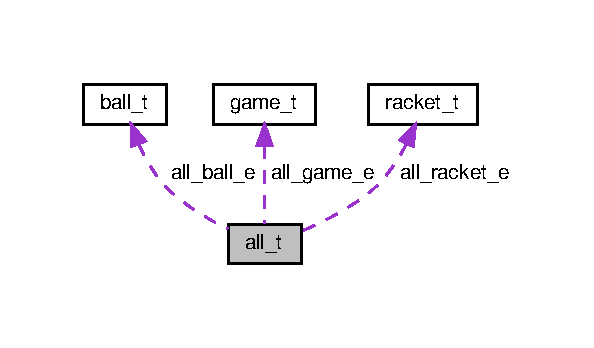
\includegraphics[width=285pt]{structall__t__coll__graph}
\end{center}
\end{figure}
\subsection*{Data Fields}
\begin{DoxyCompactItemize}
\item 
struct \hyperlink{structball__t}{ball\+\_\+t} $\ast$ \hyperlink{structall__t_a8d2313689132a052d5e697ed96c267b3}{all\+\_\+ball\+\_\+e}
\item 
struct \hyperlink{structracket__t}{racket\+\_\+t} $\ast$ \hyperlink{structall__t_a4857ea3a6650aa37b82c0e7336eaa278}{all\+\_\+racket\+\_\+e}
\item 
struct \hyperlink{structgame__t}{game\+\_\+t} $\ast$ \hyperlink{structall__t_af9c1a9096cf652aa5b37d4cc768dcd70}{all\+\_\+game\+\_\+e}
\end{DoxyCompactItemize}


\subsection{Detailed Description}
Structure containing different structures send to the different threads to run the game properly. 

Definition at line 183 of file game\+\_\+ui.\+h.



\subsection{Field Documentation}
\mbox{\Hypertarget{structall__t_a8d2313689132a052d5e697ed96c267b3}\label{structall__t_a8d2313689132a052d5e697ed96c267b3}} 
\index{all\+\_\+t@{all\+\_\+t}!all\+\_\+ball\+\_\+e@{all\+\_\+ball\+\_\+e}}
\index{all\+\_\+ball\+\_\+e@{all\+\_\+ball\+\_\+e}!all\+\_\+t@{all\+\_\+t}}
\subsubsection{\texorpdfstring{all\+\_\+ball\+\_\+e}{all\_ball\_e}}
{\footnotesize\ttfamily struct \hyperlink{structball__t}{ball\+\_\+t}$\ast$ all\+\_\+ball\+\_\+e}

structure containing a pointer to a \hyperlink{structball__t}{ball\+\_\+t} structure. 

Definition at line 185 of file game\+\_\+ui.\+h.

\mbox{\Hypertarget{structall__t_af9c1a9096cf652aa5b37d4cc768dcd70}\label{structall__t_af9c1a9096cf652aa5b37d4cc768dcd70}} 
\index{all\+\_\+t@{all\+\_\+t}!all\+\_\+game\+\_\+e@{all\+\_\+game\+\_\+e}}
\index{all\+\_\+game\+\_\+e@{all\+\_\+game\+\_\+e}!all\+\_\+t@{all\+\_\+t}}
\subsubsection{\texorpdfstring{all\+\_\+game\+\_\+e}{all\_game\_e}}
{\footnotesize\ttfamily struct \hyperlink{structgame__t}{game\+\_\+t}$\ast$ all\+\_\+game\+\_\+e}

structure containing a pointer to a \hyperlink{structgame__t}{game\+\_\+t} structure. 

Definition at line 187 of file game\+\_\+ui.\+h.

\mbox{\Hypertarget{structall__t_a4857ea3a6650aa37b82c0e7336eaa278}\label{structall__t_a4857ea3a6650aa37b82c0e7336eaa278}} 
\index{all\+\_\+t@{all\+\_\+t}!all\+\_\+racket\+\_\+e@{all\+\_\+racket\+\_\+e}}
\index{all\+\_\+racket\+\_\+e@{all\+\_\+racket\+\_\+e}!all\+\_\+t@{all\+\_\+t}}
\subsubsection{\texorpdfstring{all\+\_\+racket\+\_\+e}{all\_racket\_e}}
{\footnotesize\ttfamily struct \hyperlink{structracket__t}{racket\+\_\+t}$\ast$ all\+\_\+racket\+\_\+e}

structure containing a pointer to a \hyperlink{structracket__t}{racket\+\_\+t} structure. 

Definition at line 186 of file game\+\_\+ui.\+h.



The documentation for this struct was generated from the following file\+:\begin{DoxyCompactItemize}
\item 
/home/lafie-\/rage/\+Cours/\+L\+A1/\+P\+R\+S/\+G\+I\+T\+\_\+\+P\+R\+O\+J\+E\+T\+S/\+P\+R\+S\+\_\+\+Projet\+\_\+\+Brick\+Breaker\+\_\+\+B\+R/\hyperlink{game__ui_8h}{game\+\_\+ui.\+h}\end{DoxyCompactItemize}

\hypertarget{structball__t}{}\section{ball\+\_\+t Struct Reference}
\label{structball__t}\index{ball\+\_\+t@{ball\+\_\+t}}


Structure containing all ball information.  




{\ttfamily \#include $<$game\+\_\+ui.\+h$>$}

\subsection*{Data Fields}
\begin{DoxyCompactItemize}
\item 
int \hyperlink{structball__t_ab34f89ef94db9dd6d3a04425dd6d9c9d}{posX}
\item 
int \hyperlink{structball__t_a65ab2de052c17234c8a1db3fd3b868a9}{posY}
\item 
int \hyperlink{structball__t_ad892143587536d5edaac114b6d9b38f6}{moving}
\item 
int \hyperlink{structball__t_a349642fac223cab55f7a69e068423424}{dirX}
\item 
int \hyperlink{structball__t_aaa2cc03cc9f201b80d903336a92173a9}{dirY}
\end{DoxyCompactItemize}


\subsection{Detailed Description}
Structure containing all ball information. 

posX and posY are the X and Y coordonates of the ball on the screen moving set if the ball move or not dirX value -\/1 or 1, describe if the ball is moving to the positive or negative X coordonates dirY value -\/1 or 1, describe if the ball is moving to the positive or negative Y coordonates 

Definition at line 122 of file game\+\_\+ui.\+h.



\subsection{Field Documentation}
\mbox{\Hypertarget{structball__t_a349642fac223cab55f7a69e068423424}\label{structball__t_a349642fac223cab55f7a69e068423424}} 
\index{ball\+\_\+t@{ball\+\_\+t}!dirX@{dirX}}
\index{dirX@{dirX}!ball\+\_\+t@{ball\+\_\+t}}
\subsubsection{\texorpdfstring{dirX}{dirX}}
{\footnotesize\ttfamily int dirX}



Definition at line 127 of file game\+\_\+ui.\+h.

\mbox{\Hypertarget{structball__t_aaa2cc03cc9f201b80d903336a92173a9}\label{structball__t_aaa2cc03cc9f201b80d903336a92173a9}} 
\index{ball\+\_\+t@{ball\+\_\+t}!dirY@{dirY}}
\index{dirY@{dirY}!ball\+\_\+t@{ball\+\_\+t}}
\subsubsection{\texorpdfstring{dirY}{dirY}}
{\footnotesize\ttfamily int dirY}



Definition at line 128 of file game\+\_\+ui.\+h.

\mbox{\Hypertarget{structball__t_ad892143587536d5edaac114b6d9b38f6}\label{structball__t_ad892143587536d5edaac114b6d9b38f6}} 
\index{ball\+\_\+t@{ball\+\_\+t}!moving@{moving}}
\index{moving@{moving}!ball\+\_\+t@{ball\+\_\+t}}
\subsubsection{\texorpdfstring{moving}{moving}}
{\footnotesize\ttfamily int moving}



Definition at line 126 of file game\+\_\+ui.\+h.

\mbox{\Hypertarget{structball__t_ab34f89ef94db9dd6d3a04425dd6d9c9d}\label{structball__t_ab34f89ef94db9dd6d3a04425dd6d9c9d}} 
\index{ball\+\_\+t@{ball\+\_\+t}!posX@{posX}}
\index{posX@{posX}!ball\+\_\+t@{ball\+\_\+t}}
\subsubsection{\texorpdfstring{posX}{posX}}
{\footnotesize\ttfamily int posX}



Definition at line 124 of file game\+\_\+ui.\+h.

\mbox{\Hypertarget{structball__t_a65ab2de052c17234c8a1db3fd3b868a9}\label{structball__t_a65ab2de052c17234c8a1db3fd3b868a9}} 
\index{ball\+\_\+t@{ball\+\_\+t}!posY@{posY}}
\index{posY@{posY}!ball\+\_\+t@{ball\+\_\+t}}
\subsubsection{\texorpdfstring{posY}{posY}}
{\footnotesize\ttfamily int posY}



Definition at line 125 of file game\+\_\+ui.\+h.



The documentation for this struct was generated from the following file\+:\begin{DoxyCompactItemize}
\item 
/home/lafie-\/rage/\+Cours/\+L\+A1/\+P\+R\+S/\+G\+I\+T\+\_\+\+P\+R\+O\+J\+E\+T\+S/\+P\+R\+S\+\_\+\+Projet\+\_\+\+Brick\+Breaker\+\_\+\+B\+R/\hyperlink{game__ui_8h}{game\+\_\+ui.\+h}\end{DoxyCompactItemize}

\hypertarget{structbody}{}\section{body Struct Reference}
\label{structbody}\index{body@{body}}


{\ttfamily \#include $<$kassbriik.\+h$>$}

\subsection*{Data Fields}
\begin{DoxyCompactItemize}
\item 
pid\+\_\+t \hyperlink{structbody_ae0d46a978d5cd6707411f276ad869b9c}{pid}
\item 
char \hyperlink{structbody_ac2ac923fc89ad742c924ee62face9dc4}{message} \mbox{[}\hyperlink{kassbriik_8h_a1a92f29d280d7de1b5bc07f16dc933bf}{M\+A\+X\+\_\+\+B\+O\+D\+Y\+\_\+\+M\+S\+G\+\_\+\+S\+I\+ZE}\mbox{]}
\end{DoxyCompactItemize}


\subsection{Detailed Description}


Definition at line 239 of file kassbriik.\+h.



\subsection{Field Documentation}
\mbox{\Hypertarget{structbody_ac2ac923fc89ad742c924ee62face9dc4}\label{structbody_ac2ac923fc89ad742c924ee62face9dc4}} 
\index{body@{body}!message@{message}}
\index{message@{message}!body@{body}}
\subsubsection{\texorpdfstring{message}{message}}
{\footnotesize\ttfamily char message\mbox{[}\hyperlink{kassbriik_8h_a1a92f29d280d7de1b5bc07f16dc933bf}{M\+A\+X\+\_\+\+B\+O\+D\+Y\+\_\+\+M\+S\+G\+\_\+\+S\+I\+ZE}\mbox{]}}



Definition at line 241 of file kassbriik.\+h.

\mbox{\Hypertarget{structbody_ae0d46a978d5cd6707411f276ad869b9c}\label{structbody_ae0d46a978d5cd6707411f276ad869b9c}} 
\index{body@{body}!pid@{pid}}
\index{pid@{pid}!body@{body}}
\subsubsection{\texorpdfstring{pid}{pid}}
{\footnotesize\ttfamily pid\+\_\+t pid}



Definition at line 240 of file kassbriik.\+h.



The documentation for this struct was generated from the following file\+:\begin{DoxyCompactItemize}
\item 
/home/lafie-\/rage/\+Cours/\+L\+A1/\+P\+R\+S/\+G\+I\+T\+\_\+\+P\+R\+O\+J\+E\+T\+S/\+P\+R\+S\+\_\+\+Projet\+\_\+\+Brick\+Breaker\+\_\+\+B\+R/\hyperlink{kassbriik_8h}{kassbriik.\+h}\end{DoxyCompactItemize}

\hypertarget{structbrick__t}{}\section{brick\+\_\+t Struct Reference}
\label{structbrick__t}\index{brick\+\_\+t@{brick\+\_\+t}}


Structure containing all ball information.  




{\ttfamily \#include $<$game\+\_\+ui.\+h$>$}

\subsection*{Data Fields}
\begin{DoxyCompactItemize}
\item 
int \hyperlink{structbrick__t_ab34f89ef94db9dd6d3a04425dd6d9c9d}{posX}
\item 
int \hyperlink{structbrick__t_a65ab2de052c17234c8a1db3fd3b868a9}{posY}
\item 
int \hyperlink{structbrick__t_a2474a5474cbff19523a51eb1de01cda4}{width}
\end{DoxyCompactItemize}


\subsection{Detailed Description}
Structure containing all ball information. 

posX and posY are the X and Y coordonates of the beginning of the brick on the screen width is the width of the racket (2 by default) 

Definition at line 138 of file game\+\_\+ui.\+h.



\subsection{Field Documentation}
\mbox{\Hypertarget{structbrick__t_ab34f89ef94db9dd6d3a04425dd6d9c9d}\label{structbrick__t_ab34f89ef94db9dd6d3a04425dd6d9c9d}} 
\index{brick\+\_\+t@{brick\+\_\+t}!posX@{posX}}
\index{posX@{posX}!brick\+\_\+t@{brick\+\_\+t}}
\subsubsection{\texorpdfstring{posX}{posX}}
{\footnotesize\ttfamily int posX}



Definition at line 140 of file game\+\_\+ui.\+h.

\mbox{\Hypertarget{structbrick__t_a65ab2de052c17234c8a1db3fd3b868a9}\label{structbrick__t_a65ab2de052c17234c8a1db3fd3b868a9}} 
\index{brick\+\_\+t@{brick\+\_\+t}!posY@{posY}}
\index{posY@{posY}!brick\+\_\+t@{brick\+\_\+t}}
\subsubsection{\texorpdfstring{posY}{posY}}
{\footnotesize\ttfamily int posY}



Definition at line 141 of file game\+\_\+ui.\+h.

\mbox{\Hypertarget{structbrick__t_a2474a5474cbff19523a51eb1de01cda4}\label{structbrick__t_a2474a5474cbff19523a51eb1de01cda4}} 
\index{brick\+\_\+t@{brick\+\_\+t}!width@{width}}
\index{width@{width}!brick\+\_\+t@{brick\+\_\+t}}
\subsubsection{\texorpdfstring{width}{width}}
{\footnotesize\ttfamily int width}



Definition at line 142 of file game\+\_\+ui.\+h.



The documentation for this struct was generated from the following file\+:\begin{DoxyCompactItemize}
\item 
/home/lafie-\/rage/\+Cours/\+L\+A1/\+P\+R\+S/\+G\+I\+T\+\_\+\+P\+R\+O\+J\+E\+T\+S/\+P\+R\+S\+\_\+\+Projet\+\_\+\+Brick\+Breaker\+\_\+\+B\+R/\hyperlink{game__ui_8h}{game\+\_\+ui.\+h}\end{DoxyCompactItemize}

\hypertarget{structclient}{}\section{client Struct Reference}
\label{structclient}\index{client@{client}}


{\ttfamily \#include $<$server\+\_\+kassbriik.\+h$>$}

\subsection*{Data Fields}
\begin{DoxyCompactItemize}
\item 
int \hyperlink{structclient_af500917c052066b40cf47f96b43c607b}{pid}
\item 
char $\ast$ \hyperlink{structclient_a9b20c006bd90a09e1465fb668700e81d}{username}
\item 
int \hyperlink{structclient_aef160b7437d94056f1dc59646cd5b87d}{score}
\end{DoxyCompactItemize}


\subsection{Detailed Description}


Definition at line 35 of file server\+\_\+kassbriik.\+h.



\subsection{Field Documentation}
\mbox{\Hypertarget{structclient_af500917c052066b40cf47f96b43c607b}\label{structclient_af500917c052066b40cf47f96b43c607b}} 
\index{client@{client}!pid@{pid}}
\index{pid@{pid}!client@{client}}
\subsubsection{\texorpdfstring{pid}{pid}}
{\footnotesize\ttfamily int pid}



Definition at line 36 of file server\+\_\+kassbriik.\+h.

\mbox{\Hypertarget{structclient_aef160b7437d94056f1dc59646cd5b87d}\label{structclient_aef160b7437d94056f1dc59646cd5b87d}} 
\index{client@{client}!score@{score}}
\index{score@{score}!client@{client}}
\subsubsection{\texorpdfstring{score}{score}}
{\footnotesize\ttfamily int \hyperlink{structscore}{score}}



Definition at line 38 of file server\+\_\+kassbriik.\+h.

\mbox{\Hypertarget{structclient_a9b20c006bd90a09e1465fb668700e81d}\label{structclient_a9b20c006bd90a09e1465fb668700e81d}} 
\index{client@{client}!username@{username}}
\index{username@{username}!client@{client}}
\subsubsection{\texorpdfstring{username}{username}}
{\footnotesize\ttfamily char$\ast$ username}



Definition at line 37 of file server\+\_\+kassbriik.\+h.



The documentation for this struct was generated from the following file\+:\begin{DoxyCompactItemize}
\item 
/home/lafie-\/rage/\+Cours/\+L\+A1/\+P\+R\+S/\+G\+I\+T\+\_\+\+P\+R\+O\+J\+E\+T\+S/\+P\+R\+S\+\_\+\+Projet\+\_\+\+Brick\+Breaker\+\_\+\+B\+R/\hyperlink{server__kassbriik_8h}{server\+\_\+kassbriik.\+h}\end{DoxyCompactItemize}

\hypertarget{structclients__list}{}\section{clients\+\_\+list Struct Reference}
\label{structclients__list}\index{clients\+\_\+list@{clients\+\_\+list}}


A list of clients.  




{\ttfamily \#include $<$server\+\_\+kassbriik.\+h$>$}



Collaboration diagram for clients\+\_\+list\+:\nopagebreak
\begin{figure}[H]
\begin{center}
\leavevmode
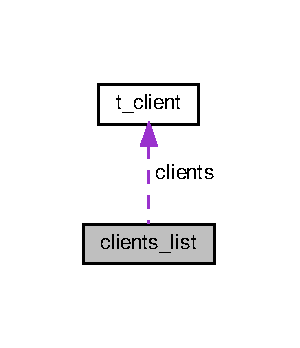
\includegraphics[width=144pt]{structclients__list__coll__graph}
\end{center}
\end{figure}
\subsection*{Data Fields}
\begin{DoxyCompactItemize}
\item 
\hyperlink{structt__client}{t\+\_\+client} $\ast$ \hyperlink{structclients__list_aebf714cf96a3647f8caa5c43c5af8ea7}{clients}
\item 
int \hyperlink{structclients__list_a439227feff9d7f55384e8780cfc2eb82}{size}
\end{DoxyCompactItemize}


\subsection{Detailed Description}
A list of clients. 

Containts the lists of the clients the server knows or want to communicate to as array of \hyperlink{structt__client}{t\+\_\+client}. Also contains is size. The clients undefined have the P\+ID -\/1. Those clients are in the client\textquotesingle{}s array from size to the length of the array. Avoid browsing the array with anything else than a for loop from 0 to size-\/1. 

Definition at line 52 of file server\+\_\+kassbriik.\+h.



\subsection{Field Documentation}
\mbox{\Hypertarget{structclients__list_aebf714cf96a3647f8caa5c43c5af8ea7}\label{structclients__list_aebf714cf96a3647f8caa5c43c5af8ea7}} 
\index{clients\+\_\+list@{clients\+\_\+list}!clients@{clients}}
\index{clients@{clients}!clients\+\_\+list@{clients\+\_\+list}}
\subsubsection{\texorpdfstring{clients}{clients}}
{\footnotesize\ttfamily \hyperlink{structt__client}{t\+\_\+client}$\ast$ clients}



Definition at line 53 of file server\+\_\+kassbriik.\+h.

\mbox{\Hypertarget{structclients__list_a439227feff9d7f55384e8780cfc2eb82}\label{structclients__list_a439227feff9d7f55384e8780cfc2eb82}} 
\index{clients\+\_\+list@{clients\+\_\+list}!size@{size}}
\index{size@{size}!clients\+\_\+list@{clients\+\_\+list}}
\subsubsection{\texorpdfstring{size}{size}}
{\footnotesize\ttfamily int size}



Definition at line 54 of file server\+\_\+kassbriik.\+h.



The documentation for this struct was generated from the following file\+:\begin{DoxyCompactItemize}
\item 
/home/lafie-\/rage/\+Cours/\+L\+A1/\+P\+R\+S/\+G\+I\+T\+\_\+\+P\+R\+O\+J\+E\+T\+S/\+P\+R\+S\+\_\+\+Projet\+\_\+\+Brick\+Breaker\+\_\+\+B\+R/\hyperlink{server__kassbriik_8h}{server\+\_\+kassbriik.\+h}\end{DoxyCompactItemize}

\hypertarget{structgame__t}{}\section{game\+\_\+t Struct Reference}
\label{structgame__t}\index{game\+\_\+t@{game\+\_\+t}}


Structure containing all the parameters important to run the game properly.  




{\ttfamily \#include $<$game\+\_\+ui.\+h$>$}

\subsection*{Data Fields}
\begin{DoxyCompactItemize}
\item 
int \hyperlink{structgame__t_aef160b7437d94056f1dc59646cd5b87d}{score}
\item 
int \hyperlink{structgame__t_abce9f5dc9c83f2639b72024fdee5d388}{end}
\item 
int \hyperlink{structgame__t_ae0c7df2c3c2bb3eb2aad3bfc63f563c3}{nb\+Ball}
\item 
int \hyperlink{structgame__t_a4e08ae0a019d63e85e4fb24954774f9d}{bricks\+Remaining}
\item 
int \hyperlink{structgame__t_a50491e00170f4adb355806cf91481163}{fromX}
\item 
int \hyperlink{structgame__t_a8da59cbd18dd05d7e77b0c9b47646fef}{toX}
\item 
int \hyperlink{structgame__t_a546e3a938f0bbf34f001c54c80a8d004}{fromY}
\item 
int \hyperlink{structgame__t_aee78eaf1a5ef0225bf8f0d146becc1ca}{turbo}
\item 
int \hyperlink{structgame__t_ae80b0201d378d6dfc9ecc3d67e3e364b}{cheat}
\end{DoxyCompactItemize}


\subsection{Detailed Description}
Structure containing all the parameters important to run the game properly. 

posX and posY are the X and Y coordonates of the ball on the screen moving set if the ball move or not dirX value -\/1 or 1, describe if the ball is moving to the positive or negative X coordonates dirY value -\/1 or 1, describe if the ball is moving to the positive or negative Y coordonates 

Definition at line 166 of file game\+\_\+ui.\+h.



\subsection{Field Documentation}
\mbox{\Hypertarget{structgame__t_a4e08ae0a019d63e85e4fb24954774f9d}\label{structgame__t_a4e08ae0a019d63e85e4fb24954774f9d}} 
\index{game\+\_\+t@{game\+\_\+t}!bricks\+Remaining@{bricks\+Remaining}}
\index{bricks\+Remaining@{bricks\+Remaining}!game\+\_\+t@{game\+\_\+t}}
\subsubsection{\texorpdfstring{bricks\+Remaining}{bricksRemaining}}
{\footnotesize\ttfamily int bricks\+Remaining}

number of bricks left on screen. 

Definition at line 171 of file game\+\_\+ui.\+h.

\mbox{\Hypertarget{structgame__t_ae80b0201d378d6dfc9ecc3d67e3e364b}\label{structgame__t_ae80b0201d378d6dfc9ecc3d67e3e364b}} 
\index{game\+\_\+t@{game\+\_\+t}!cheat@{cheat}}
\index{cheat@{cheat}!game\+\_\+t@{game\+\_\+t}}
\subsubsection{\texorpdfstring{cheat}{cheat}}
{\footnotesize\ttfamily int cheat}

activates the cheat (a huge racket taking all the screen avoiding death. 

Definition at line 176 of file game\+\_\+ui.\+h.

\mbox{\Hypertarget{structgame__t_abce9f5dc9c83f2639b72024fdee5d388}\label{structgame__t_abce9f5dc9c83f2639b72024fdee5d388}} 
\index{game\+\_\+t@{game\+\_\+t}!end@{end}}
\index{end@{end}!game\+\_\+t@{game\+\_\+t}}
\subsubsection{\texorpdfstring{end}{end}}
{\footnotesize\ttfamily int end}

if set to 1 the game ends. 

Definition at line 169 of file game\+\_\+ui.\+h.

\mbox{\Hypertarget{structgame__t_a50491e00170f4adb355806cf91481163}\label{structgame__t_a50491e00170f4adb355806cf91481163}} 
\index{game\+\_\+t@{game\+\_\+t}!fromX@{fromX}}
\index{fromX@{fromX}!game\+\_\+t@{game\+\_\+t}}
\subsubsection{\texorpdfstring{fromX}{fromX}}
{\footnotesize\ttfamily int fromX}

horizontal position from where the bricks are placed. 

Definition at line 172 of file game\+\_\+ui.\+h.

\mbox{\Hypertarget{structgame__t_a546e3a938f0bbf34f001c54c80a8d004}\label{structgame__t_a546e3a938f0bbf34f001c54c80a8d004}} 
\index{game\+\_\+t@{game\+\_\+t}!fromY@{fromY}}
\index{fromY@{fromY}!game\+\_\+t@{game\+\_\+t}}
\subsubsection{\texorpdfstring{fromY}{fromY}}
{\footnotesize\ttfamily int fromY}

vertical position from where the bricks are placed. 

Definition at line 174 of file game\+\_\+ui.\+h.

\mbox{\Hypertarget{structgame__t_ae0c7df2c3c2bb3eb2aad3bfc63f563c3}\label{structgame__t_ae0c7df2c3c2bb3eb2aad3bfc63f563c3}} 
\index{game\+\_\+t@{game\+\_\+t}!nb\+Ball@{nb\+Ball}}
\index{nb\+Ball@{nb\+Ball}!game\+\_\+t@{game\+\_\+t}}
\subsubsection{\texorpdfstring{nb\+Ball}{nbBall}}
{\footnotesize\ttfamily int nb\+Ball}

number of ball (or lives) remaining before the game if over. 

Definition at line 170 of file game\+\_\+ui.\+h.

\mbox{\Hypertarget{structgame__t_aef160b7437d94056f1dc59646cd5b87d}\label{structgame__t_aef160b7437d94056f1dc59646cd5b87d}} 
\index{game\+\_\+t@{game\+\_\+t}!score@{score}}
\index{score@{score}!game\+\_\+t@{game\+\_\+t}}
\subsubsection{\texorpdfstring{score}{score}}
{\footnotesize\ttfamily int \hyperlink{structscore}{score}}

variable used to store the score of the player. 

Definition at line 168 of file game\+\_\+ui.\+h.

\mbox{\Hypertarget{structgame__t_a8da59cbd18dd05d7e77b0c9b47646fef}\label{structgame__t_a8da59cbd18dd05d7e77b0c9b47646fef}} 
\index{game\+\_\+t@{game\+\_\+t}!toX@{toX}}
\index{toX@{toX}!game\+\_\+t@{game\+\_\+t}}
\subsubsection{\texorpdfstring{toX}{toX}}
{\footnotesize\ttfamily int toX}

horizontal position until which brick are placed. 

Definition at line 173 of file game\+\_\+ui.\+h.

\mbox{\Hypertarget{structgame__t_aee78eaf1a5ef0225bf8f0d146becc1ca}\label{structgame__t_aee78eaf1a5ef0225bf8f0d146becc1ca}} 
\index{game\+\_\+t@{game\+\_\+t}!turbo@{turbo}}
\index{turbo@{turbo}!game\+\_\+t@{game\+\_\+t}}
\subsubsection{\texorpdfstring{turbo}{turbo}}
{\footnotesize\ttfamily int turbo}

acts on game speed (the bigger it is the faster the game runs. 

Definition at line 175 of file game\+\_\+ui.\+h.



The documentation for this struct was generated from the following file\+:\begin{DoxyCompactItemize}
\item 
/home/lafie-\/rage/\+Cours/\+L\+A1/\+P\+R\+S/\+G\+I\+T\+\_\+\+P\+R\+O\+J\+E\+T\+S/\+P\+R\+S\+\_\+\+Projet\+\_\+\+Brick\+Breaker\+\_\+\+B\+R/\hyperlink{game__ui_8h}{game\+\_\+ui.\+h}\end{DoxyCompactItemize}

\hypertarget{structracket__t}{}\section{racket\+\_\+t Struct Reference}
\label{structracket__t}\index{racket\+\_\+t@{racket\+\_\+t}}


Structure containing all racket information.  




{\ttfamily \#include $<$game\+\_\+ui.\+h$>$}

\subsection*{Data Fields}
\begin{DoxyCompactItemize}
\item 
int \hyperlink{structracket__t_ab34f89ef94db9dd6d3a04425dd6d9c9d}{posX}
\item 
int \hyperlink{structracket__t_a65ab2de052c17234c8a1db3fd3b868a9}{posY}
\end{DoxyCompactItemize}


\subsection{Detailed Description}
Structure containing all racket information. 

posX and posY are the X and Y coordonates of the racket on the screen 

Definition at line 151 of file game\+\_\+ui.\+h.



\subsection{Field Documentation}
\mbox{\Hypertarget{structracket__t_ab34f89ef94db9dd6d3a04425dd6d9c9d}\label{structracket__t_ab34f89ef94db9dd6d3a04425dd6d9c9d}} 
\index{racket\+\_\+t@{racket\+\_\+t}!posX@{posX}}
\index{posX@{posX}!racket\+\_\+t@{racket\+\_\+t}}
\subsubsection{\texorpdfstring{posX}{posX}}
{\footnotesize\ttfamily int posX}



Definition at line 153 of file game\+\_\+ui.\+h.

\mbox{\Hypertarget{structracket__t_a65ab2de052c17234c8a1db3fd3b868a9}\label{structracket__t_a65ab2de052c17234c8a1db3fd3b868a9}} 
\index{racket\+\_\+t@{racket\+\_\+t}!posY@{posY}}
\index{posY@{posY}!racket\+\_\+t@{racket\+\_\+t}}
\subsubsection{\texorpdfstring{posY}{posY}}
{\footnotesize\ttfamily int posY}



Definition at line 154 of file game\+\_\+ui.\+h.



The documentation for this struct was generated from the following file\+:\begin{DoxyCompactItemize}
\item 
/home/lafie-\/rage/\+Cours/\+L\+A1/\+P\+R\+S/\+G\+I\+T\+\_\+\+P\+R\+O\+J\+E\+T\+S/\+P\+R\+S\+\_\+\+Projet\+\_\+\+Brick\+Breaker\+\_\+\+B\+R/\hyperlink{game__ui_8h}{game\+\_\+ui.\+h}\end{DoxyCompactItemize}

\hypertarget{structrequest}{}\section{request Struct Reference}
\label{structrequest}\index{request@{request}}


{\ttfamily \#include $<$kassbriik.\+h$>$}



Collaboration diagram for request\+:\nopagebreak
\begin{figure}[H]
\begin{center}
\leavevmode
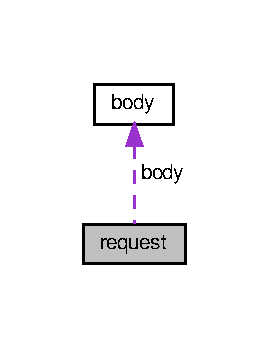
\includegraphics[width=130pt]{structrequest__coll__graph}
\end{center}
\end{figure}
\subsection*{Data Fields}
\begin{DoxyCompactItemize}
\item 
long \hyperlink{structrequest_a6a83a8677f7c78fd146859325e08209a}{type}
\item 
\hyperlink{structt__body}{t\+\_\+body} \hyperlink{structrequest_ab79c1a13ebd161031c617d5f313e3cae}{body}
\end{DoxyCompactItemize}


\subsection{Detailed Description}


Definition at line 252 of file kassbriik.\+h.



\subsection{Field Documentation}
\mbox{\Hypertarget{structrequest_ab79c1a13ebd161031c617d5f313e3cae}\label{structrequest_ab79c1a13ebd161031c617d5f313e3cae}} 
\index{request@{request}!body@{body}}
\index{body@{body}!request@{request}}
\subsubsection{\texorpdfstring{body}{body}}
{\footnotesize\ttfamily \hyperlink{structt__body}{t\+\_\+body} \hyperlink{structbody}{body}}



Definition at line 254 of file kassbriik.\+h.

\mbox{\Hypertarget{structrequest_a6a83a8677f7c78fd146859325e08209a}\label{structrequest_a6a83a8677f7c78fd146859325e08209a}} 
\index{request@{request}!type@{type}}
\index{type@{type}!request@{request}}
\subsubsection{\texorpdfstring{type}{type}}
{\footnotesize\ttfamily long type}



Definition at line 253 of file kassbriik.\+h.



The documentation for this struct was generated from the following file\+:\begin{DoxyCompactItemize}
\item 
/home/lafie-\/rage/\+Cours/\+L\+A1/\+P\+R\+S/\+G\+I\+T\+\_\+\+P\+R\+O\+J\+E\+T\+S/\+P\+R\+S\+\_\+\+Projet\+\_\+\+Brick\+Breaker\+\_\+\+B\+R/\hyperlink{kassbriik_8h}{kassbriik.\+h}\end{DoxyCompactItemize}

\hypertarget{structscore}{}\section{score Struct Reference}
\label{structscore}\index{score@{score}}


{\ttfamily \#include $<$kassbriik.\+h$>$}

\subsection*{Data Fields}
\begin{DoxyCompactItemize}
\item 
int \hyperlink{structscore_aef160b7437d94056f1dc59646cd5b87d}{score}
\item 
char \hyperlink{structscore_a3dae4259c0ca612dbb2b1ac5f21def5d}{username} \mbox{[}50\mbox{]}
\end{DoxyCompactItemize}


\subsection{Detailed Description}


Definition at line 93 of file kassbriik.\+h.



\subsection{Field Documentation}
\mbox{\Hypertarget{structscore_aef160b7437d94056f1dc59646cd5b87d}\label{structscore_aef160b7437d94056f1dc59646cd5b87d}} 
\index{score@{score}!score@{score}}
\index{score@{score}!score@{score}}
\subsubsection{\texorpdfstring{score}{score}}
{\footnotesize\ttfamily int \hyperlink{structscore}{score}}



Definition at line 94 of file kassbriik.\+h.

\mbox{\Hypertarget{structscore_a3dae4259c0ca612dbb2b1ac5f21def5d}\label{structscore_a3dae4259c0ca612dbb2b1ac5f21def5d}} 
\index{score@{score}!username@{username}}
\index{username@{username}!score@{score}}
\subsubsection{\texorpdfstring{username}{username}}
{\footnotesize\ttfamily char username\mbox{[}50\mbox{]}}



Definition at line 95 of file kassbriik.\+h.



The documentation for this struct was generated from the following file\+:\begin{DoxyCompactItemize}
\item 
/home/lafie-\/rage/\+Cours/\+L\+A1/\+P\+R\+S/\+G\+I\+T\+\_\+\+P\+R\+O\+J\+E\+T\+S/\+P\+R\+S\+\_\+\+Projet\+\_\+\+Brick\+Breaker\+\_\+\+B\+R/\hyperlink{kassbriik_8h}{kassbriik.\+h}\end{DoxyCompactItemize}

\hypertarget{structscores__list}{}\section{scores\+\_\+list Struct Reference}
\label{structscores__list}\index{scores\+\_\+list@{scores\+\_\+list}}


{\ttfamily \#include $<$kassbriik.\+h$>$}



Collaboration diagram for scores\+\_\+list\+:\nopagebreak
\begin{figure}[H]
\begin{center}
\leavevmode
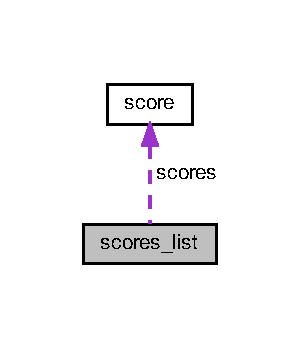
\includegraphics[width=145pt]{structscores__list__coll__graph}
\end{center}
\end{figure}
\subsection*{Data Fields}
\begin{DoxyCompactItemize}
\item 
\hyperlink{structt__score}{t\+\_\+score} \hyperlink{structscores__list_a419b845c86c29189d87e70fd893a024d}{scores} \mbox{[}\hyperlink{kassbriik_8h_a0a8f91f93d75a07f0ae45077db45b3eb}{M\+A\+X\+\_\+\+C\+L\+I\+E\+N\+TS}\mbox{]}
\item 
int \hyperlink{structscores__list_a439227feff9d7f55384e8780cfc2eb82}{size}
\end{DoxyCompactItemize}


\subsection{Detailed Description}


Definition at line 105 of file kassbriik.\+h.



\subsection{Field Documentation}
\mbox{\Hypertarget{structscores__list_a419b845c86c29189d87e70fd893a024d}\label{structscores__list_a419b845c86c29189d87e70fd893a024d}} 
\index{scores\+\_\+list@{scores\+\_\+list}!scores@{scores}}
\index{scores@{scores}!scores\+\_\+list@{scores\+\_\+list}}
\subsubsection{\texorpdfstring{scores}{scores}}
{\footnotesize\ttfamily \hyperlink{structt__score}{t\+\_\+score} scores\mbox{[}\hyperlink{kassbriik_8h_a0a8f91f93d75a07f0ae45077db45b3eb}{M\+A\+X\+\_\+\+C\+L\+I\+E\+N\+TS}\mbox{]}}



Definition at line 106 of file kassbriik.\+h.

\mbox{\Hypertarget{structscores__list_a439227feff9d7f55384e8780cfc2eb82}\label{structscores__list_a439227feff9d7f55384e8780cfc2eb82}} 
\index{scores\+\_\+list@{scores\+\_\+list}!size@{size}}
\index{size@{size}!scores\+\_\+list@{scores\+\_\+list}}
\subsubsection{\texorpdfstring{size}{size}}
{\footnotesize\ttfamily int size}



Definition at line 107 of file kassbriik.\+h.



The documentation for this struct was generated from the following file\+:\begin{DoxyCompactItemize}
\item 
/home/lafie-\/rage/\+Cours/\+L\+A1/\+P\+R\+S/\+G\+I\+T\+\_\+\+P\+R\+O\+J\+E\+T\+S/\+P\+R\+S\+\_\+\+Projet\+\_\+\+Brick\+Breaker\+\_\+\+B\+R/\hyperlink{kassbriik_8h}{kassbriik.\+h}\end{DoxyCompactItemize}

\hypertarget{structt__body}{}\section{t\+\_\+body Struct Reference}
\label{structt__body}\index{t\+\_\+body@{t\+\_\+body}}


Body of a \hyperlink{structt__request}{t\+\_\+request}.  




{\ttfamily \#include $<$kassbriik.\+h$>$}



\subsection{Detailed Description}
Body of a \hyperlink{structt__request}{t\+\_\+request}. 

Containts the message to send and the source pid. 

The documentation for this struct was generated from the following file\+:\begin{DoxyCompactItemize}
\item 
/home/lafie-\/rage/\+Cours/\+L\+A1/\+P\+R\+S/\+G\+I\+T\+\_\+\+P\+R\+O\+J\+E\+T\+S/\+P\+R\+S\+\_\+\+Projet\+\_\+\+Brick\+Breaker\+\_\+\+B\+R/\hyperlink{kassbriik_8h}{kassbriik.\+h}\end{DoxyCompactItemize}

\hypertarget{structt__client}{}\section{t\+\_\+client Struct Reference}
\label{structt__client}\index{t\+\_\+client@{t\+\_\+client}}


Structure of a client view by the server.  




{\ttfamily \#include $<$server\+\_\+kassbriik.\+h$>$}



\subsection{Detailed Description}
Structure of a client view by the server. 

/file \hyperlink{server__kassbriik_8h}{server\+\_\+kassbriik.\+h} /author Corentin D\+E\+S\+T\+R\+EZ \& Valentin G\+U\+I\+B\+E\+R\+T\+E\+AU /date 09 Apr 2021 /brief Header of the server\textquotesingle{}s library

This library containts the definition of some useful values, functions and structures that are used by the server.

This library also include thoose \+: -\/$>$ sys/types.\+h

Contains the P\+ID of the client \& the username of the player. 

The documentation for this struct was generated from the following file\+:\begin{DoxyCompactItemize}
\item 
/home/lafie-\/rage/\+Cours/\+L\+A1/\+P\+R\+S/\+G\+I\+T\+\_\+\+P\+R\+O\+J\+E\+T\+S/\+P\+R\+S\+\_\+\+Projet\+\_\+\+Brick\+Breaker\+\_\+\+B\+R/\hyperlink{server__kassbriik_8h}{server\+\_\+kassbriik.\+h}\end{DoxyCompactItemize}

\hypertarget{structt__request}{}\section{t\+\_\+request Struct Reference}
\label{structt__request}\index{t\+\_\+request@{t\+\_\+request}}


Request send via the message queue.  




{\ttfamily \#include $<$kassbriik.\+h$>$}



\subsection{Detailed Description}
Request send via the message queue. 

t\+\_\+reuest are the messages send via the message queue. It\textquotesingle{}s composed of the body (as \hyperlink{structt__body}{t\+\_\+body}) and the type of request. 

The documentation for this struct was generated from the following file\+:\begin{DoxyCompactItemize}
\item 
/home/lafie-\/rage/\+Cours/\+L\+A1/\+P\+R\+S/\+G\+I\+T\+\_\+\+P\+R\+O\+J\+E\+T\+S/\+P\+R\+S\+\_\+\+Projet\+\_\+\+Brick\+Breaker\+\_\+\+B\+R/\hyperlink{kassbriik_8h}{kassbriik.\+h}\end{DoxyCompactItemize}

\hypertarget{structt__score}{}\section{t\+\_\+score Struct Reference}
\label{structt__score}\index{t\+\_\+score@{t\+\_\+score}}


Structure of a score view by the client.  




{\ttfamily \#include $<$kassbriik.\+h$>$}



\subsection{Detailed Description}
Structure of a score view by the client. 

Contains the username of the player and its score. 

The documentation for this struct was generated from the following file\+:\begin{DoxyCompactItemize}
\item 
/home/lafie-\/rage/\+Cours/\+L\+A1/\+P\+R\+S/\+G\+I\+T\+\_\+\+P\+R\+O\+J\+E\+T\+S/\+P\+R\+S\+\_\+\+Projet\+\_\+\+Brick\+Breaker\+\_\+\+B\+R/\hyperlink{kassbriik_8h}{kassbriik.\+h}\end{DoxyCompactItemize}

\hypertarget{structt__scores__list}{}\section{t\+\_\+scores\+\_\+list Struct Reference}
\label{structt__scores__list}\index{t\+\_\+scores\+\_\+list@{t\+\_\+scores\+\_\+list}}


A list of \hyperlink{structt__score}{t\+\_\+score} knonwing its size.  




{\ttfamily \#include $<$kassbriik.\+h$>$}



\subsection{Detailed Description}
A list of \hyperlink{structt__score}{t\+\_\+score} knonwing its size. 

Contains a list of scores and the size of the list. 

The documentation for this struct was generated from the following file\+:\begin{DoxyCompactItemize}
\item 
/home/lafie-\/rage/\+Cours/\+L\+A1/\+P\+R\+S/\+G\+I\+T\+\_\+\+P\+R\+O\+J\+E\+T\+S/\+P\+R\+S\+\_\+\+Projet\+\_\+\+Brick\+Breaker\+\_\+\+B\+R/\hyperlink{kassbriik_8h}{kassbriik.\+h}\end{DoxyCompactItemize}

\chapter{File Documentation}
\hypertarget{client_8c}{}\section{/home/lafie-\/rage/\+Cours/\+L\+A1/\+P\+R\+S/\+G\+I\+T\+\_\+\+P\+R\+O\+J\+E\+T\+S/\+P\+R\+S\+\_\+\+Projet\+\_\+\+Brick\+Breaker\+\_\+\+B\+R/client.c File Reference}
\label{client_8c}\index{/home/lafie-\/rage/\+Cours/\+L\+A1/\+P\+R\+S/\+G\+I\+T\+\_\+\+P\+R\+O\+J\+E\+T\+S/\+P\+R\+S\+\_\+\+Projet\+\_\+\+Brick\+Breaker\+\_\+\+B\+R/client.\+c@{/home/lafie-\/rage/\+Cours/\+L\+A1/\+P\+R\+S/\+G\+I\+T\+\_\+\+P\+R\+O\+J\+E\+T\+S/\+P\+R\+S\+\_\+\+Projet\+\_\+\+Brick\+Breaker\+\_\+\+B\+R/client.\+c}}
{\ttfamily \#include $<$stdio.\+h$>$}\newline
{\ttfamily \#include $<$stdlib.\+h$>$}\newline
{\ttfamily \#include $<$string.\+h$>$}\newline
{\ttfamily \#include $<$unistd.\+h$>$}\newline
{\ttfamily \#include \char`\"{}kassbriik.\+h\char`\"{}}\newline
{\ttfamily \#include \char`\"{}game\+\_\+ui.\+h\char`\"{}}\newline
Include dependency graph for client.\+c\+:\nopagebreak
\begin{figure}[H]
\begin{center}
\leavevmode
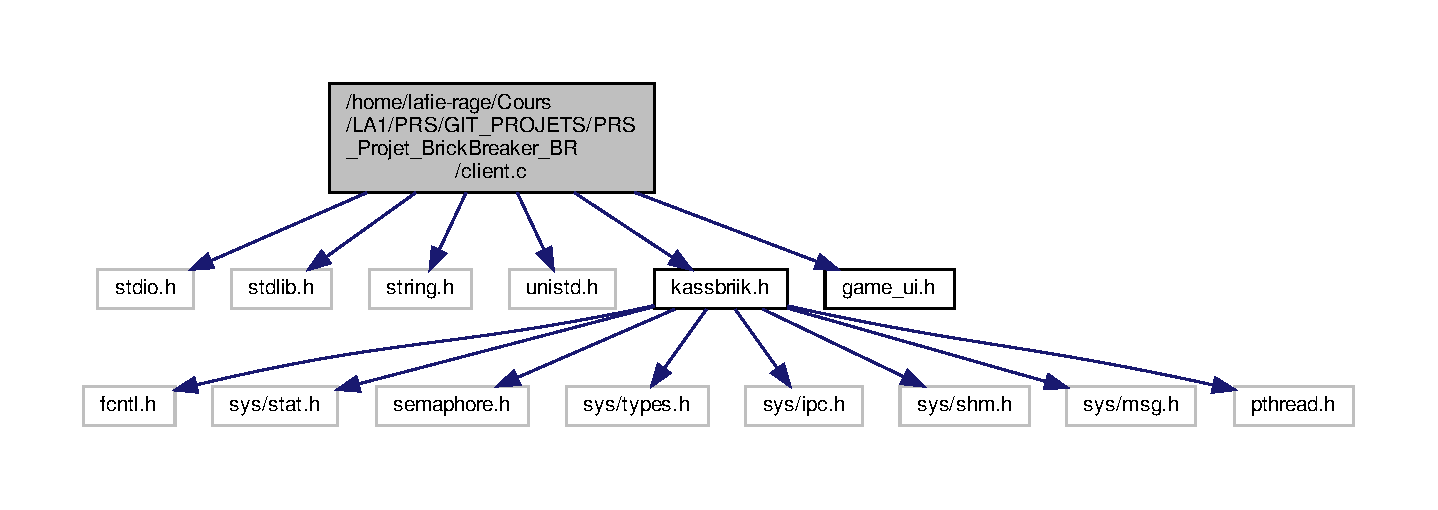
\includegraphics[width=350pt]{client_8c__incl}
\end{center}
\end{figure}
\subsection*{Functions}
\begin{DoxyCompactItemize}
\item 
void \hyperlink{client_8c_aef4ea26c670e5d4a9f6a60c844bdd4f6}{init\+Server\+Connection} (int $\ast$msg\+Id, int $\ast$server\+Pid, char $\ast$username)
\item 
void \hyperlink{client_8c_a325494eb677c39bc868b6aa8e2ac3335}{connect\+To\+Server} (int msg\+Id, char $\ast$username)
\item 
void \hyperlink{client_8c_a6dc6d4c6635b0f45c5fb1ab00af29168}{ask\+Server\+To\+Launch\+The\+Game} (int msg\+Id)
\begin{DoxyCompactList}\small\item\em Wait for the server to launch the game, then start it. \end{DoxyCompactList}\item 
void \hyperlink{client_8c_ad1dc38571963869004d74ccd5e657646}{notify\+Server\+That\+Game\+Has\+Started} (int msg\+Id)
\begin{DoxyCompactList}\small\item\em Notify the server that the client has started the game. \end{DoxyCompactList}\item 
void \hyperlink{client_8c_a297c894356d29912f8d2df16aff30c29}{send\+Score} (int msg\+Id, int \hyperlink{structscore}{score})
\begin{DoxyCompactList}\small\item\em Send the score of the player to the server. \end{DoxyCompactList}\item 
void \hyperlink{client_8c_a5f632b8eb71f198600be67f236590bce}{open\+Shm\+And\+Semaphore} (int $\ast$shm\+Id, struct shmid\+\_\+ds $\ast$shm\+Buffer, \hyperlink{structt__scores__list}{t\+\_\+scores\+\_\+list} $\ast$$\ast$shm\+Ptr, sem\+\_\+t $\ast$sem\+Id)
\begin{DoxyCompactList}\small\item\em Open the shm and its semaphore. \end{DoxyCompactList}\item 
void \hyperlink{client_8c_a33b5072cad34944ee1ac35bcf5c83a5a}{retrieve\+Scores} (int msg\+Id, \hyperlink{structt__scores__list}{t\+\_\+scores\+\_\+list} $\ast$scores)
\begin{DoxyCompactList}\small\item\em Retrieve the score of each players from the server. \end{DoxyCompactList}\item 
void \hyperlink{client_8c_a0097956ffe3311ddcede01803cd665cc}{print\+Final\+Rank} (int msg\+Id, \hyperlink{structt__scores__list}{t\+\_\+scores\+\_\+list} scores)
\begin{DoxyCompactList}\small\item\em Print the scores. \end{DoxyCompactList}\item 
int \hyperlink{client_8c_a0ddf1224851353fc92bfbff6f499fa97}{main} (int argc, char $\ast$argv\mbox{[}$\,$\mbox{]})
\end{DoxyCompactItemize}


\subsection{Function Documentation}
\mbox{\Hypertarget{client_8c_a6dc6d4c6635b0f45c5fb1ab00af29168}\label{client_8c_a6dc6d4c6635b0f45c5fb1ab00af29168}} 
\index{client.\+c@{client.\+c}!ask\+Server\+To\+Launch\+The\+Game@{ask\+Server\+To\+Launch\+The\+Game}}
\index{ask\+Server\+To\+Launch\+The\+Game@{ask\+Server\+To\+Launch\+The\+Game}!client.\+c@{client.\+c}}
\subsubsection{\texorpdfstring{ask\+Server\+To\+Launch\+The\+Game()}{askServerToLaunchTheGame()}}
{\footnotesize\ttfamily void ask\+Server\+To\+Launch\+The\+Game (\begin{DoxyParamCaption}\item[{int}]{msg\+Id }\end{DoxyParamCaption})}



Wait for the server to launch the game, then start it. 

Await for the server\textquotesingle{}s message to start the game, reply to him and then launch it. Display message during process.


\begin{DoxyParams}{Parameters}
{\em msg\+Id} & Pointer where their is the file descriptor of the message queue to use to send the message. \\
\hline
\end{DoxyParams}


Definition at line 167 of file client.\+c.

\mbox{\Hypertarget{client_8c_a325494eb677c39bc868b6aa8e2ac3335}\label{client_8c_a325494eb677c39bc868b6aa8e2ac3335}} 
\index{client.\+c@{client.\+c}!connect\+To\+Server@{connect\+To\+Server}}
\index{connect\+To\+Server@{connect\+To\+Server}!client.\+c@{client.\+c}}
\subsubsection{\texorpdfstring{connect\+To\+Server()}{connectToServer()}}
{\footnotesize\ttfamily void connect\+To\+Server (\begin{DoxyParamCaption}\item[{int}]{msg\+Id,  }\item[{char $\ast$}]{username }\end{DoxyParamCaption})}



Definition at line 158 of file client.\+c.

\mbox{\Hypertarget{client_8c_aef4ea26c670e5d4a9f6a60c844bdd4f6}\label{client_8c_aef4ea26c670e5d4a9f6a60c844bdd4f6}} 
\index{client.\+c@{client.\+c}!init\+Server\+Connection@{init\+Server\+Connection}}
\index{init\+Server\+Connection@{init\+Server\+Connection}!client.\+c@{client.\+c}}
\subsubsection{\texorpdfstring{init\+Server\+Connection()}{initServerConnection()}}
{\footnotesize\ttfamily void init\+Server\+Connection (\begin{DoxyParamCaption}\item[{int $\ast$}]{msg\+Id,  }\item[{int $\ast$}]{server\+Pid,  }\item[{char $\ast$}]{username }\end{DoxyParamCaption})}



Definition at line 145 of file client.\+c.

\mbox{\Hypertarget{client_8c_a0ddf1224851353fc92bfbff6f499fa97}\label{client_8c_a0ddf1224851353fc92bfbff6f499fa97}} 
\index{client.\+c@{client.\+c}!main@{main}}
\index{main@{main}!client.\+c@{client.\+c}}
\subsubsection{\texorpdfstring{main()}{main()}}
{\footnotesize\ttfamily int main (\begin{DoxyParamCaption}\item[{int}]{argc,  }\item[{char $\ast$}]{argv\mbox{[}$\,$\mbox{]} }\end{DoxyParamCaption})}



Definition at line 124 of file client.\+c.

\mbox{\Hypertarget{client_8c_ad1dc38571963869004d74ccd5e657646}\label{client_8c_ad1dc38571963869004d74ccd5e657646}} 
\index{client.\+c@{client.\+c}!notify\+Server\+That\+Game\+Has\+Started@{notify\+Server\+That\+Game\+Has\+Started}}
\index{notify\+Server\+That\+Game\+Has\+Started@{notify\+Server\+That\+Game\+Has\+Started}!client.\+c@{client.\+c}}
\subsubsection{\texorpdfstring{notify\+Server\+That\+Game\+Has\+Started()}{notifyServerThatGameHasStarted()}}
{\footnotesize\ttfamily void notify\+Server\+That\+Game\+Has\+Started (\begin{DoxyParamCaption}\item[{int}]{msg\+Id }\end{DoxyParamCaption})}



Notify the server that the client has started the game. 

Notify the server that the client has started the game via message queue. Display message during process.


\begin{DoxyParams}{Parameters}
{\em msg\+Id} & Pointer where their is the file descriptor of the message queue to use to send the message. \\
\hline
\end{DoxyParams}


Definition at line 175 of file client.\+c.

\mbox{\Hypertarget{client_8c_a5f632b8eb71f198600be67f236590bce}\label{client_8c_a5f632b8eb71f198600be67f236590bce}} 
\index{client.\+c@{client.\+c}!open\+Shm\+And\+Semaphore@{open\+Shm\+And\+Semaphore}}
\index{open\+Shm\+And\+Semaphore@{open\+Shm\+And\+Semaphore}!client.\+c@{client.\+c}}
\subsubsection{\texorpdfstring{open\+Shm\+And\+Semaphore()}{openShmAndSemaphore()}}
{\footnotesize\ttfamily void open\+Shm\+And\+Semaphore (\begin{DoxyParamCaption}\item[{int $\ast$}]{shm\+Id,  }\item[{struct shmid\+\_\+ds $\ast$}]{shm\+Buffer,  }\item[{\hyperlink{structt__scores__list}{t\+\_\+scores\+\_\+list} $\ast$$\ast$}]{shm\+Ptr,  }\item[{sem\+\_\+t $\ast$}]{sem\+Id }\end{DoxyParamCaption})}



Open the shm and its semaphore. 

Send the score of the player to the server via message queue. Display message during process.


\begin{DoxyParams}{Parameters}
{\em msg\+Id} & Pointer where their is the file descriptor of the message queue to use to send the message. \\
\hline
{\em score} & The score of the player. \\
\hline
{\em shm\+Ptr} & The pointer to the shm. \\
\hline
{\em sem\+Id} & The semaphore\textquotesingle{}s id. \\
\hline
\end{DoxyParams}


Definition at line 198 of file client.\+c.

\mbox{\Hypertarget{client_8c_a0097956ffe3311ddcede01803cd665cc}\label{client_8c_a0097956ffe3311ddcede01803cd665cc}} 
\index{client.\+c@{client.\+c}!print\+Final\+Rank@{print\+Final\+Rank}}
\index{print\+Final\+Rank@{print\+Final\+Rank}!client.\+c@{client.\+c}}
\subsubsection{\texorpdfstring{print\+Final\+Rank()}{printFinalRank()}}
{\footnotesize\ttfamily void print\+Final\+Rank (\begin{DoxyParamCaption}\item[{int}]{msg\+Id,  }\item[{\hyperlink{structt__scores__list}{t\+\_\+scores\+\_\+list}}]{scores }\end{DoxyParamCaption})}



Print the scores. 

Print the scores to the player and say who is the winner.


\begin{DoxyItemize}
\item 
\begin{DoxyParams}{Parameters}
{\em msg\+Id} & Pointer where their is the file descriptor of the message queue to use to send the message. \\
\hline
{\em scores} & The list of scores of each players. \\
\hline
\end{DoxyParams}

\end{DoxyItemize}

Definition at line 234 of file client.\+c.

\mbox{\Hypertarget{client_8c_a33b5072cad34944ee1ac35bcf5c83a5a}\label{client_8c_a33b5072cad34944ee1ac35bcf5c83a5a}} 
\index{client.\+c@{client.\+c}!retrieve\+Scores@{retrieve\+Scores}}
\index{retrieve\+Scores@{retrieve\+Scores}!client.\+c@{client.\+c}}
\subsubsection{\texorpdfstring{retrieve\+Scores()}{retrieveScores()}}
{\footnotesize\ttfamily void retrieve\+Scores (\begin{DoxyParamCaption}\item[{int}]{smh\+Id,  }\item[{\hyperlink{structt__scores__list}{t\+\_\+scores\+\_\+list} $\ast$}]{scores }\end{DoxyParamCaption})}



Retrieve the score of each players from the server. 

Retieve the socre of each player from the server via message queue. Display message during process.


\begin{DoxyParams}{Parameters}
{\em msg\+Id} & Pointer where their is the file descriptor of the message queue to use to send the message. \\
\hline
{\em scores} & The list of scores. \\
\hline
\end{DoxyParams}


Definition at line 211 of file client.\+c.

\mbox{\Hypertarget{client_8c_a297c894356d29912f8d2df16aff30c29}\label{client_8c_a297c894356d29912f8d2df16aff30c29}} 
\index{client.\+c@{client.\+c}!send\+Score@{send\+Score}}
\index{send\+Score@{send\+Score}!client.\+c@{client.\+c}}
\subsubsection{\texorpdfstring{send\+Score()}{sendScore()}}
{\footnotesize\ttfamily void send\+Score (\begin{DoxyParamCaption}\item[{int}]{msg\+Id,  }\item[{int}]{score }\end{DoxyParamCaption})}



Send the score of the player to the server. 

Send the score of the player to the server via message queue. Display message during process.


\begin{DoxyParams}{Parameters}
{\em msg\+Id} & Pointer where their is the file descriptor of the message queue to use to send the message. \\
\hline
{\em score} & The score of the player. \\
\hline
\end{DoxyParams}


Definition at line 184 of file client.\+c.


\hypertarget{game__ui_8c}{}\section{/home/lafie-\/rage/\+Cours/\+L\+A1/\+P\+R\+S/\+G\+I\+T\+\_\+\+P\+R\+O\+J\+E\+T\+S/\+P\+R\+S\+\_\+\+Projet\+\_\+\+Brick\+Breaker\+\_\+\+B\+R/game\+\_\+ui.c File Reference}
\label{game__ui_8c}\index{/home/lafie-\/rage/\+Cours/\+L\+A1/\+P\+R\+S/\+G\+I\+T\+\_\+\+P\+R\+O\+J\+E\+T\+S/\+P\+R\+S\+\_\+\+Projet\+\_\+\+Brick\+Breaker\+\_\+\+B\+R/game\+\_\+ui.\+c@{/home/lafie-\/rage/\+Cours/\+L\+A1/\+P\+R\+S/\+G\+I\+T\+\_\+\+P\+R\+O\+J\+E\+T\+S/\+P\+R\+S\+\_\+\+Projet\+\_\+\+Brick\+Breaker\+\_\+\+B\+R/game\+\_\+ui.\+c}}
{\ttfamily \#include $<$stdio.\+h$>$}\newline
{\ttfamily \#include $<$string.\+h$>$}\newline
{\ttfamily \#include $<$stdlib.\+h$>$}\newline
{\ttfamily \#include $<$unistd.\+h$>$}\newline
{\ttfamily \#include $<$pthread.\+h$>$}\newline
{\ttfamily \#include $<$termios.\+h$>$}\newline
{\ttfamily \#include $<$semaphore.\+h$>$}\newline
{\ttfamily \#include $<$sys/select.\+h$>$}\newline
{\ttfamily \#include \char`\"{}game\+\_\+ui.\+h\char`\"{}}\newline
Include dependency graph for game\+\_\+ui.\+c\+:\nopagebreak
\begin{figure}[H]
\begin{center}
\leavevmode
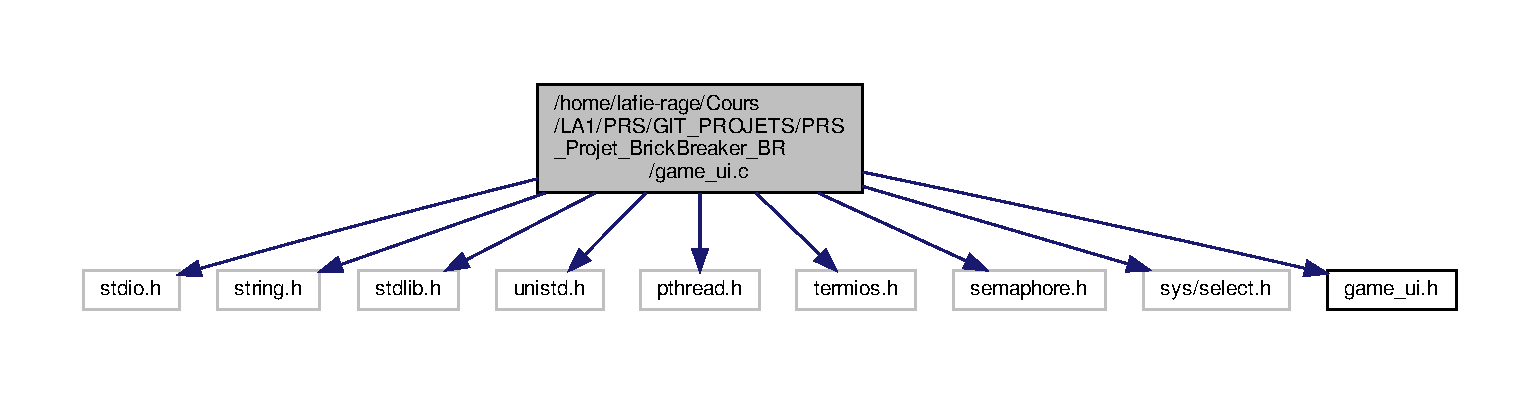
\includegraphics[width=350pt]{game__ui_8c__incl}
\end{center}
\end{figure}
\subsection*{Functions}
\begin{DoxyCompactItemize}
\item 
int \hyperlink{game__ui_8c_a43d17e02a89ed4b1459b42aa86901f51}{start\+Game\+UI} ()
\item 
void \hyperlink{game__ui_8c_a4f6f385b448f3bfe07f14a810e8fae8c}{place\+Element\+From} (int x, int y, int w, int h, char e)
\begin{DoxyCompactList}\small\item\em place every element possible in the game to set the base screen (or debug purposes). \end{DoxyCompactList}\item 
void \hyperlink{game__ui_8c_aad32b015d56f990ecefdc5a467d34ebb}{place\+Huge\+Racket} ()
\begin{DoxyCompactList}\small\item\em place a huge racket avoiding death. \end{DoxyCompactList}\item 
void \hyperlink{game__ui_8c_a1b646a9989d9764d785de9a332962944}{remove\+Huge\+Racket} ()
\begin{DoxyCompactList}\small\item\em remove the huge racket avoiding death. \end{DoxyCompactList}\item 
void \hyperlink{game__ui_8c_ae8d0d97bd4f5aa117715206251fbf053}{place\+Brick} (int x, int y, \hyperlink{structgame__t}{game\+\_\+t} $\ast$game\+\_\+e)
\begin{DoxyCompactList}\small\item\em place one brick beginning at the x and y coordonates indicated. \end{DoxyCompactList}\item 
void \hyperlink{game__ui_8c_aeec2b4731d6382c72e268c2fdb2b3466}{destroy\+Brick} (int x, int y, \hyperlink{structgame__t}{game\+\_\+t} $\ast$game\+\_\+e)
\begin{DoxyCompactList}\small\item\em destroy the brick begining at the x and y coordonates indicated. \end{DoxyCompactList}\item 
void \hyperlink{game__ui_8c_a183b7fa713e49fcf385bdc14b870c388}{place\+Bricks} (int x, int y, int mx, int my, \hyperlink{structgame__t}{game\+\_\+t} $\ast$game\+\_\+e)
\begin{DoxyCompactList}\small\item\em place brick beginning at the x and y coordonates indicated to the mx and my coordonates indicated. \end{DoxyCompactList}\item 
void \hyperlink{game__ui_8c_ac77d5caeeb189a0491e5874625211c4c}{move\+Racket} (\hyperlink{structracket__t}{racket\+\_\+t} $\ast$racket\+\_\+e, char c)
\begin{DoxyCompactList}\small\item\em move the racket accordingly to the input of the user q for left d for right. \end{DoxyCompactList}\item 
void \hyperlink{game__ui_8c_ad7fd45cf7c5d225bf8077fbe401c9ab7}{collision} (\hyperlink{structball__t}{ball\+\_\+t} $\ast$ball\+\_\+e, \hyperlink{structgame__t}{game\+\_\+t} $\ast$game\+\_\+e)
\begin{DoxyCompactList}\small\item\em deals with all the collisions in the game. \end{DoxyCompactList}\item 
void \hyperlink{game__ui_8c_a45d1e11ad1048311b06473924acf8ca6}{move\+B\+A\+LL} (\hyperlink{structball__t}{ball\+\_\+t} $\ast$ball\+\_\+e, \hyperlink{structgame__t}{game\+\_\+t} $\ast$game\+\_\+e)
\begin{DoxyCompactList}\small\item\em move the ball after the collision treatment. \end{DoxyCompactList}\item 
void \hyperlink{game__ui_8c_a153f6816fbb1f4e0132d2fd3a8dd4057}{draw\+Screen} (\hyperlink{structgame__t}{game\+\_\+t} $\ast$game\+\_\+e)
\begin{DoxyCompactList}\small\item\em draws the caracter on the user screen accordingly to the array \char`\"{}screen\char`\"{} content. \end{DoxyCompactList}\item 
void $\ast$ \hyperlink{game__ui_8c_a330b973683c1d1f6830619af51b47335}{f\+Display} (void $\ast$arg)
\begin{DoxyCompactList}\small\item\em function used in a thread to deal with the display the game on the user\textquotesingle{}s screen. \end{DoxyCompactList}\item 
int \hyperlink{game__ui_8c_ad5451da499ab9d3907da8dd7060ab677}{kbhit} ()
\item 
int \hyperlink{game__ui_8c_a160f6d2893bb6b89ab3ad5d863c20e3d}{getch} ()
\item 
void $\ast$ \hyperlink{game__ui_8c_aa9c5404a0d538b8ab80211cb0d71363f}{f\+Input} (void $\ast$arg)
\begin{DoxyCompactList}\small\item\em function used in a thread to deal with the input of the game. \end{DoxyCompactList}\end{DoxyCompactItemize}
\subsection*{Variables}
\begin{DoxyCompactItemize}
\item 
char \hyperlink{game__ui_8c_a1f8be2a692d10738ddc1bbd4856c9d33}{screen} \mbox{[}\hyperlink{game__ui_8h_a321cf56a944d4adca0ea6dfbd2577030}{W\+I\+D\+T\+H\+\_\+\+M\+AX}\mbox{]}\mbox{[}\hyperlink{game__ui_8h_a3f1ca00f1b8d2d99f50894e87f6f62b2}{H\+E\+I\+G\+H\+T\+\_\+\+M\+AX}\mbox{]}
\item 
\hyperlink{structbrick__t}{brick\+\_\+t} $\ast$ \hyperlink{game__ui_8c_a1565f4f4190f2c4191975a1f586f8629}{bricks}
\end{DoxyCompactItemize}


\subsection{Function Documentation}
\mbox{\Hypertarget{game__ui_8c_ad7fd45cf7c5d225bf8077fbe401c9ab7}\label{game__ui_8c_ad7fd45cf7c5d225bf8077fbe401c9ab7}} 
\index{game\+\_\+ui.\+c@{game\+\_\+ui.\+c}!collision@{collision}}
\index{collision@{collision}!game\+\_\+ui.\+c@{game\+\_\+ui.\+c}}
\subsubsection{\texorpdfstring{collision()}{collision()}}
{\footnotesize\ttfamily void collision (\begin{DoxyParamCaption}\item[{\hyperlink{structball__t}{ball\+\_\+t} $\ast$}]{ball\+\_\+e,  }\item[{\hyperlink{structgame__t}{game\+\_\+t} $\ast$}]{game\+\_\+e }\end{DoxyParamCaption})}



deals with all the collisions in the game. 


\begin{DoxyParams}{Parameters}
{\em game\+\_\+e} & structure containing all game info. \\
\hline
{\em ball\+\_\+e} & structure containing all ball info. \\
\hline
\end{DoxyParams}
this section deals with the ball hiting th bottom of the screen

heart of the collision detection

$<$ potential detection on the pair component of the brick hit. 

Definition at line 269 of file game\+\_\+ui.\+c.

\mbox{\Hypertarget{game__ui_8c_aeec2b4731d6382c72e268c2fdb2b3466}\label{game__ui_8c_aeec2b4731d6382c72e268c2fdb2b3466}} 
\index{game\+\_\+ui.\+c@{game\+\_\+ui.\+c}!destroy\+Brick@{destroy\+Brick}}
\index{destroy\+Brick@{destroy\+Brick}!game\+\_\+ui.\+c@{game\+\_\+ui.\+c}}
\subsubsection{\texorpdfstring{destroy\+Brick()}{destroyBrick()}}
{\footnotesize\ttfamily void destroy\+Brick (\begin{DoxyParamCaption}\item[{int}]{x,  }\item[{int}]{y,  }\item[{\hyperlink{structgame__t}{game\+\_\+t} $\ast$}]{game\+\_\+e }\end{DoxyParamCaption})}



destroy the brick begining at the x and y coordonates indicated. 


\begin{DoxyParams}{Parameters}
{\em x} & base horizontal position of the brick. \\
\hline
{\em y} & base vertical position of the brick. \\
\hline
{\em game\+\_\+e} & structure containing all game info. \\
\hline
\end{DoxyParams}


Definition at line 205 of file game\+\_\+ui.\+c.

\mbox{\Hypertarget{game__ui_8c_a153f6816fbb1f4e0132d2fd3a8dd4057}\label{game__ui_8c_a153f6816fbb1f4e0132d2fd3a8dd4057}} 
\index{game\+\_\+ui.\+c@{game\+\_\+ui.\+c}!draw\+Screen@{draw\+Screen}}
\index{draw\+Screen@{draw\+Screen}!game\+\_\+ui.\+c@{game\+\_\+ui.\+c}}
\subsubsection{\texorpdfstring{draw\+Screen()}{drawScreen()}}
{\footnotesize\ttfamily void draw\+Screen (\begin{DoxyParamCaption}\item[{\hyperlink{structgame__t}{game\+\_\+t} $\ast$}]{game\+\_\+e }\end{DoxyParamCaption})}



draws the caracter on the user screen accordingly to the array \char`\"{}screen\char`\"{} content. 


\begin{DoxyParams}{Parameters}
{\em game\+\_\+e} & structure containing all game info. \\
\hline
\end{DoxyParams}
draws the bottom of the screen with different information for the user.

Definition at line 388 of file game\+\_\+ui.\+c.

\mbox{\Hypertarget{game__ui_8c_a330b973683c1d1f6830619af51b47335}\label{game__ui_8c_a330b973683c1d1f6830619af51b47335}} 
\index{game\+\_\+ui.\+c@{game\+\_\+ui.\+c}!f\+Display@{f\+Display}}
\index{f\+Display@{f\+Display}!game\+\_\+ui.\+c@{game\+\_\+ui.\+c}}
\subsubsection{\texorpdfstring{f\+Display()}{fDisplay()}}
{\footnotesize\ttfamily void $\ast$ f\+Display (\begin{DoxyParamCaption}\item[{void $\ast$}]{arg }\end{DoxyParamCaption})}



function used in a thread to deal with the display the game on the user\textquotesingle{}s screen. 

I couldn\textquotesingle{}t find the original site for kbhit and getch definition but they can be found on \+: \href{https://forum.df2.ru/lofiversion/index.php/t16583-50.html}{\tt https\+://forum.\+df2.\+ru/lofiversion/index.\+php/t16583-\/50.\+html} 

Definition at line 435 of file game\+\_\+ui.\+c.

\mbox{\Hypertarget{game__ui_8c_aa9c5404a0d538b8ab80211cb0d71363f}\label{game__ui_8c_aa9c5404a0d538b8ab80211cb0d71363f}} 
\index{game\+\_\+ui.\+c@{game\+\_\+ui.\+c}!f\+Input@{f\+Input}}
\index{f\+Input@{f\+Input}!game\+\_\+ui.\+c@{game\+\_\+ui.\+c}}
\subsubsection{\texorpdfstring{f\+Input()}{fInput()}}
{\footnotesize\ttfamily void $\ast$ f\+Input (\begin{DoxyParamCaption}\item[{void $\ast$}]{arg }\end{DoxyParamCaption})}



function used in a thread to deal with the input of the game. 



Definition at line 465 of file game\+\_\+ui.\+c.

\mbox{\Hypertarget{game__ui_8c_a160f6d2893bb6b89ab3ad5d863c20e3d}\label{game__ui_8c_a160f6d2893bb6b89ab3ad5d863c20e3d}} 
\index{game\+\_\+ui.\+c@{game\+\_\+ui.\+c}!getch@{getch}}
\index{getch@{getch}!game\+\_\+ui.\+c@{game\+\_\+ui.\+c}}
\subsubsection{\texorpdfstring{getch()}{getch()}}
{\footnotesize\ttfamily int getch (\begin{DoxyParamCaption}{ }\end{DoxyParamCaption})}

I couldn\textquotesingle{}t find the original site for kbhit and getch definition but they can be found on \+: \href{https://forum.df2.ru/lofiversion/index.php/t16583-50.html}{\tt https\+://forum.\+df2.\+ru/lofiversion/index.\+php/t16583-\/50.\+html} 

Definition at line 454 of file game\+\_\+ui.\+c.

\mbox{\Hypertarget{game__ui_8c_ad5451da499ab9d3907da8dd7060ab677}\label{game__ui_8c_ad5451da499ab9d3907da8dd7060ab677}} 
\index{game\+\_\+ui.\+c@{game\+\_\+ui.\+c}!kbhit@{kbhit}}
\index{kbhit@{kbhit}!game\+\_\+ui.\+c@{game\+\_\+ui.\+c}}
\subsubsection{\texorpdfstring{kbhit()}{kbhit()}}
{\footnotesize\ttfamily int kbhit (\begin{DoxyParamCaption}{ }\end{DoxyParamCaption})}



Definition at line 446 of file game\+\_\+ui.\+c.

\mbox{\Hypertarget{game__ui_8c_a45d1e11ad1048311b06473924acf8ca6}\label{game__ui_8c_a45d1e11ad1048311b06473924acf8ca6}} 
\index{game\+\_\+ui.\+c@{game\+\_\+ui.\+c}!move\+B\+A\+LL@{move\+B\+A\+LL}}
\index{move\+B\+A\+LL@{move\+B\+A\+LL}!game\+\_\+ui.\+c@{game\+\_\+ui.\+c}}
\subsubsection{\texorpdfstring{move\+B\+A\+L\+L()}{moveBALL()}}
{\footnotesize\ttfamily void move\+B\+A\+LL (\begin{DoxyParamCaption}\item[{\hyperlink{structball__t}{ball\+\_\+t} $\ast$}]{ball\+\_\+e,  }\item[{\hyperlink{structgame__t}{game\+\_\+t} $\ast$}]{game\+\_\+e }\end{DoxyParamCaption})}



move the ball after the collision treatment. 


\begin{DoxyParams}{Parameters}
{\em game\+\_\+e} & structure containing all game info. \\
\hline
{\em ball\+\_\+e} & structure containing all ball info. \\
\hline
\end{DoxyParams}
$<$ empty the last position of the ball on the screen.

$<$ draws the ball on it\textquotesingle{}s new position on the screen. 

Definition at line 376 of file game\+\_\+ui.\+c.

\mbox{\Hypertarget{game__ui_8c_ac77d5caeeb189a0491e5874625211c4c}\label{game__ui_8c_ac77d5caeeb189a0491e5874625211c4c}} 
\index{game\+\_\+ui.\+c@{game\+\_\+ui.\+c}!move\+Racket@{move\+Racket}}
\index{move\+Racket@{move\+Racket}!game\+\_\+ui.\+c@{game\+\_\+ui.\+c}}
\subsubsection{\texorpdfstring{move\+Racket()}{moveRacket()}}
{\footnotesize\ttfamily void move\+Racket (\begin{DoxyParamCaption}\item[{\hyperlink{structracket__t}{racket\+\_\+t} $\ast$}]{racket\+\_\+e,  }\item[{char}]{c }\end{DoxyParamCaption})}



move the racket accordingly to the input of the user q for left d for right. 


\begin{DoxyParams}{Parameters}
{\em ball\+\_\+e} & structure containing all ball info. \\
\hline
{\em c} & input received from the keyboard. \\
\hline
\end{DoxyParams}


Definition at line 236 of file game\+\_\+ui.\+c.

\mbox{\Hypertarget{game__ui_8c_ae8d0d97bd4f5aa117715206251fbf053}\label{game__ui_8c_ae8d0d97bd4f5aa117715206251fbf053}} 
\index{game\+\_\+ui.\+c@{game\+\_\+ui.\+c}!place\+Brick@{place\+Brick}}
\index{place\+Brick@{place\+Brick}!game\+\_\+ui.\+c@{game\+\_\+ui.\+c}}
\subsubsection{\texorpdfstring{place\+Brick()}{placeBrick()}}
{\footnotesize\ttfamily void place\+Brick (\begin{DoxyParamCaption}\item[{int}]{x,  }\item[{int}]{y,  }\item[{\hyperlink{structgame__t}{game\+\_\+t} $\ast$}]{game\+\_\+e }\end{DoxyParamCaption})}



place one brick beginning at the x and y coordonates indicated. 


\begin{DoxyParams}{Parameters}
{\em x} & base horizontal position of the brick. \\
\hline
{\em y} & base vertical position of the brick. \\
\hline
{\em game\+\_\+e} & structure containing all game info. \\
\hline
\end{DoxyParams}


Definition at line 193 of file game\+\_\+ui.\+c.

\mbox{\Hypertarget{game__ui_8c_a183b7fa713e49fcf385bdc14b870c388}\label{game__ui_8c_a183b7fa713e49fcf385bdc14b870c388}} 
\index{game\+\_\+ui.\+c@{game\+\_\+ui.\+c}!place\+Bricks@{place\+Bricks}}
\index{place\+Bricks@{place\+Bricks}!game\+\_\+ui.\+c@{game\+\_\+ui.\+c}}
\subsubsection{\texorpdfstring{place\+Bricks()}{placeBricks()}}
{\footnotesize\ttfamily void place\+Bricks (\begin{DoxyParamCaption}\item[{int}]{x,  }\item[{int}]{y,  }\item[{int}]{mx,  }\item[{int}]{my,  }\item[{\hyperlink{structgame__t}{game\+\_\+t} $\ast$}]{game\+\_\+e }\end{DoxyParamCaption})}



place brick beginning at the x and y coordonates indicated to the mx and my coordonates indicated. 


\begin{DoxyParams}{Parameters}
{\em x} & base horizontal position. \\
\hline
{\em y} & base vertical position. \\
\hline
{\em mx} & end horizontal position. \\
\hline
{\em my} & end vertical position. \\
\hline
{\em game\+\_\+e} & structure containing all game info. \\
\hline
\end{DoxyParams}


Definition at line 219 of file game\+\_\+ui.\+c.

\mbox{\Hypertarget{game__ui_8c_a4f6f385b448f3bfe07f14a810e8fae8c}\label{game__ui_8c_a4f6f385b448f3bfe07f14a810e8fae8c}} 
\index{game\+\_\+ui.\+c@{game\+\_\+ui.\+c}!place\+Element\+From@{place\+Element\+From}}
\index{place\+Element\+From@{place\+Element\+From}!game\+\_\+ui.\+c@{game\+\_\+ui.\+c}}
\subsubsection{\texorpdfstring{place\+Element\+From()}{placeElementFrom()}}
{\footnotesize\ttfamily void place\+Element\+From (\begin{DoxyParamCaption}\item[{int}]{x,  }\item[{int}]{y,  }\item[{int}]{w,  }\item[{int}]{h,  }\item[{char}]{e }\end{DoxyParamCaption})}



place every element possible in the game to set the base screen (or debug purposes). 


\begin{DoxyParams}{Parameters}
{\em x} & base horizontal position. \\
\hline
{\em y} & base vertical position. \\
\hline
{\em w} & end horizontal position. \\
\hline
{\em h} & end vertical position. \\
\hline
\end{DoxyParams}


Definition at line 140 of file game\+\_\+ui.\+c.

\mbox{\Hypertarget{game__ui_8c_aad32b015d56f990ecefdc5a467d34ebb}\label{game__ui_8c_aad32b015d56f990ecefdc5a467d34ebb}} 
\index{game\+\_\+ui.\+c@{game\+\_\+ui.\+c}!place\+Huge\+Racket@{place\+Huge\+Racket}}
\index{place\+Huge\+Racket@{place\+Huge\+Racket}!game\+\_\+ui.\+c@{game\+\_\+ui.\+c}}
\subsubsection{\texorpdfstring{place\+Huge\+Racket()}{placeHugeRacket()}}
{\footnotesize\ttfamily void place\+Huge\+Racket (\begin{DoxyParamCaption}{ }\end{DoxyParamCaption})}



place a huge racket avoiding death. 



Definition at line 175 of file game\+\_\+ui.\+c.

\mbox{\Hypertarget{game__ui_8c_a1b646a9989d9764d785de9a332962944}\label{game__ui_8c_a1b646a9989d9764d785de9a332962944}} 
\index{game\+\_\+ui.\+c@{game\+\_\+ui.\+c}!remove\+Huge\+Racket@{remove\+Huge\+Racket}}
\index{remove\+Huge\+Racket@{remove\+Huge\+Racket}!game\+\_\+ui.\+c@{game\+\_\+ui.\+c}}
\subsubsection{\texorpdfstring{remove\+Huge\+Racket()}{removeHugeRacket()}}
{\footnotesize\ttfamily void remove\+Huge\+Racket (\begin{DoxyParamCaption}{ }\end{DoxyParamCaption})}



remove the huge racket avoiding death. 



Definition at line 184 of file game\+\_\+ui.\+c.

\mbox{\Hypertarget{game__ui_8c_a43d17e02a89ed4b1459b42aa86901f51}\label{game__ui_8c_a43d17e02a89ed4b1459b42aa86901f51}} 
\index{game\+\_\+ui.\+c@{game\+\_\+ui.\+c}!start\+Game\+UI@{start\+Game\+UI}}
\index{start\+Game\+UI@{start\+Game\+UI}!game\+\_\+ui.\+c@{game\+\_\+ui.\+c}}
\subsubsection{\texorpdfstring{start\+Game\+U\+I()}{startGameUI()}}
{\footnotesize\ttfamily int start\+Game\+UI (\begin{DoxyParamCaption}{ }\end{DoxyParamCaption})}

\textbackslash{} Brief Start the game\textquotesingle{}s UI

Start the game UI to let the player play the game after that the server ask it. Then return the player\textquotesingle{}s score.

\begin{DoxyReturn}{Returns}
The player\textquotesingle{}s score at the end of the game. 
\end{DoxyReturn}
part used to initialise the game with its parameters.

$<$ fill the screen with void.

$<$ place the roof.

$<$ place the walls.

$<$ place the floor.

$<$ place the bricks.

place the racket and set its parameters.

$<$ used to display on the screen the racket.

initialisation of the struct ball.

initialisation of the struct containing all oher stucts.

creation of the two threads dealing with the inputs and the display of the game.

$<$ use system call to make terminal send all keystrokes directly to stdin without waiting for return presses.

end of the part used to initialise the game with its parameters.

ball position update routine

part to set back the default terminal configuration

$<$ set back echo mode.

$<$ set the changed setting to the terminal.

$<$ set back of the tty to cooked (waiting for return to validate input).

closure of the threads and end of the program.

Definition at line 32 of file game\+\_\+ui.\+c.



\subsection{Variable Documentation}
\mbox{\Hypertarget{game__ui_8c_a1565f4f4190f2c4191975a1f586f8629}\label{game__ui_8c_a1565f4f4190f2c4191975a1f586f8629}} 
\index{game\+\_\+ui.\+c@{game\+\_\+ui.\+c}!bricks@{bricks}}
\index{bricks@{bricks}!game\+\_\+ui.\+c@{game\+\_\+ui.\+c}}
\subsubsection{\texorpdfstring{bricks}{bricks}}
{\footnotesize\ttfamily \hyperlink{structbrick__t}{brick\+\_\+t}$\ast$ bricks}

array all the bricks on the screen. 

Definition at line 30 of file game\+\_\+ui.\+c.

\mbox{\Hypertarget{game__ui_8c_a1f8be2a692d10738ddc1bbd4856c9d33}\label{game__ui_8c_a1f8be2a692d10738ddc1bbd4856c9d33}} 
\index{game\+\_\+ui.\+c@{game\+\_\+ui.\+c}!screen@{screen}}
\index{screen@{screen}!game\+\_\+ui.\+c@{game\+\_\+ui.\+c}}
\subsubsection{\texorpdfstring{screen}{screen}}
{\footnotesize\ttfamily char screen\mbox{[}\hyperlink{game__ui_8h_a321cf56a944d4adca0ea6dfbd2577030}{W\+I\+D\+T\+H\+\_\+\+M\+AX}\mbox{]}\mbox{[}\hyperlink{game__ui_8h_a3f1ca00f1b8d2d99f50894e87f6f62b2}{H\+E\+I\+G\+H\+T\+\_\+\+M\+AX}\mbox{]}}



Definition at line 28 of file game\+\_\+ui.\+c.


\hypertarget{game__ui_8h}{}\section{/home/lafie-\/rage/\+Cours/\+L\+A1/\+P\+R\+S/\+G\+I\+T\+\_\+\+P\+R\+O\+J\+E\+T\+S/\+P\+R\+S\+\_\+\+Projet\+\_\+\+Brick\+Breaker\+\_\+\+B\+R/game\+\_\+ui.h File Reference}
\label{game__ui_8h}\index{/home/lafie-\/rage/\+Cours/\+L\+A1/\+P\+R\+S/\+G\+I\+T\+\_\+\+P\+R\+O\+J\+E\+T\+S/\+P\+R\+S\+\_\+\+Projet\+\_\+\+Brick\+Breaker\+\_\+\+B\+R/game\+\_\+ui.\+h@{/home/lafie-\/rage/\+Cours/\+L\+A1/\+P\+R\+S/\+G\+I\+T\+\_\+\+P\+R\+O\+J\+E\+T\+S/\+P\+R\+S\+\_\+\+Projet\+\_\+\+Brick\+Breaker\+\_\+\+B\+R/game\+\_\+ui.\+h}}
This graph shows which files directly or indirectly include this file\+:\nopagebreak
\begin{figure}[H]
\begin{center}
\leavevmode
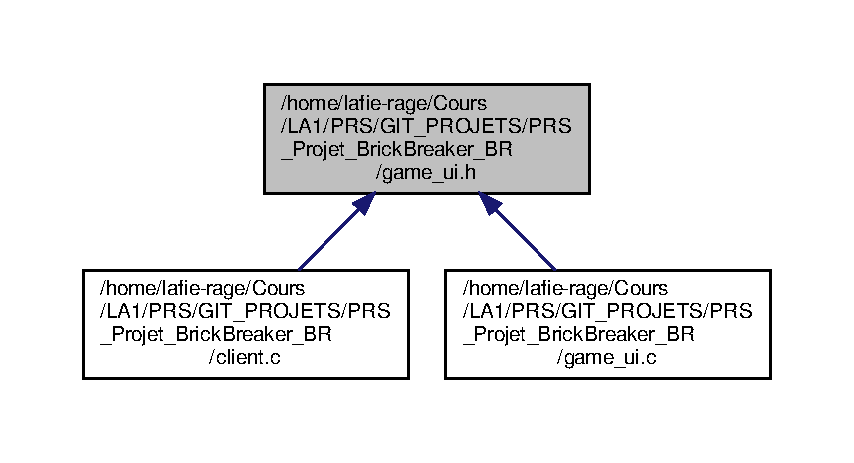
\includegraphics[width=350pt]{game__ui_8h__dep__incl}
\end{center}
\end{figure}
\subsection*{Data Structures}
\begin{DoxyCompactItemize}
\item 
struct \hyperlink{structball__t}{ball\+\_\+t}
\begin{DoxyCompactList}\small\item\em Structure containing all ball information. \end{DoxyCompactList}\item 
struct \hyperlink{structbrick__t}{brick\+\_\+t}
\begin{DoxyCompactList}\small\item\em Structure containing all ball information. \end{DoxyCompactList}\item 
struct \hyperlink{structracket__t}{racket\+\_\+t}
\begin{DoxyCompactList}\small\item\em Structure containing all racket information. \end{DoxyCompactList}\item 
struct \hyperlink{structgame__t}{game\+\_\+t}
\begin{DoxyCompactList}\small\item\em Structure containing all the parameters important to run the game properly. \end{DoxyCompactList}\item 
struct \hyperlink{structall__t}{all\+\_\+t}
\begin{DoxyCompactList}\small\item\em Structure containing different structures send to the different threads to run the game properly. \end{DoxyCompactList}\end{DoxyCompactItemize}
\subsection*{Macros}
\begin{DoxyCompactItemize}
\item 
\#define \hyperlink{game__ui_8h_a7645a891a19088e6fc698d38435dd4c9}{G\+A\+M\+E\+\_\+\+S\+P\+E\+ED}~128000
\begin{DoxyCompactList}\small\item\em number of milli seconds between each ball movement (32000=30fps) 128 000 recommended for playable experience \end{DoxyCompactList}\item 
\#define \hyperlink{game__ui_8h_a321cf56a944d4adca0ea6dfbd2577030}{W\+I\+D\+T\+H\+\_\+\+M\+AX}~80
\begin{DoxyCompactList}\small\item\em Screen width. \end{DoxyCompactList}\item 
\#define \hyperlink{game__ui_8h_a3f1ca00f1b8d2d99f50894e87f6f62b2}{H\+E\+I\+G\+H\+T\+\_\+\+M\+AX}~20
\begin{DoxyCompactList}\small\item\em Screen height. \end{DoxyCompactList}\item 
\#define \hyperlink{game__ui_8h_a15bd1a7109dfbc9c82dc540bfd227608}{B\+R\+I\+C\+K\+\_\+\+W\+I\+D\+TH}~2
\begin{DoxyCompactList}\small\item\em Brick width. \end{DoxyCompactList}\item 
\#define \hyperlink{game__ui_8h_a2d4a03fef4d0624eb9ebe9d805f029c6}{S\+I\+D\+E\+\_\+\+W\+A\+L\+L\+\_\+\+W\+I\+D\+TH}~2
\begin{DoxyCompactList}\small\item\em side walls width from screen border \end{DoxyCompactList}\item 
\#define \hyperlink{game__ui_8h_abc6585dd5bc21fbc6eac76da1d8dc52f}{U\+P\+P\+E\+R\+\_\+\+W\+A\+L\+L\+\_\+\+H\+E\+I\+G\+HT}~3
\begin{DoxyCompactList}\small\item\em upper wall height from screen border \end{DoxyCompactList}\item 
\#define \hyperlink{game__ui_8h_a9888a4d1b687327ac992eb0724613fdb}{R\+A\+C\+K\+E\+T\+\_\+\+S\+I\+ZE}~7
\begin{DoxyCompactList}\small\item\em size of the racket \end{DoxyCompactList}\item 
\#define \hyperlink{game__ui_8h_a2b7cf2a3641be7b89138615764d60ba3}{E\+M\+P\+TY}~\textquotesingle{} \textquotesingle{}
\begin{DoxyCompactList}\small\item\em caracter used for void \end{DoxyCompactList}\item 
\#define \hyperlink{game__ui_8h_ac749b87dd5d843e4add3eb8e8a130f62}{W\+A\+LL}~\textquotesingle{}W\textquotesingle{}
\begin{DoxyCompactList}\small\item\em caracter used for walls \end{DoxyCompactList}\item 
\#define \hyperlink{game__ui_8h_ac4da397dc617c6f9de08af1b87ee0d92}{B\+R\+I\+CK}~\textquotesingle{}B\textquotesingle{}
\begin{DoxyCompactList}\small\item\em caracter used for bricks \end{DoxyCompactList}\item 
\#define \hyperlink{game__ui_8h_a56509f77cfe531ba3c43f75ad9fde5f0}{B\+A\+LL}~\textquotesingle{}o\textquotesingle{}
\begin{DoxyCompactList}\small\item\em caracter used for the ball \end{DoxyCompactList}\item 
\#define \hyperlink{game__ui_8h_a043ffd71200288b5d6edb70add345b85}{R\+A\+C\+K\+ET}~\textquotesingle{}$\sim$\textquotesingle{}
\begin{DoxyCompactList}\small\item\em caracter used for the racket \end{DoxyCompactList}\item 
\#define \hyperlink{game__ui_8h_ac2c579c7b450b319336bfdf232434d89}{E\+R\+R\+O\+R\+\_\+C}~\textquotesingle{}R\textquotesingle{}
\begin{DoxyCompactList}\small\item\em caracter used for the error caracter \end{DoxyCompactList}\item 
\#define \hyperlink{game__ui_8h_a8d4a77fae1d4a62581ff791bdd176cb6}{E\+\_\+\+T\+R\+I\+G\+G\+ER}~\textquotesingle{}E\textquotesingle{}
\begin{DoxyCompactList}\small\item\em caracter used to trigger the death of a ball \end{DoxyCompactList}\end{DoxyCompactItemize}
\subsection*{Typedefs}
\begin{DoxyCompactItemize}
\item 
typedef struct \hyperlink{structball__t}{ball\+\_\+t} \hyperlink{game__ui_8h_aabbf9c15a4333ea4aded041521eba978}{ball\+\_\+t}
\item 
typedef struct \hyperlink{structbrick__t}{brick\+\_\+t} \hyperlink{game__ui_8h_a39e2f330766800b2b0a06bf13827e78c}{brick\+\_\+t}
\item 
typedef struct \hyperlink{structracket__t}{racket\+\_\+t} \hyperlink{game__ui_8h_a0da373d6cc54d371b0e7b4a9e1586e00}{racket\+\_\+t}
\item 
typedef struct \hyperlink{structgame__t}{game\+\_\+t} \hyperlink{game__ui_8h_a4b4ce1f3b7db5fed333b7457623ece8c}{game\+\_\+t}
\item 
typedef struct \hyperlink{structall__t}{all\+\_\+t} \hyperlink{game__ui_8h_a0c86d7f44a84c8d396174dca2c605f19}{all\+\_\+t}
\end{DoxyCompactItemize}
\subsection*{Functions}
\begin{DoxyCompactItemize}
\item 
void \hyperlink{game__ui_8h_a4f6f385b448f3bfe07f14a810e8fae8c}{place\+Element\+From} (int x, int y, int w, int h, char e)
\begin{DoxyCompactList}\small\item\em place every element possible in the game to set the base screen (or debug purposes). \end{DoxyCompactList}\item 
void \hyperlink{game__ui_8h_aad32b015d56f990ecefdc5a467d34ebb}{place\+Huge\+Racket} ()
\begin{DoxyCompactList}\small\item\em place a huge racket avoiding death. \end{DoxyCompactList}\item 
void \hyperlink{game__ui_8h_a1b646a9989d9764d785de9a332962944}{remove\+Huge\+Racket} ()
\begin{DoxyCompactList}\small\item\em remove the huge racket avoiding death. \end{DoxyCompactList}\item 
void \hyperlink{game__ui_8h_ae8d0d97bd4f5aa117715206251fbf053}{place\+Brick} (int x, int y, \hyperlink{structgame__t}{game\+\_\+t} $\ast$game\+\_\+e)
\begin{DoxyCompactList}\small\item\em place one brick beginning at the x and y coordonates indicated. \end{DoxyCompactList}\item 
void \hyperlink{game__ui_8h_aeec2b4731d6382c72e268c2fdb2b3466}{destroy\+Brick} (int x, int y, \hyperlink{structgame__t}{game\+\_\+t} $\ast$game\+\_\+e)
\begin{DoxyCompactList}\small\item\em destroy the brick begining at the x and y coordonates indicated. \end{DoxyCompactList}\item 
void \hyperlink{game__ui_8h_a183b7fa713e49fcf385bdc14b870c388}{place\+Bricks} (int x, int y, int mx, int my, \hyperlink{structgame__t}{game\+\_\+t} $\ast$game\+\_\+e)
\begin{DoxyCompactList}\small\item\em place brick beginning at the x and y coordonates indicated to the mx and my coordonates indicated. \end{DoxyCompactList}\item 
void \hyperlink{game__ui_8h_ac77d5caeeb189a0491e5874625211c4c}{move\+Racket} (\hyperlink{structracket__t}{racket\+\_\+t} $\ast$racket\+\_\+e, char c)
\begin{DoxyCompactList}\small\item\em move the racket accordingly to the input of the user q for left d for right. \end{DoxyCompactList}\item 
void \hyperlink{game__ui_8h_ad7fd45cf7c5d225bf8077fbe401c9ab7}{collision} (\hyperlink{structball__t}{ball\+\_\+t} $\ast$ball\+\_\+e, \hyperlink{structgame__t}{game\+\_\+t} $\ast$game\+\_\+e)
\begin{DoxyCompactList}\small\item\em deals with all the collisions in the game. \end{DoxyCompactList}\item 
void \hyperlink{game__ui_8h_a45d1e11ad1048311b06473924acf8ca6}{move\+B\+A\+LL} (\hyperlink{structball__t}{ball\+\_\+t} $\ast$ball\+\_\+e, \hyperlink{structgame__t}{game\+\_\+t} $\ast$game\+\_\+e)
\begin{DoxyCompactList}\small\item\em move the ball after the collision treatment. \end{DoxyCompactList}\item 
void \hyperlink{game__ui_8h_a153f6816fbb1f4e0132d2fd3a8dd4057}{draw\+Screen} (\hyperlink{structgame__t}{game\+\_\+t} $\ast$game\+\_\+e)
\begin{DoxyCompactList}\small\item\em draws the caracter on the user screen accordingly to the array \char`\"{}screen\char`\"{} content. \end{DoxyCompactList}\item 
void $\ast$ \hyperlink{game__ui_8h_af27e41d4796e58290996968c940c9e3e}{f\+Display} (void $\ast$arg)
\begin{DoxyCompactList}\small\item\em function used in a thread to deal with the display the game on the user\textquotesingle{}s screen. \end{DoxyCompactList}\item 
int \hyperlink{game__ui_8h_ad5451da499ab9d3907da8dd7060ab677}{kbhit} ()
\item 
int \hyperlink{game__ui_8h_a160f6d2893bb6b89ab3ad5d863c20e3d}{getch} ()
\item 
void $\ast$ \hyperlink{game__ui_8h_abd5731296e95388c3a972b07b302575f}{f\+Input} (void $\ast$arg)
\begin{DoxyCompactList}\small\item\em function used in a thread to deal with the input of the game. \end{DoxyCompactList}\item 
int \hyperlink{game__ui_8h_a43d17e02a89ed4b1459b42aa86901f51}{start\+Game\+UI} ()
\end{DoxyCompactItemize}


\subsection{Macro Definition Documentation}
\mbox{\Hypertarget{game__ui_8h_a56509f77cfe531ba3c43f75ad9fde5f0}\label{game__ui_8h_a56509f77cfe531ba3c43f75ad9fde5f0}} 
\index{game\+\_\+ui.\+h@{game\+\_\+ui.\+h}!B\+A\+LL@{B\+A\+LL}}
\index{B\+A\+LL@{B\+A\+LL}!game\+\_\+ui.\+h@{game\+\_\+ui.\+h}}
\subsubsection{\texorpdfstring{B\+A\+LL}{BALL}}
{\footnotesize\ttfamily \#define B\+A\+LL~\textquotesingle{}o\textquotesingle{}}



caracter used for the ball 



Definition at line 90 of file game\+\_\+ui.\+h.

\mbox{\Hypertarget{game__ui_8h_ac4da397dc617c6f9de08af1b87ee0d92}\label{game__ui_8h_ac4da397dc617c6f9de08af1b87ee0d92}} 
\index{game\+\_\+ui.\+h@{game\+\_\+ui.\+h}!B\+R\+I\+CK@{B\+R\+I\+CK}}
\index{B\+R\+I\+CK@{B\+R\+I\+CK}!game\+\_\+ui.\+h@{game\+\_\+ui.\+h}}
\subsubsection{\texorpdfstring{B\+R\+I\+CK}{BRICK}}
{\footnotesize\ttfamily \#define B\+R\+I\+CK~\textquotesingle{}B\textquotesingle{}}



caracter used for bricks 



Definition at line 83 of file game\+\_\+ui.\+h.

\mbox{\Hypertarget{game__ui_8h_a15bd1a7109dfbc9c82dc540bfd227608}\label{game__ui_8h_a15bd1a7109dfbc9c82dc540bfd227608}} 
\index{game\+\_\+ui.\+h@{game\+\_\+ui.\+h}!B\+R\+I\+C\+K\+\_\+\+W\+I\+D\+TH@{B\+R\+I\+C\+K\+\_\+\+W\+I\+D\+TH}}
\index{B\+R\+I\+C\+K\+\_\+\+W\+I\+D\+TH@{B\+R\+I\+C\+K\+\_\+\+W\+I\+D\+TH}!game\+\_\+ui.\+h@{game\+\_\+ui.\+h}}
\subsubsection{\texorpdfstring{B\+R\+I\+C\+K\+\_\+\+W\+I\+D\+TH}{BRICK\_WIDTH}}
{\footnotesize\ttfamily \#define B\+R\+I\+C\+K\+\_\+\+W\+I\+D\+TH~2}



Brick width. 



Definition at line 41 of file game\+\_\+ui.\+h.

\mbox{\Hypertarget{game__ui_8h_a8d4a77fae1d4a62581ff791bdd176cb6}\label{game__ui_8h_a8d4a77fae1d4a62581ff791bdd176cb6}} 
\index{game\+\_\+ui.\+h@{game\+\_\+ui.\+h}!E\+\_\+\+T\+R\+I\+G\+G\+ER@{E\+\_\+\+T\+R\+I\+G\+G\+ER}}
\index{E\+\_\+\+T\+R\+I\+G\+G\+ER@{E\+\_\+\+T\+R\+I\+G\+G\+ER}!game\+\_\+ui.\+h@{game\+\_\+ui.\+h}}
\subsubsection{\texorpdfstring{E\+\_\+\+T\+R\+I\+G\+G\+ER}{E\_TRIGGER}}
{\footnotesize\ttfamily \#define E\+\_\+\+T\+R\+I\+G\+G\+ER~\textquotesingle{}E\textquotesingle{}}



caracter used to trigger the death of a ball 



Definition at line 111 of file game\+\_\+ui.\+h.

\mbox{\Hypertarget{game__ui_8h_a2b7cf2a3641be7b89138615764d60ba3}\label{game__ui_8h_a2b7cf2a3641be7b89138615764d60ba3}} 
\index{game\+\_\+ui.\+h@{game\+\_\+ui.\+h}!E\+M\+P\+TY@{E\+M\+P\+TY}}
\index{E\+M\+P\+TY@{E\+M\+P\+TY}!game\+\_\+ui.\+h@{game\+\_\+ui.\+h}}
\subsubsection{\texorpdfstring{E\+M\+P\+TY}{EMPTY}}
{\footnotesize\ttfamily \#define E\+M\+P\+TY~\textquotesingle{} \textquotesingle{}}



caracter used for void 



Definition at line 69 of file game\+\_\+ui.\+h.

\mbox{\Hypertarget{game__ui_8h_ac2c579c7b450b319336bfdf232434d89}\label{game__ui_8h_ac2c579c7b450b319336bfdf232434d89}} 
\index{game\+\_\+ui.\+h@{game\+\_\+ui.\+h}!E\+R\+R\+O\+R\+\_\+C@{E\+R\+R\+O\+R\+\_\+C}}
\index{E\+R\+R\+O\+R\+\_\+C@{E\+R\+R\+O\+R\+\_\+C}!game\+\_\+ui.\+h@{game\+\_\+ui.\+h}}
\subsubsection{\texorpdfstring{E\+R\+R\+O\+R\+\_\+C}{ERROR\_C}}
{\footnotesize\ttfamily \#define E\+R\+R\+O\+R\+\_\+C~\textquotesingle{}R\textquotesingle{}}



caracter used for the error caracter 



Definition at line 104 of file game\+\_\+ui.\+h.

\mbox{\Hypertarget{game__ui_8h_a7645a891a19088e6fc698d38435dd4c9}\label{game__ui_8h_a7645a891a19088e6fc698d38435dd4c9}} 
\index{game\+\_\+ui.\+h@{game\+\_\+ui.\+h}!G\+A\+M\+E\+\_\+\+S\+P\+E\+ED@{G\+A\+M\+E\+\_\+\+S\+P\+E\+ED}}
\index{G\+A\+M\+E\+\_\+\+S\+P\+E\+ED@{G\+A\+M\+E\+\_\+\+S\+P\+E\+ED}!game\+\_\+ui.\+h@{game\+\_\+ui.\+h}}
\subsubsection{\texorpdfstring{G\+A\+M\+E\+\_\+\+S\+P\+E\+ED}{GAME\_SPEED}}
{\footnotesize\ttfamily \#define G\+A\+M\+E\+\_\+\+S\+P\+E\+ED~128000}



number of milli seconds between each ball movement (32000=30fps) 128 000 recommended for playable experience 

/file \hyperlink{game__ui_8h}{game\+\_\+ui.\+h} /author Corentin D\+E\+S\+T\+R\+EZ \& Valentin G\+U\+I\+B\+E\+R\+T\+E\+AU /date 13 Apr 2021 /brief Source code of the client library

This library containts the definition of the function that start the game. 

Definition at line 20 of file game\+\_\+ui.\+h.

\mbox{\Hypertarget{game__ui_8h_a3f1ca00f1b8d2d99f50894e87f6f62b2}\label{game__ui_8h_a3f1ca00f1b8d2d99f50894e87f6f62b2}} 
\index{game\+\_\+ui.\+h@{game\+\_\+ui.\+h}!H\+E\+I\+G\+H\+T\+\_\+\+M\+AX@{H\+E\+I\+G\+H\+T\+\_\+\+M\+AX}}
\index{H\+E\+I\+G\+H\+T\+\_\+\+M\+AX@{H\+E\+I\+G\+H\+T\+\_\+\+M\+AX}!game\+\_\+ui.\+h@{game\+\_\+ui.\+h}}
\subsubsection{\texorpdfstring{H\+E\+I\+G\+H\+T\+\_\+\+M\+AX}{HEIGHT\_MAX}}
{\footnotesize\ttfamily \#define H\+E\+I\+G\+H\+T\+\_\+\+M\+AX~20}



Screen height. 



Definition at line 34 of file game\+\_\+ui.\+h.

\mbox{\Hypertarget{game__ui_8h_a043ffd71200288b5d6edb70add345b85}\label{game__ui_8h_a043ffd71200288b5d6edb70add345b85}} 
\index{game\+\_\+ui.\+h@{game\+\_\+ui.\+h}!R\+A\+C\+K\+ET@{R\+A\+C\+K\+ET}}
\index{R\+A\+C\+K\+ET@{R\+A\+C\+K\+ET}!game\+\_\+ui.\+h@{game\+\_\+ui.\+h}}
\subsubsection{\texorpdfstring{R\+A\+C\+K\+ET}{RACKET}}
{\footnotesize\ttfamily \#define R\+A\+C\+K\+ET~\textquotesingle{}$\sim$\textquotesingle{}}



caracter used for the racket 



Definition at line 97 of file game\+\_\+ui.\+h.

\mbox{\Hypertarget{game__ui_8h_a9888a4d1b687327ac992eb0724613fdb}\label{game__ui_8h_a9888a4d1b687327ac992eb0724613fdb}} 
\index{game\+\_\+ui.\+h@{game\+\_\+ui.\+h}!R\+A\+C\+K\+E\+T\+\_\+\+S\+I\+ZE@{R\+A\+C\+K\+E\+T\+\_\+\+S\+I\+ZE}}
\index{R\+A\+C\+K\+E\+T\+\_\+\+S\+I\+ZE@{R\+A\+C\+K\+E\+T\+\_\+\+S\+I\+ZE}!game\+\_\+ui.\+h@{game\+\_\+ui.\+h}}
\subsubsection{\texorpdfstring{R\+A\+C\+K\+E\+T\+\_\+\+S\+I\+ZE}{RACKET\_SIZE}}
{\footnotesize\ttfamily \#define R\+A\+C\+K\+E\+T\+\_\+\+S\+I\+ZE~7}



size of the racket 



Definition at line 62 of file game\+\_\+ui.\+h.

\mbox{\Hypertarget{game__ui_8h_a2d4a03fef4d0624eb9ebe9d805f029c6}\label{game__ui_8h_a2d4a03fef4d0624eb9ebe9d805f029c6}} 
\index{game\+\_\+ui.\+h@{game\+\_\+ui.\+h}!S\+I\+D\+E\+\_\+\+W\+A\+L\+L\+\_\+\+W\+I\+D\+TH@{S\+I\+D\+E\+\_\+\+W\+A\+L\+L\+\_\+\+W\+I\+D\+TH}}
\index{S\+I\+D\+E\+\_\+\+W\+A\+L\+L\+\_\+\+W\+I\+D\+TH@{S\+I\+D\+E\+\_\+\+W\+A\+L\+L\+\_\+\+W\+I\+D\+TH}!game\+\_\+ui.\+h@{game\+\_\+ui.\+h}}
\subsubsection{\texorpdfstring{S\+I\+D\+E\+\_\+\+W\+A\+L\+L\+\_\+\+W\+I\+D\+TH}{SIDE\_WALL\_WIDTH}}
{\footnotesize\ttfamily \#define S\+I\+D\+E\+\_\+\+W\+A\+L\+L\+\_\+\+W\+I\+D\+TH~2}



side walls width from screen border 



Definition at line 48 of file game\+\_\+ui.\+h.

\mbox{\Hypertarget{game__ui_8h_abc6585dd5bc21fbc6eac76da1d8dc52f}\label{game__ui_8h_abc6585dd5bc21fbc6eac76da1d8dc52f}} 
\index{game\+\_\+ui.\+h@{game\+\_\+ui.\+h}!U\+P\+P\+E\+R\+\_\+\+W\+A\+L\+L\+\_\+\+H\+E\+I\+G\+HT@{U\+P\+P\+E\+R\+\_\+\+W\+A\+L\+L\+\_\+\+H\+E\+I\+G\+HT}}
\index{U\+P\+P\+E\+R\+\_\+\+W\+A\+L\+L\+\_\+\+H\+E\+I\+G\+HT@{U\+P\+P\+E\+R\+\_\+\+W\+A\+L\+L\+\_\+\+H\+E\+I\+G\+HT}!game\+\_\+ui.\+h@{game\+\_\+ui.\+h}}
\subsubsection{\texorpdfstring{U\+P\+P\+E\+R\+\_\+\+W\+A\+L\+L\+\_\+\+H\+E\+I\+G\+HT}{UPPER\_WALL\_HEIGHT}}
{\footnotesize\ttfamily \#define U\+P\+P\+E\+R\+\_\+\+W\+A\+L\+L\+\_\+\+H\+E\+I\+G\+HT~3}



upper wall height from screen border 



Definition at line 55 of file game\+\_\+ui.\+h.

\mbox{\Hypertarget{game__ui_8h_ac749b87dd5d843e4add3eb8e8a130f62}\label{game__ui_8h_ac749b87dd5d843e4add3eb8e8a130f62}} 
\index{game\+\_\+ui.\+h@{game\+\_\+ui.\+h}!W\+A\+LL@{W\+A\+LL}}
\index{W\+A\+LL@{W\+A\+LL}!game\+\_\+ui.\+h@{game\+\_\+ui.\+h}}
\subsubsection{\texorpdfstring{W\+A\+LL}{WALL}}
{\footnotesize\ttfamily \#define W\+A\+LL~\textquotesingle{}W\textquotesingle{}}



caracter used for walls 



Definition at line 76 of file game\+\_\+ui.\+h.

\mbox{\Hypertarget{game__ui_8h_a321cf56a944d4adca0ea6dfbd2577030}\label{game__ui_8h_a321cf56a944d4adca0ea6dfbd2577030}} 
\index{game\+\_\+ui.\+h@{game\+\_\+ui.\+h}!W\+I\+D\+T\+H\+\_\+\+M\+AX@{W\+I\+D\+T\+H\+\_\+\+M\+AX}}
\index{W\+I\+D\+T\+H\+\_\+\+M\+AX@{W\+I\+D\+T\+H\+\_\+\+M\+AX}!game\+\_\+ui.\+h@{game\+\_\+ui.\+h}}
\subsubsection{\texorpdfstring{W\+I\+D\+T\+H\+\_\+\+M\+AX}{WIDTH\_MAX}}
{\footnotesize\ttfamily \#define W\+I\+D\+T\+H\+\_\+\+M\+AX~80}



Screen width. 



Definition at line 27 of file game\+\_\+ui.\+h.



\subsection{Typedef Documentation}
\mbox{\Hypertarget{game__ui_8h_a0c86d7f44a84c8d396174dca2c605f19}\label{game__ui_8h_a0c86d7f44a84c8d396174dca2c605f19}} 
\index{game\+\_\+ui.\+h@{game\+\_\+ui.\+h}!all\+\_\+t@{all\+\_\+t}}
\index{all\+\_\+t@{all\+\_\+t}!game\+\_\+ui.\+h@{game\+\_\+ui.\+h}}
\subsubsection{\texorpdfstring{all\+\_\+t}{all\_t}}
{\footnotesize\ttfamily typedef struct \hyperlink{structall__t}{all\+\_\+t} \hyperlink{structall__t}{all\+\_\+t}}

\mbox{\Hypertarget{game__ui_8h_aabbf9c15a4333ea4aded041521eba978}\label{game__ui_8h_aabbf9c15a4333ea4aded041521eba978}} 
\index{game\+\_\+ui.\+h@{game\+\_\+ui.\+h}!ball\+\_\+t@{ball\+\_\+t}}
\index{ball\+\_\+t@{ball\+\_\+t}!game\+\_\+ui.\+h@{game\+\_\+ui.\+h}}
\subsubsection{\texorpdfstring{ball\+\_\+t}{ball\_t}}
{\footnotesize\ttfamily typedef struct \hyperlink{structball__t}{ball\+\_\+t} \hyperlink{structball__t}{ball\+\_\+t}}

\mbox{\Hypertarget{game__ui_8h_a39e2f330766800b2b0a06bf13827e78c}\label{game__ui_8h_a39e2f330766800b2b0a06bf13827e78c}} 
\index{game\+\_\+ui.\+h@{game\+\_\+ui.\+h}!brick\+\_\+t@{brick\+\_\+t}}
\index{brick\+\_\+t@{brick\+\_\+t}!game\+\_\+ui.\+h@{game\+\_\+ui.\+h}}
\subsubsection{\texorpdfstring{brick\+\_\+t}{brick\_t}}
{\footnotesize\ttfamily typedef struct \hyperlink{structbrick__t}{brick\+\_\+t} \hyperlink{structbrick__t}{brick\+\_\+t}}

\mbox{\Hypertarget{game__ui_8h_a4b4ce1f3b7db5fed333b7457623ece8c}\label{game__ui_8h_a4b4ce1f3b7db5fed333b7457623ece8c}} 
\index{game\+\_\+ui.\+h@{game\+\_\+ui.\+h}!game\+\_\+t@{game\+\_\+t}}
\index{game\+\_\+t@{game\+\_\+t}!game\+\_\+ui.\+h@{game\+\_\+ui.\+h}}
\subsubsection{\texorpdfstring{game\+\_\+t}{game\_t}}
{\footnotesize\ttfamily typedef struct \hyperlink{structgame__t}{game\+\_\+t} \hyperlink{structgame__t}{game\+\_\+t}}

\mbox{\Hypertarget{game__ui_8h_a0da373d6cc54d371b0e7b4a9e1586e00}\label{game__ui_8h_a0da373d6cc54d371b0e7b4a9e1586e00}} 
\index{game\+\_\+ui.\+h@{game\+\_\+ui.\+h}!racket\+\_\+t@{racket\+\_\+t}}
\index{racket\+\_\+t@{racket\+\_\+t}!game\+\_\+ui.\+h@{game\+\_\+ui.\+h}}
\subsubsection{\texorpdfstring{racket\+\_\+t}{racket\_t}}
{\footnotesize\ttfamily typedef struct \hyperlink{structracket__t}{racket\+\_\+t} \hyperlink{structracket__t}{racket\+\_\+t}}



\subsection{Function Documentation}
\mbox{\Hypertarget{game__ui_8h_ad7fd45cf7c5d225bf8077fbe401c9ab7}\label{game__ui_8h_ad7fd45cf7c5d225bf8077fbe401c9ab7}} 
\index{game\+\_\+ui.\+h@{game\+\_\+ui.\+h}!collision@{collision}}
\index{collision@{collision}!game\+\_\+ui.\+h@{game\+\_\+ui.\+h}}
\subsubsection{\texorpdfstring{collision()}{collision()}}
{\footnotesize\ttfamily void collision (\begin{DoxyParamCaption}\item[{\hyperlink{structball__t}{ball\+\_\+t} $\ast$}]{ball\+\_\+e,  }\item[{\hyperlink{structgame__t}{game\+\_\+t} $\ast$}]{game\+\_\+e }\end{DoxyParamCaption})}



deals with all the collisions in the game. 


\begin{DoxyParams}{Parameters}
{\em game\+\_\+e} & structure containing all game info. \\
\hline
{\em ball\+\_\+e} & structure containing all ball info. \\
\hline
\end{DoxyParams}
this section deals with the ball hiting th bottom of the screen

heart of the collision detection

$<$ potential detection on the pair component of the brick hit. 

Definition at line 269 of file game\+\_\+ui.\+c.

\mbox{\Hypertarget{game__ui_8h_aeec2b4731d6382c72e268c2fdb2b3466}\label{game__ui_8h_aeec2b4731d6382c72e268c2fdb2b3466}} 
\index{game\+\_\+ui.\+h@{game\+\_\+ui.\+h}!destroy\+Brick@{destroy\+Brick}}
\index{destroy\+Brick@{destroy\+Brick}!game\+\_\+ui.\+h@{game\+\_\+ui.\+h}}
\subsubsection{\texorpdfstring{destroy\+Brick()}{destroyBrick()}}
{\footnotesize\ttfamily void destroy\+Brick (\begin{DoxyParamCaption}\item[{int}]{x,  }\item[{int}]{y,  }\item[{\hyperlink{structgame__t}{game\+\_\+t} $\ast$}]{game\+\_\+e }\end{DoxyParamCaption})}



destroy the brick begining at the x and y coordonates indicated. 


\begin{DoxyParams}{Parameters}
{\em x} & base horizontal position of the brick. \\
\hline
{\em y} & base vertical position of the brick. \\
\hline
{\em game\+\_\+e} & structure containing all game info. \\
\hline
\end{DoxyParams}


Definition at line 205 of file game\+\_\+ui.\+c.

\mbox{\Hypertarget{game__ui_8h_a153f6816fbb1f4e0132d2fd3a8dd4057}\label{game__ui_8h_a153f6816fbb1f4e0132d2fd3a8dd4057}} 
\index{game\+\_\+ui.\+h@{game\+\_\+ui.\+h}!draw\+Screen@{draw\+Screen}}
\index{draw\+Screen@{draw\+Screen}!game\+\_\+ui.\+h@{game\+\_\+ui.\+h}}
\subsubsection{\texorpdfstring{draw\+Screen()}{drawScreen()}}
{\footnotesize\ttfamily void draw\+Screen (\begin{DoxyParamCaption}\item[{\hyperlink{structgame__t}{game\+\_\+t} $\ast$}]{game\+\_\+e }\end{DoxyParamCaption})}



draws the caracter on the user screen accordingly to the array \char`\"{}screen\char`\"{} content. 


\begin{DoxyParams}{Parameters}
{\em game\+\_\+e} & structure containing all game info. \\
\hline
\end{DoxyParams}
draws the bottom of the screen with different information for the user.

Definition at line 388 of file game\+\_\+ui.\+c.

\mbox{\Hypertarget{game__ui_8h_af27e41d4796e58290996968c940c9e3e}\label{game__ui_8h_af27e41d4796e58290996968c940c9e3e}} 
\index{game\+\_\+ui.\+h@{game\+\_\+ui.\+h}!f\+Display@{f\+Display}}
\index{f\+Display@{f\+Display}!game\+\_\+ui.\+h@{game\+\_\+ui.\+h}}
\subsubsection{\texorpdfstring{f\+Display()}{fDisplay()}}
{\footnotesize\ttfamily void$\ast$ f\+Display (\begin{DoxyParamCaption}\item[{void $\ast$}]{arg }\end{DoxyParamCaption})}



function used in a thread to deal with the display the game on the user\textquotesingle{}s screen. 

I couldn\textquotesingle{}t find the original site for kbhit and getch definition but they can be found on \+: \href{https://forum.df2.ru/lofiversion/index.php/t16583-50.html}{\tt https\+://forum.\+df2.\+ru/lofiversion/index.\+php/t16583-\/50.\+html} 

Definition at line 435 of file game\+\_\+ui.\+c.

\mbox{\Hypertarget{game__ui_8h_abd5731296e95388c3a972b07b302575f}\label{game__ui_8h_abd5731296e95388c3a972b07b302575f}} 
\index{game\+\_\+ui.\+h@{game\+\_\+ui.\+h}!f\+Input@{f\+Input}}
\index{f\+Input@{f\+Input}!game\+\_\+ui.\+h@{game\+\_\+ui.\+h}}
\subsubsection{\texorpdfstring{f\+Input()}{fInput()}}
{\footnotesize\ttfamily void$\ast$ f\+Input (\begin{DoxyParamCaption}\item[{void $\ast$}]{arg }\end{DoxyParamCaption})}



function used in a thread to deal with the input of the game. 



Definition at line 465 of file game\+\_\+ui.\+c.

\mbox{\Hypertarget{game__ui_8h_a160f6d2893bb6b89ab3ad5d863c20e3d}\label{game__ui_8h_a160f6d2893bb6b89ab3ad5d863c20e3d}} 
\index{game\+\_\+ui.\+h@{game\+\_\+ui.\+h}!getch@{getch}}
\index{getch@{getch}!game\+\_\+ui.\+h@{game\+\_\+ui.\+h}}
\subsubsection{\texorpdfstring{getch()}{getch()}}
{\footnotesize\ttfamily int getch (\begin{DoxyParamCaption}{ }\end{DoxyParamCaption})}

I couldn\textquotesingle{}t find the original site for kbhit and getch definition but they can be found on \+: \href{https://forum.df2.ru/lofiversion/index.php/t16583-50.html}{\tt https\+://forum.\+df2.\+ru/lofiversion/index.\+php/t16583-\/50.\+html} 

Definition at line 454 of file game\+\_\+ui.\+c.

\mbox{\Hypertarget{game__ui_8h_ad5451da499ab9d3907da8dd7060ab677}\label{game__ui_8h_ad5451da499ab9d3907da8dd7060ab677}} 
\index{game\+\_\+ui.\+h@{game\+\_\+ui.\+h}!kbhit@{kbhit}}
\index{kbhit@{kbhit}!game\+\_\+ui.\+h@{game\+\_\+ui.\+h}}
\subsubsection{\texorpdfstring{kbhit()}{kbhit()}}
{\footnotesize\ttfamily int kbhit (\begin{DoxyParamCaption}{ }\end{DoxyParamCaption})}



Definition at line 446 of file game\+\_\+ui.\+c.

\mbox{\Hypertarget{game__ui_8h_a45d1e11ad1048311b06473924acf8ca6}\label{game__ui_8h_a45d1e11ad1048311b06473924acf8ca6}} 
\index{game\+\_\+ui.\+h@{game\+\_\+ui.\+h}!move\+B\+A\+LL@{move\+B\+A\+LL}}
\index{move\+B\+A\+LL@{move\+B\+A\+LL}!game\+\_\+ui.\+h@{game\+\_\+ui.\+h}}
\subsubsection{\texorpdfstring{move\+B\+A\+L\+L()}{moveBALL()}}
{\footnotesize\ttfamily void move\+B\+A\+LL (\begin{DoxyParamCaption}\item[{\hyperlink{structball__t}{ball\+\_\+t} $\ast$}]{ball\+\_\+e,  }\item[{\hyperlink{structgame__t}{game\+\_\+t} $\ast$}]{game\+\_\+e }\end{DoxyParamCaption})}



move the ball after the collision treatment. 


\begin{DoxyParams}{Parameters}
{\em game\+\_\+e} & structure containing all game info. \\
\hline
{\em ball\+\_\+e} & structure containing all ball info. \\
\hline
\end{DoxyParams}
$<$ empty the last position of the ball on the screen.

$<$ draws the ball on it\textquotesingle{}s new position on the screen. 

Definition at line 376 of file game\+\_\+ui.\+c.

\mbox{\Hypertarget{game__ui_8h_ac77d5caeeb189a0491e5874625211c4c}\label{game__ui_8h_ac77d5caeeb189a0491e5874625211c4c}} 
\index{game\+\_\+ui.\+h@{game\+\_\+ui.\+h}!move\+Racket@{move\+Racket}}
\index{move\+Racket@{move\+Racket}!game\+\_\+ui.\+h@{game\+\_\+ui.\+h}}
\subsubsection{\texorpdfstring{move\+Racket()}{moveRacket()}}
{\footnotesize\ttfamily void move\+Racket (\begin{DoxyParamCaption}\item[{\hyperlink{structracket__t}{racket\+\_\+t} $\ast$}]{racket\+\_\+e,  }\item[{char}]{c }\end{DoxyParamCaption})}



move the racket accordingly to the input of the user q for left d for right. 


\begin{DoxyParams}{Parameters}
{\em ball\+\_\+e} & structure containing all ball info. \\
\hline
{\em c} & input received from the keyboard. \\
\hline
\end{DoxyParams}


Definition at line 236 of file game\+\_\+ui.\+c.

\mbox{\Hypertarget{game__ui_8h_ae8d0d97bd4f5aa117715206251fbf053}\label{game__ui_8h_ae8d0d97bd4f5aa117715206251fbf053}} 
\index{game\+\_\+ui.\+h@{game\+\_\+ui.\+h}!place\+Brick@{place\+Brick}}
\index{place\+Brick@{place\+Brick}!game\+\_\+ui.\+h@{game\+\_\+ui.\+h}}
\subsubsection{\texorpdfstring{place\+Brick()}{placeBrick()}}
{\footnotesize\ttfamily void place\+Brick (\begin{DoxyParamCaption}\item[{int}]{x,  }\item[{int}]{y,  }\item[{\hyperlink{structgame__t}{game\+\_\+t} $\ast$}]{game\+\_\+e }\end{DoxyParamCaption})}



place one brick beginning at the x and y coordonates indicated. 


\begin{DoxyParams}{Parameters}
{\em x} & base horizontal position of the brick. \\
\hline
{\em y} & base vertical position of the brick. \\
\hline
{\em game\+\_\+e} & structure containing all game info. \\
\hline
\end{DoxyParams}


Definition at line 193 of file game\+\_\+ui.\+c.

\mbox{\Hypertarget{game__ui_8h_a183b7fa713e49fcf385bdc14b870c388}\label{game__ui_8h_a183b7fa713e49fcf385bdc14b870c388}} 
\index{game\+\_\+ui.\+h@{game\+\_\+ui.\+h}!place\+Bricks@{place\+Bricks}}
\index{place\+Bricks@{place\+Bricks}!game\+\_\+ui.\+h@{game\+\_\+ui.\+h}}
\subsubsection{\texorpdfstring{place\+Bricks()}{placeBricks()}}
{\footnotesize\ttfamily void place\+Bricks (\begin{DoxyParamCaption}\item[{int}]{x,  }\item[{int}]{y,  }\item[{int}]{mx,  }\item[{int}]{my,  }\item[{\hyperlink{structgame__t}{game\+\_\+t} $\ast$}]{game\+\_\+e }\end{DoxyParamCaption})}



place brick beginning at the x and y coordonates indicated to the mx and my coordonates indicated. 


\begin{DoxyParams}{Parameters}
{\em x} & base horizontal position. \\
\hline
{\em y} & base vertical position. \\
\hline
{\em mx} & end horizontal position. \\
\hline
{\em my} & end vertical position. \\
\hline
{\em game\+\_\+e} & structure containing all game info. \\
\hline
\end{DoxyParams}


Definition at line 219 of file game\+\_\+ui.\+c.

\mbox{\Hypertarget{game__ui_8h_a4f6f385b448f3bfe07f14a810e8fae8c}\label{game__ui_8h_a4f6f385b448f3bfe07f14a810e8fae8c}} 
\index{game\+\_\+ui.\+h@{game\+\_\+ui.\+h}!place\+Element\+From@{place\+Element\+From}}
\index{place\+Element\+From@{place\+Element\+From}!game\+\_\+ui.\+h@{game\+\_\+ui.\+h}}
\subsubsection{\texorpdfstring{place\+Element\+From()}{placeElementFrom()}}
{\footnotesize\ttfamily void place\+Element\+From (\begin{DoxyParamCaption}\item[{int}]{x,  }\item[{int}]{y,  }\item[{int}]{w,  }\item[{int}]{h,  }\item[{char}]{e }\end{DoxyParamCaption})}



place every element possible in the game to set the base screen (or debug purposes). 


\begin{DoxyParams}{Parameters}
{\em x} & base horizontal position. \\
\hline
{\em y} & base vertical position. \\
\hline
{\em w} & end horizontal position. \\
\hline
{\em h} & end vertical position. \\
\hline
\end{DoxyParams}


Definition at line 140 of file game\+\_\+ui.\+c.

\mbox{\Hypertarget{game__ui_8h_aad32b015d56f990ecefdc5a467d34ebb}\label{game__ui_8h_aad32b015d56f990ecefdc5a467d34ebb}} 
\index{game\+\_\+ui.\+h@{game\+\_\+ui.\+h}!place\+Huge\+Racket@{place\+Huge\+Racket}}
\index{place\+Huge\+Racket@{place\+Huge\+Racket}!game\+\_\+ui.\+h@{game\+\_\+ui.\+h}}
\subsubsection{\texorpdfstring{place\+Huge\+Racket()}{placeHugeRacket()}}
{\footnotesize\ttfamily void place\+Huge\+Racket (\begin{DoxyParamCaption}{ }\end{DoxyParamCaption})}



place a huge racket avoiding death. 



Definition at line 175 of file game\+\_\+ui.\+c.

\mbox{\Hypertarget{game__ui_8h_a1b646a9989d9764d785de9a332962944}\label{game__ui_8h_a1b646a9989d9764d785de9a332962944}} 
\index{game\+\_\+ui.\+h@{game\+\_\+ui.\+h}!remove\+Huge\+Racket@{remove\+Huge\+Racket}}
\index{remove\+Huge\+Racket@{remove\+Huge\+Racket}!game\+\_\+ui.\+h@{game\+\_\+ui.\+h}}
\subsubsection{\texorpdfstring{remove\+Huge\+Racket()}{removeHugeRacket()}}
{\footnotesize\ttfamily void remove\+Huge\+Racket (\begin{DoxyParamCaption}{ }\end{DoxyParamCaption})}



remove the huge racket avoiding death. 



Definition at line 184 of file game\+\_\+ui.\+c.

\mbox{\Hypertarget{game__ui_8h_a43d17e02a89ed4b1459b42aa86901f51}\label{game__ui_8h_a43d17e02a89ed4b1459b42aa86901f51}} 
\index{game\+\_\+ui.\+h@{game\+\_\+ui.\+h}!start\+Game\+UI@{start\+Game\+UI}}
\index{start\+Game\+UI@{start\+Game\+UI}!game\+\_\+ui.\+h@{game\+\_\+ui.\+h}}
\subsubsection{\texorpdfstring{start\+Game\+U\+I()}{startGameUI()}}
{\footnotesize\ttfamily int start\+Game\+UI (\begin{DoxyParamCaption}{ }\end{DoxyParamCaption})}

\textbackslash{} Brief Start the game\textquotesingle{}s UI

Start the game UI to let the player play the game after that the server ask it. Then return the player\textquotesingle{}s score.

\begin{DoxyReturn}{Returns}
The player\textquotesingle{}s score at the end of the game. 
\end{DoxyReturn}
part used to initialise the game with its parameters.

$<$ fill the screen with void.

$<$ place the roof.

$<$ place the walls.

$<$ place the floor.

$<$ place the bricks.

place the racket and set its parameters.

$<$ used to display on the screen the racket.

initialisation of the struct ball.

initialisation of the struct containing all oher stucts.

creation of the two threads dealing with the inputs and the display of the game.

$<$ use system call to make terminal send all keystrokes directly to stdin without waiting for return presses.

end of the part used to initialise the game with its parameters.

ball position update routine

part to set back the default terminal configuration

$<$ set back echo mode.

$<$ set the changed setting to the terminal.

$<$ set back of the tty to cooked (waiting for return to validate input).

closure of the threads and end of the program.

Definition at line 32 of file game\+\_\+ui.\+c.


\hypertarget{kassbriik_8c}{}\section{/home/lafie-\/rage/\+Cours/\+L\+A1/\+P\+R\+S/\+G\+I\+T\+\_\+\+P\+R\+O\+J\+E\+T\+S/\+P\+R\+S\+\_\+\+Projet\+\_\+\+Brick\+Breaker\+\_\+\+B\+R/kassbriik.c File Reference}
\label{kassbriik_8c}\index{/home/lafie-\/rage/\+Cours/\+L\+A1/\+P\+R\+S/\+G\+I\+T\+\_\+\+P\+R\+O\+J\+E\+T\+S/\+P\+R\+S\+\_\+\+Projet\+\_\+\+Brick\+Breaker\+\_\+\+B\+R/kassbriik.\+c@{/home/lafie-\/rage/\+Cours/\+L\+A1/\+P\+R\+S/\+G\+I\+T\+\_\+\+P\+R\+O\+J\+E\+T\+S/\+P\+R\+S\+\_\+\+Projet\+\_\+\+Brick\+Breaker\+\_\+\+B\+R/kassbriik.\+c}}


code for the game itself.  


{\ttfamily \#include $<$string.\+h$>$}\newline
{\ttfamily \#include \char`\"{}kassbriik.\+h\char`\"{}}\newline
Include dependency graph for kassbriik.\+c\+:\nopagebreak
\begin{figure}[H]
\begin{center}
\leavevmode
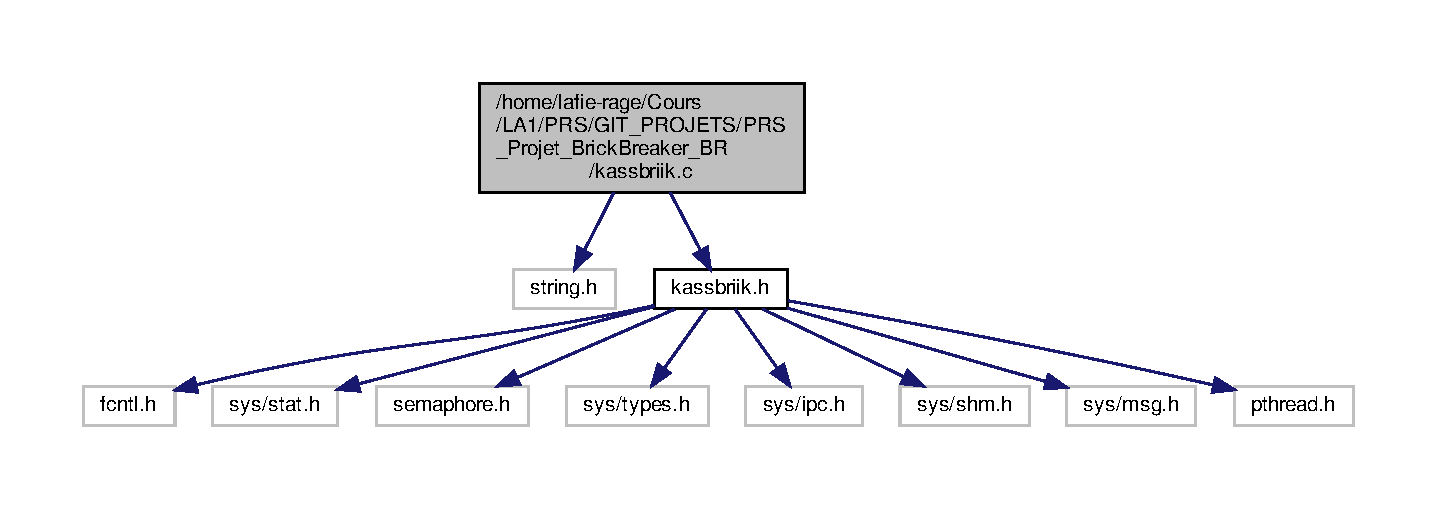
\includegraphics[width=350pt]{kassbriik_8c__incl}
\end{center}
\end{figure}
\subsection*{Functions}
\begin{DoxyCompactItemize}
\item 
void \hyperlink{kassbriik_8c_ae830f425ca982cfa3e5361fca4cbe6f0}{sort\+Score\+List} (\hyperlink{structt__scores__list}{t\+\_\+scores\+\_\+list} $\ast$scores)
\begin{DoxyCompactList}\small\item\em Sort the list if scores. \end{DoxyCompactList}\item 
void \hyperlink{kassbriik_8c_a38c0549e2a30edd606ea23cccd0ebde1}{copy\+Score\+List} (\hyperlink{structt__scores__list}{t\+\_\+scores\+\_\+list} $\ast$dest, \hyperlink{structt__scores__list}{t\+\_\+scores\+\_\+list} src)
\begin{DoxyCompactList}\small\item\em Copy a source list in the dest list. \end{DoxyCompactList}\end{DoxyCompactItemize}


\subsection{Detailed Description}
code for the game itself. 

\begin{DoxyAuthor}{Author}
Auteur Corentin Destrez, Valentin Guiberteau 
\end{DoxyAuthor}
\begin{DoxyVersion}{Version}
0.\+4 
\end{DoxyVersion}
\begin{DoxyDate}{Date}
16 april 2021
\end{DoxyDate}
This file groups all the functions applying to the game itself such as the input drawing functions. 

\subsection{Function Documentation}
\mbox{\Hypertarget{kassbriik_8c_a38c0549e2a30edd606ea23cccd0ebde1}\label{kassbriik_8c_a38c0549e2a30edd606ea23cccd0ebde1}} 
\index{kassbriik.\+c@{kassbriik.\+c}!copy\+Score\+List@{copy\+Score\+List}}
\index{copy\+Score\+List@{copy\+Score\+List}!kassbriik.\+c@{kassbriik.\+c}}
\subsubsection{\texorpdfstring{copy\+Score\+List()}{copyScoreList()}}
{\footnotesize\ttfamily void copy\+Score\+List (\begin{DoxyParamCaption}\item[{\hyperlink{structt__scores__list}{t\+\_\+scores\+\_\+list} $\ast$}]{dest,  }\item[{\hyperlink{structt__scores__list}{t\+\_\+scores\+\_\+list}}]{dest }\end{DoxyParamCaption})}



Copy a source list in the dest list. 

Copy the src list in the dest list preventing from accessing to the dest list when modifying the src list.


\begin{DoxyParams}{Parameters}
{\em dest} & The destiantion list. \\
\hline
{\em src} & The source list. \\
\hline
\end{DoxyParams}


Definition at line 36 of file kassbriik.\+c.

\mbox{\Hypertarget{kassbriik_8c_ae830f425ca982cfa3e5361fca4cbe6f0}\label{kassbriik_8c_ae830f425ca982cfa3e5361fca4cbe6f0}} 
\index{kassbriik.\+c@{kassbriik.\+c}!sort\+Score\+List@{sort\+Score\+List}}
\index{sort\+Score\+List@{sort\+Score\+List}!kassbriik.\+c@{kassbriik.\+c}}
\subsubsection{\texorpdfstring{sort\+Score\+List()}{sortScoreList()}}
{\footnotesize\ttfamily void sort\+Score\+List (\begin{DoxyParamCaption}\item[{\hyperlink{structt__scores__list}{t\+\_\+scores\+\_\+list} $\ast$}]{scores }\end{DoxyParamCaption})}



Sort the list if scores. 

/file \hyperlink{kassbriik_8c}{kassbriik.\+c} /author Corentin D\+E\+S\+T\+R\+EZ \& Valentin G\+U\+I\+B\+E\+R\+T\+E\+AU /date 12 Apr 2021 /brief Source code of the client\textquotesingle{}s library

This library containts the definition of some useful values, functions and structures that are used by the server.

Sort the score list from lower score to the greater.


\begin{DoxyParams}{Parameters}
{\em scores} & The list of scores that must be sorted. \\
\hline
\end{DoxyParams}


Definition at line 19 of file kassbriik.\+c.


\hypertarget{kassbriik_8h}{}\section{/home/lafie-\/rage/\+Cours/\+L\+A1/\+P\+R\+S/\+G\+I\+T\+\_\+\+P\+R\+O\+J\+E\+T\+S/\+P\+R\+S\+\_\+\+Projet\+\_\+\+Brick\+Breaker\+\_\+\+B\+R/kassbriik.h File Reference}
\label{kassbriik_8h}\index{/home/lafie-\/rage/\+Cours/\+L\+A1/\+P\+R\+S/\+G\+I\+T\+\_\+\+P\+R\+O\+J\+E\+T\+S/\+P\+R\+S\+\_\+\+Projet\+\_\+\+Brick\+Breaker\+\_\+\+B\+R/kassbriik.\+h@{/home/lafie-\/rage/\+Cours/\+L\+A1/\+P\+R\+S/\+G\+I\+T\+\_\+\+P\+R\+O\+J\+E\+T\+S/\+P\+R\+S\+\_\+\+Projet\+\_\+\+Brick\+Breaker\+\_\+\+B\+R/kassbriik.\+h}}
{\ttfamily \#include $<$fcntl.\+h$>$}\newline
{\ttfamily \#include $<$sys/stat.\+h$>$}\newline
{\ttfamily \#include $<$semaphore.\+h$>$}\newline
{\ttfamily \#include $<$sys/types.\+h$>$}\newline
{\ttfamily \#include $<$sys/ipc.\+h$>$}\newline
{\ttfamily \#include $<$sys/shm.\+h$>$}\newline
{\ttfamily \#include $<$sys/msg.\+h$>$}\newline
{\ttfamily \#include $<$pthread.\+h$>$}\newline
Include dependency graph for kassbriik.\+h\+:\nopagebreak
\begin{figure}[H]
\begin{center}
\leavevmode
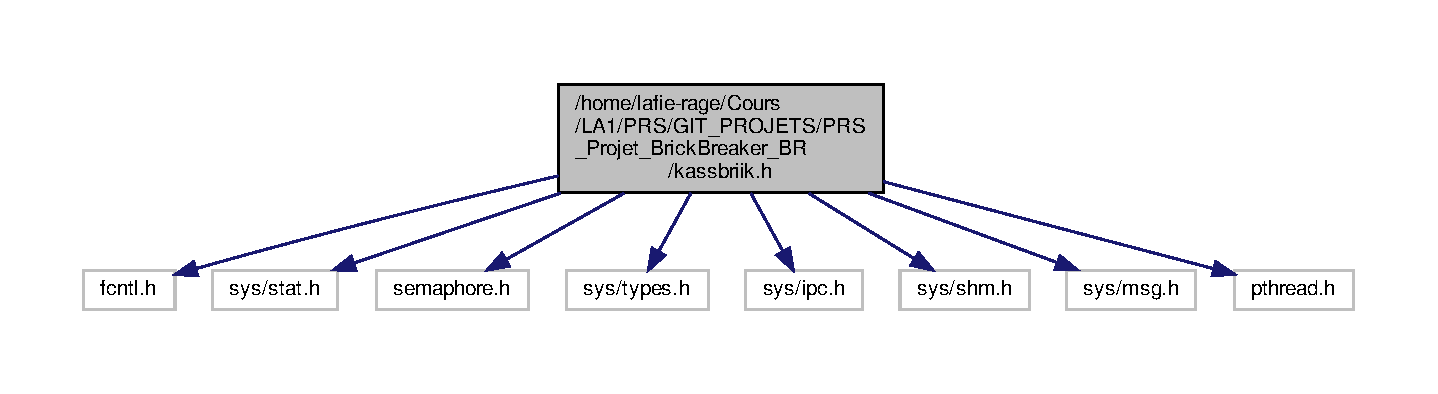
\includegraphics[width=350pt]{kassbriik_8h__incl}
\end{center}
\end{figure}
This graph shows which files directly or indirectly include this file\+:\nopagebreak
\begin{figure}[H]
\begin{center}
\leavevmode
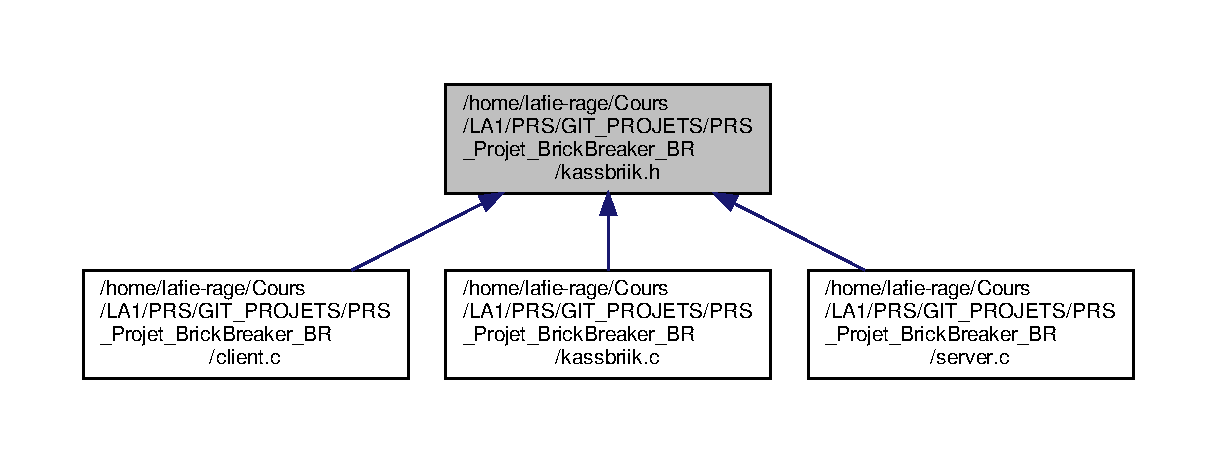
\includegraphics[width=350pt]{kassbriik_8h__dep__incl}
\end{center}
\end{figure}
\subsection*{Data Structures}
\begin{DoxyCompactItemize}
\item 
struct \hyperlink{structscore}{score}
\item 
struct \hyperlink{structscores__list}{scores\+\_\+list}
\item 
struct \hyperlink{structbody}{body}
\item 
struct \hyperlink{structrequest}{request}
\end{DoxyCompactItemize}
\subsection*{Macros}
\begin{DoxyCompactItemize}
\item 
\#define \hyperlink{kassbriik_8h_ad3fe337408f16c132c895f2b59326410}{C\+H\+E\+CK}(sts,  msg)~if ((sts) == -\/1) \{ perror(msg); exit(-\/1);\}
\begin{DoxyCompactList}\small\item\em Check the return status of a function. \end{DoxyCompactList}\item 
\#define \hyperlink{kassbriik_8h_a0a8f91f93d75a07f0ae45077db45b3eb}{M\+A\+X\+\_\+\+C\+L\+I\+E\+N\+TS}~9
\begin{DoxyCompactList}\small\item\em Number max of clients that the server can accept. \end{DoxyCompactList}\item 
\#define \hyperlink{kassbriik_8h_a53ad8675df847e45a63bcb40ff793745}{S\+E\+M\+\_\+\+S\+H\+M\+\_\+\+N\+A\+ME}~\char`\"{}kassbriik\+\_\+shm\+\_\+sem\char`\"{}
\item 
\#define \hyperlink{kassbriik_8h_a31d581c814a72a1c69bd228b078d6b69}{S\+H\+M\+\_\+\+K\+EY}~ftok(\char`\"{}/home/player/shm\+\_\+kassbriik\char`\"{}, 1)
\begin{DoxyCompactList}\small\item\em Key to acces to the shm. \end{DoxyCompactList}\item 
\#define \hyperlink{kassbriik_8h_a1a92f29d280d7de1b5bc07f16dc933bf}{M\+A\+X\+\_\+\+B\+O\+D\+Y\+\_\+\+M\+S\+G\+\_\+\+S\+I\+ZE}~256
\begin{DoxyCompactList}\small\item\em Size maximal of a message to send or read from the message queue. \end{DoxyCompactList}\item 
\#define \hyperlink{kassbriik_8h_a9fd0f43f293031d18a7b06276db6d664}{M\+S\+G\+\_\+\+M\+O\+DE}~0666
\begin{DoxyCompactList}\small\item\em Opening mode of the message queue. \end{DoxyCompactList}\item 
\#define \hyperlink{kassbriik_8h_acebb45f6d9740063956da4fc574b2b04}{M\+S\+G\+\_\+\+K\+EY}~ftok(\char`\"{}/home/player/msg\+\_\+kassbriik\char`\"{}, 1)
\begin{DoxyCompactList}\small\item\em Key ot acces to the message queue. \end{DoxyCompactList}\item 
\#define \hyperlink{kassbriik_8h_a0118c63c161e4da398fa9d4e0f11879c}{C\+O\+N\+N\+E\+C\+T\+I\+O\+N\+\_\+\+M\+S\+G\+\_\+\+T\+Y\+PE}~1
\begin{DoxyCompactList}\small\item\em Message type for client connection. \end{DoxyCompactList}\item 
\#define \hyperlink{kassbriik_8h_a0e71ded84aa1312e91ea06eed7e5c654}{C\+O\+N\+N\+E\+C\+T\+I\+O\+N\+\_\+\+N\+O\+T\+I\+F\+Y\+\_\+\+M\+SG}~\char`\"{}You are connected\char`\"{}
\begin{DoxyCompactList}\small\item\em Response of the server when the client is connected. \end{DoxyCompactList}\item 
\#define \hyperlink{kassbriik_8h_a5aace718615ca24772083216b8322d95}{S\+T\+A\+R\+T\+\_\+\+G\+A\+M\+E\+\_\+\+M\+SG}~\char`\"{}Game must start\char`\"{}
\begin{DoxyCompactList}\small\item\em Message to start the game. \end{DoxyCompactList}\item 
\#define \hyperlink{kassbriik_8h_aaeece299664ddd15098e689c50d6a5a7}{G\+A\+M\+E\+\_\+\+S\+T\+A\+R\+T\+E\+D\+\_\+\+M\+S\+G\+\_\+\+T\+Y\+PE}~2
\begin{DoxyCompactList}\small\item\em Message type to notify that the game is started. \end{DoxyCompactList}\item 
\#define \hyperlink{kassbriik_8h_a4143446cc4b5108a3ab124ac3c5b2e2e}{E\+N\+D\+\_\+\+G\+A\+M\+E\+\_\+\+M\+S\+G\+\_\+\+T\+Y\+PE}~3
\begin{DoxyCompactList}\small\item\em Message type to notify end of the game. \end{DoxyCompactList}\item 
\#define \hyperlink{kassbriik_8h_a66695a5fa7a9e8bd3257dbdafe0b256e}{S\+C\+O\+R\+E\+\_\+\+R\+E\+C\+E\+I\+V\+E\+D\+\_\+\+M\+S\+G\+\_\+\+T\+Y\+PE}~4
\begin{DoxyCompactList}\small\item\em Message type to notify that score is received. \end{DoxyCompactList}\item 
\#define \hyperlink{kassbriik_8h_ab20bc32ef9a15349cc85db5174d18364}{S\+C\+O\+R\+E\+\_\+\+W\+R\+I\+T\+T\+E\+N\+\_\+\+M\+SG}~\char`\"{}Scores can be read\char`\"{}
\begin{DoxyCompactList}\small\item\em Message send to notify that scores can be read. \end{DoxyCompactList}\item 
\#define \hyperlink{kassbriik_8h_a76c877269a8e697e34ca79d0a26665f5}{S\+C\+O\+R\+E\+\_\+\+R\+E\+A\+D\+\_\+\+M\+S\+G\+\_\+\+T\+Y\+PE}~5
\begin{DoxyCompactList}\small\item\em Message type to notify that scores has been read. \end{DoxyCompactList}\end{DoxyCompactItemize}
\subsection*{Typedefs}
\begin{DoxyCompactItemize}
\item 
typedef struct \hyperlink{structscore}{score} \hyperlink{kassbriik_8h_aceeef36f61cc8b9309737f48b70323db}{t\+\_\+score}
\item 
typedef struct \hyperlink{structscores__list}{scores\+\_\+list} \hyperlink{kassbriik_8h_a3922a6d636a23086466165dc8227070c}{t\+\_\+scores\+\_\+list}
\item 
typedef struct \hyperlink{structbody}{body} \hyperlink{kassbriik_8h_a8256930a164ca52f5a7532acc9a2725d}{t\+\_\+body}
\item 
typedef struct \hyperlink{structrequest}{request} \hyperlink{kassbriik_8h_a033810dbd32f066a84c8af1fa6b1cae7}{t\+\_\+request}
\end{DoxyCompactItemize}
\subsection*{Functions}
\begin{DoxyCompactItemize}
\item 
void \hyperlink{kassbriik_8h_ae830f425ca982cfa3e5361fca4cbe6f0}{sort\+Score\+List} (\hyperlink{structt__scores__list}{t\+\_\+scores\+\_\+list} $\ast$scores)
\begin{DoxyCompactList}\small\item\em Sort the list if scores. \end{DoxyCompactList}\item 
void \hyperlink{kassbriik_8h_a38c0549e2a30edd606ea23cccd0ebde1}{copy\+Score\+List} (\hyperlink{structt__scores__list}{t\+\_\+scores\+\_\+list} $\ast$dest, \hyperlink{structt__scores__list}{t\+\_\+scores\+\_\+list} src)
\begin{DoxyCompactList}\small\item\em Copy a source list in the dest list. \end{DoxyCompactList}\end{DoxyCompactItemize}


\subsection{Macro Definition Documentation}
\mbox{\Hypertarget{kassbriik_8h_ad3fe337408f16c132c895f2b59326410}\label{kassbriik_8h_ad3fe337408f16c132c895f2b59326410}} 
\index{kassbriik.\+h@{kassbriik.\+h}!C\+H\+E\+CK@{C\+H\+E\+CK}}
\index{C\+H\+E\+CK@{C\+H\+E\+CK}!kassbriik.\+h@{kassbriik.\+h}}
\subsubsection{\texorpdfstring{C\+H\+E\+CK}{CHECK}}
{\footnotesize\ttfamily \#define C\+H\+E\+CK(\begin{DoxyParamCaption}\item[{}]{sts,  }\item[{}]{msg }\end{DoxyParamCaption})~if ((sts) == -\/1) \{ perror(msg); exit(-\/1);\}}



Check the return status of a function. 

If the return is -\/1, priting \char`\"{}msg\char`\"{} in stderr and the errno. Then exit with -\/1 code. 

Definition at line 47 of file kassbriik.\+h.

\mbox{\Hypertarget{kassbriik_8h_a0118c63c161e4da398fa9d4e0f11879c}\label{kassbriik_8h_a0118c63c161e4da398fa9d4e0f11879c}} 
\index{kassbriik.\+h@{kassbriik.\+h}!C\+O\+N\+N\+E\+C\+T\+I\+O\+N\+\_\+\+M\+S\+G\+\_\+\+T\+Y\+PE@{C\+O\+N\+N\+E\+C\+T\+I\+O\+N\+\_\+\+M\+S\+G\+\_\+\+T\+Y\+PE}}
\index{C\+O\+N\+N\+E\+C\+T\+I\+O\+N\+\_\+\+M\+S\+G\+\_\+\+T\+Y\+PE@{C\+O\+N\+N\+E\+C\+T\+I\+O\+N\+\_\+\+M\+S\+G\+\_\+\+T\+Y\+PE}!kassbriik.\+h@{kassbriik.\+h}}
\subsubsection{\texorpdfstring{C\+O\+N\+N\+E\+C\+T\+I\+O\+N\+\_\+\+M\+S\+G\+\_\+\+T\+Y\+PE}{CONNECTION\_MSG\_TYPE}}
{\footnotesize\ttfamily \#define C\+O\+N\+N\+E\+C\+T\+I\+O\+N\+\_\+\+M\+S\+G\+\_\+\+T\+Y\+PE~1}



Message type for client connection. 

Message send by the client to connect to the server. 

Definition at line 168 of file kassbriik.\+h.

\mbox{\Hypertarget{kassbriik_8h_a0e71ded84aa1312e91ea06eed7e5c654}\label{kassbriik_8h_a0e71ded84aa1312e91ea06eed7e5c654}} 
\index{kassbriik.\+h@{kassbriik.\+h}!C\+O\+N\+N\+E\+C\+T\+I\+O\+N\+\_\+\+N\+O\+T\+I\+F\+Y\+\_\+\+M\+SG@{C\+O\+N\+N\+E\+C\+T\+I\+O\+N\+\_\+\+N\+O\+T\+I\+F\+Y\+\_\+\+M\+SG}}
\index{C\+O\+N\+N\+E\+C\+T\+I\+O\+N\+\_\+\+N\+O\+T\+I\+F\+Y\+\_\+\+M\+SG@{C\+O\+N\+N\+E\+C\+T\+I\+O\+N\+\_\+\+N\+O\+T\+I\+F\+Y\+\_\+\+M\+SG}!kassbriik.\+h@{kassbriik.\+h}}
\subsubsection{\texorpdfstring{C\+O\+N\+N\+E\+C\+T\+I\+O\+N\+\_\+\+N\+O\+T\+I\+F\+Y\+\_\+\+M\+SG}{CONNECTION\_NOTIFY\_MSG}}
{\footnotesize\ttfamily \#define C\+O\+N\+N\+E\+C\+T\+I\+O\+N\+\_\+\+N\+O\+T\+I\+F\+Y\+\_\+\+M\+SG~\char`\"{}You are connected\char`\"{}}



Response of the server when the client is connected. 



Definition at line 175 of file kassbriik.\+h.

\mbox{\Hypertarget{kassbriik_8h_a4143446cc4b5108a3ab124ac3c5b2e2e}\label{kassbriik_8h_a4143446cc4b5108a3ab124ac3c5b2e2e}} 
\index{kassbriik.\+h@{kassbriik.\+h}!E\+N\+D\+\_\+\+G\+A\+M\+E\+\_\+\+M\+S\+G\+\_\+\+T\+Y\+PE@{E\+N\+D\+\_\+\+G\+A\+M\+E\+\_\+\+M\+S\+G\+\_\+\+T\+Y\+PE}}
\index{E\+N\+D\+\_\+\+G\+A\+M\+E\+\_\+\+M\+S\+G\+\_\+\+T\+Y\+PE@{E\+N\+D\+\_\+\+G\+A\+M\+E\+\_\+\+M\+S\+G\+\_\+\+T\+Y\+PE}!kassbriik.\+h@{kassbriik.\+h}}
\subsubsection{\texorpdfstring{E\+N\+D\+\_\+\+G\+A\+M\+E\+\_\+\+M\+S\+G\+\_\+\+T\+Y\+PE}{END\_GAME\_MSG\_TYPE}}
{\footnotesize\ttfamily \#define E\+N\+D\+\_\+\+G\+A\+M\+E\+\_\+\+M\+S\+G\+\_\+\+T\+Y\+PE~3}



Message type to notify end of the game. 

Type of the message send by a client to notify the server that a player has end his game. When a message of this type is send, it must contain the score of the player. 

Definition at line 203 of file kassbriik.\+h.

\mbox{\Hypertarget{kassbriik_8h_aaeece299664ddd15098e689c50d6a5a7}\label{kassbriik_8h_aaeece299664ddd15098e689c50d6a5a7}} 
\index{kassbriik.\+h@{kassbriik.\+h}!G\+A\+M\+E\+\_\+\+S\+T\+A\+R\+T\+E\+D\+\_\+\+M\+S\+G\+\_\+\+T\+Y\+PE@{G\+A\+M\+E\+\_\+\+S\+T\+A\+R\+T\+E\+D\+\_\+\+M\+S\+G\+\_\+\+T\+Y\+PE}}
\index{G\+A\+M\+E\+\_\+\+S\+T\+A\+R\+T\+E\+D\+\_\+\+M\+S\+G\+\_\+\+T\+Y\+PE@{G\+A\+M\+E\+\_\+\+S\+T\+A\+R\+T\+E\+D\+\_\+\+M\+S\+G\+\_\+\+T\+Y\+PE}!kassbriik.\+h@{kassbriik.\+h}}
\subsubsection{\texorpdfstring{G\+A\+M\+E\+\_\+\+S\+T\+A\+R\+T\+E\+D\+\_\+\+M\+S\+G\+\_\+\+T\+Y\+PE}{GAME\_STARTED\_MSG\_TYPE}}
{\footnotesize\ttfamily \#define G\+A\+M\+E\+\_\+\+S\+T\+A\+R\+T\+E\+D\+\_\+\+M\+S\+G\+\_\+\+T\+Y\+PE~2}



Message type to notify that the game is started. 

Type of the message send by clients to the server to notify him that it has started the game. 

Definition at line 193 of file kassbriik.\+h.

\mbox{\Hypertarget{kassbriik_8h_a1a92f29d280d7de1b5bc07f16dc933bf}\label{kassbriik_8h_a1a92f29d280d7de1b5bc07f16dc933bf}} 
\index{kassbriik.\+h@{kassbriik.\+h}!M\+A\+X\+\_\+\+B\+O\+D\+Y\+\_\+\+M\+S\+G\+\_\+\+S\+I\+ZE@{M\+A\+X\+\_\+\+B\+O\+D\+Y\+\_\+\+M\+S\+G\+\_\+\+S\+I\+ZE}}
\index{M\+A\+X\+\_\+\+B\+O\+D\+Y\+\_\+\+M\+S\+G\+\_\+\+S\+I\+ZE@{M\+A\+X\+\_\+\+B\+O\+D\+Y\+\_\+\+M\+S\+G\+\_\+\+S\+I\+ZE}!kassbriik.\+h@{kassbriik.\+h}}
\subsubsection{\texorpdfstring{M\+A\+X\+\_\+\+B\+O\+D\+Y\+\_\+\+M\+S\+G\+\_\+\+S\+I\+ZE}{MAX\_BODY\_MSG\_SIZE}}
{\footnotesize\ttfamily \#define M\+A\+X\+\_\+\+B\+O\+D\+Y\+\_\+\+M\+S\+G\+\_\+\+S\+I\+ZE~256}



Size maximal of a message to send or read from the message queue. 



Definition at line 145 of file kassbriik.\+h.

\mbox{\Hypertarget{kassbriik_8h_a0a8f91f93d75a07f0ae45077db45b3eb}\label{kassbriik_8h_a0a8f91f93d75a07f0ae45077db45b3eb}} 
\index{kassbriik.\+h@{kassbriik.\+h}!M\+A\+X\+\_\+\+C\+L\+I\+E\+N\+TS@{M\+A\+X\+\_\+\+C\+L\+I\+E\+N\+TS}}
\index{M\+A\+X\+\_\+\+C\+L\+I\+E\+N\+TS@{M\+A\+X\+\_\+\+C\+L\+I\+E\+N\+TS}!kassbriik.\+h@{kassbriik.\+h}}
\subsubsection{\texorpdfstring{M\+A\+X\+\_\+\+C\+L\+I\+E\+N\+TS}{MAX\_CLIENTS}}
{\footnotesize\ttfamily \#define M\+A\+X\+\_\+\+C\+L\+I\+E\+N\+TS~9}



Number max of clients that the server can accept. 



Definition at line 54 of file kassbriik.\+h.

\mbox{\Hypertarget{kassbriik_8h_acebb45f6d9740063956da4fc574b2b04}\label{kassbriik_8h_acebb45f6d9740063956da4fc574b2b04}} 
\index{kassbriik.\+h@{kassbriik.\+h}!M\+S\+G\+\_\+\+K\+EY@{M\+S\+G\+\_\+\+K\+EY}}
\index{M\+S\+G\+\_\+\+K\+EY@{M\+S\+G\+\_\+\+K\+EY}!kassbriik.\+h@{kassbriik.\+h}}
\subsubsection{\texorpdfstring{M\+S\+G\+\_\+\+K\+EY}{MSG\_KEY}}
{\footnotesize\ttfamily \#define M\+S\+G\+\_\+\+K\+EY~ftok(\char`\"{}/home/player/msg\+\_\+kassbriik\char`\"{}, 1)}



Key ot acces to the message queue. 



Definition at line 159 of file kassbriik.\+h.

\mbox{\Hypertarget{kassbriik_8h_a9fd0f43f293031d18a7b06276db6d664}\label{kassbriik_8h_a9fd0f43f293031d18a7b06276db6d664}} 
\index{kassbriik.\+h@{kassbriik.\+h}!M\+S\+G\+\_\+\+M\+O\+DE@{M\+S\+G\+\_\+\+M\+O\+DE}}
\index{M\+S\+G\+\_\+\+M\+O\+DE@{M\+S\+G\+\_\+\+M\+O\+DE}!kassbriik.\+h@{kassbriik.\+h}}
\subsubsection{\texorpdfstring{M\+S\+G\+\_\+\+M\+O\+DE}{MSG\_MODE}}
{\footnotesize\ttfamily \#define M\+S\+G\+\_\+\+M\+O\+DE~0666}



Opening mode of the message queue. 



Definition at line 152 of file kassbriik.\+h.

\mbox{\Hypertarget{kassbriik_8h_a76c877269a8e697e34ca79d0a26665f5}\label{kassbriik_8h_a76c877269a8e697e34ca79d0a26665f5}} 
\index{kassbriik.\+h@{kassbriik.\+h}!S\+C\+O\+R\+E\+\_\+\+R\+E\+A\+D\+\_\+\+M\+S\+G\+\_\+\+T\+Y\+PE@{S\+C\+O\+R\+E\+\_\+\+R\+E\+A\+D\+\_\+\+M\+S\+G\+\_\+\+T\+Y\+PE}}
\index{S\+C\+O\+R\+E\+\_\+\+R\+E\+A\+D\+\_\+\+M\+S\+G\+\_\+\+T\+Y\+PE@{S\+C\+O\+R\+E\+\_\+\+R\+E\+A\+D\+\_\+\+M\+S\+G\+\_\+\+T\+Y\+PE}!kassbriik.\+h@{kassbriik.\+h}}
\subsubsection{\texorpdfstring{S\+C\+O\+R\+E\+\_\+\+R\+E\+A\+D\+\_\+\+M\+S\+G\+\_\+\+T\+Y\+PE}{SCORE\_READ\_MSG\_TYPE}}
{\footnotesize\ttfamily \#define S\+C\+O\+R\+E\+\_\+\+R\+E\+A\+D\+\_\+\+M\+S\+G\+\_\+\+T\+Y\+PE~5}



Message type to notify that scores has been read. 

Type of the message send by the server to notify a client that it has read the scores. 

Definition at line 230 of file kassbriik.\+h.

\mbox{\Hypertarget{kassbriik_8h_a66695a5fa7a9e8bd3257dbdafe0b256e}\label{kassbriik_8h_a66695a5fa7a9e8bd3257dbdafe0b256e}} 
\index{kassbriik.\+h@{kassbriik.\+h}!S\+C\+O\+R\+E\+\_\+\+R\+E\+C\+E\+I\+V\+E\+D\+\_\+\+M\+S\+G\+\_\+\+T\+Y\+PE@{S\+C\+O\+R\+E\+\_\+\+R\+E\+C\+E\+I\+V\+E\+D\+\_\+\+M\+S\+G\+\_\+\+T\+Y\+PE}}
\index{S\+C\+O\+R\+E\+\_\+\+R\+E\+C\+E\+I\+V\+E\+D\+\_\+\+M\+S\+G\+\_\+\+T\+Y\+PE@{S\+C\+O\+R\+E\+\_\+\+R\+E\+C\+E\+I\+V\+E\+D\+\_\+\+M\+S\+G\+\_\+\+T\+Y\+PE}!kassbriik.\+h@{kassbriik.\+h}}
\subsubsection{\texorpdfstring{S\+C\+O\+R\+E\+\_\+\+R\+E\+C\+E\+I\+V\+E\+D\+\_\+\+M\+S\+G\+\_\+\+T\+Y\+PE}{SCORE\_RECEIVED\_MSG\_TYPE}}
{\footnotesize\ttfamily \#define S\+C\+O\+R\+E\+\_\+\+R\+E\+C\+E\+I\+V\+E\+D\+\_\+\+M\+S\+G\+\_\+\+T\+Y\+PE~4}



Message type to notify that score is received. 

Type of the message send by the server to notify a client that it has received its player\textquotesingle{}s score. 

Definition at line 212 of file kassbriik.\+h.

\mbox{\Hypertarget{kassbriik_8h_ab20bc32ef9a15349cc85db5174d18364}\label{kassbriik_8h_ab20bc32ef9a15349cc85db5174d18364}} 
\index{kassbriik.\+h@{kassbriik.\+h}!S\+C\+O\+R\+E\+\_\+\+W\+R\+I\+T\+T\+E\+N\+\_\+\+M\+SG@{S\+C\+O\+R\+E\+\_\+\+W\+R\+I\+T\+T\+E\+N\+\_\+\+M\+SG}}
\index{S\+C\+O\+R\+E\+\_\+\+W\+R\+I\+T\+T\+E\+N\+\_\+\+M\+SG@{S\+C\+O\+R\+E\+\_\+\+W\+R\+I\+T\+T\+E\+N\+\_\+\+M\+SG}!kassbriik.\+h@{kassbriik.\+h}}
\subsubsection{\texorpdfstring{S\+C\+O\+R\+E\+\_\+\+W\+R\+I\+T\+T\+E\+N\+\_\+\+M\+SG}{SCORE\_WRITTEN\_MSG}}
{\footnotesize\ttfamily \#define S\+C\+O\+R\+E\+\_\+\+W\+R\+I\+T\+T\+E\+N\+\_\+\+M\+SG~\char`\"{}Scores can be read\char`\"{}}



Message send to notify that scores can be read. 

Message send to a client to notify him that he can read the scores in the shm 

Definition at line 221 of file kassbriik.\+h.

\mbox{\Hypertarget{kassbriik_8h_a53ad8675df847e45a63bcb40ff793745}\label{kassbriik_8h_a53ad8675df847e45a63bcb40ff793745}} 
\index{kassbriik.\+h@{kassbriik.\+h}!S\+E\+M\+\_\+\+S\+H\+M\+\_\+\+N\+A\+ME@{S\+E\+M\+\_\+\+S\+H\+M\+\_\+\+N\+A\+ME}}
\index{S\+E\+M\+\_\+\+S\+H\+M\+\_\+\+N\+A\+ME@{S\+E\+M\+\_\+\+S\+H\+M\+\_\+\+N\+A\+ME}!kassbriik.\+h@{kassbriik.\+h}}
\subsubsection{\texorpdfstring{S\+E\+M\+\_\+\+S\+H\+M\+\_\+\+N\+A\+ME}{SEM\_SHM\_NAME}}
{\footnotesize\ttfamily \#define S\+E\+M\+\_\+\+S\+H\+M\+\_\+\+N\+A\+ME~\char`\"{}kassbriik\+\_\+shm\+\_\+sem\char`\"{}}



Definition at line 69 of file kassbriik.\+h.

\mbox{\Hypertarget{kassbriik_8h_a31d581c814a72a1c69bd228b078d6b69}\label{kassbriik_8h_a31d581c814a72a1c69bd228b078d6b69}} 
\index{kassbriik.\+h@{kassbriik.\+h}!S\+H\+M\+\_\+\+K\+EY@{S\+H\+M\+\_\+\+K\+EY}}
\index{S\+H\+M\+\_\+\+K\+EY@{S\+H\+M\+\_\+\+K\+EY}!kassbriik.\+h@{kassbriik.\+h}}
\subsubsection{\texorpdfstring{S\+H\+M\+\_\+\+K\+EY}{SHM\_KEY}}
{\footnotesize\ttfamily \#define S\+H\+M\+\_\+\+K\+EY~ftok(\char`\"{}/home/player/shm\+\_\+kassbriik\char`\"{}, 1)}



Key to acces to the shm. 



Definition at line 84 of file kassbriik.\+h.

\mbox{\Hypertarget{kassbriik_8h_a5aace718615ca24772083216b8322d95}\label{kassbriik_8h_a5aace718615ca24772083216b8322d95}} 
\index{kassbriik.\+h@{kassbriik.\+h}!S\+T\+A\+R\+T\+\_\+\+G\+A\+M\+E\+\_\+\+M\+SG@{S\+T\+A\+R\+T\+\_\+\+G\+A\+M\+E\+\_\+\+M\+SG}}
\index{S\+T\+A\+R\+T\+\_\+\+G\+A\+M\+E\+\_\+\+M\+SG@{S\+T\+A\+R\+T\+\_\+\+G\+A\+M\+E\+\_\+\+M\+SG}!kassbriik.\+h@{kassbriik.\+h}}
\subsubsection{\texorpdfstring{S\+T\+A\+R\+T\+\_\+\+G\+A\+M\+E\+\_\+\+M\+SG}{START\_GAME\_MSG}}
{\footnotesize\ttfamily \#define S\+T\+A\+R\+T\+\_\+\+G\+A\+M\+E\+\_\+\+M\+SG~\char`\"{}Game must start\char`\"{}}



Message to start the game. 

The message send by server to all clients to notify them that they must start the game. 

Definition at line 184 of file kassbriik.\+h.



\subsection{Typedef Documentation}
\mbox{\Hypertarget{kassbriik_8h_a8256930a164ca52f5a7532acc9a2725d}\label{kassbriik_8h_a8256930a164ca52f5a7532acc9a2725d}} 
\index{kassbriik.\+h@{kassbriik.\+h}!t\+\_\+body@{t\+\_\+body}}
\index{t\+\_\+body@{t\+\_\+body}!kassbriik.\+h@{kassbriik.\+h}}
\subsubsection{\texorpdfstring{t\+\_\+body}{t\_body}}
{\footnotesize\ttfamily typedef struct \hyperlink{structbody}{body}  \hyperlink{structt__body}{t\+\_\+body}}

\mbox{\Hypertarget{kassbriik_8h_a033810dbd32f066a84c8af1fa6b1cae7}\label{kassbriik_8h_a033810dbd32f066a84c8af1fa6b1cae7}} 
\index{kassbriik.\+h@{kassbriik.\+h}!t\+\_\+request@{t\+\_\+request}}
\index{t\+\_\+request@{t\+\_\+request}!kassbriik.\+h@{kassbriik.\+h}}
\subsubsection{\texorpdfstring{t\+\_\+request}{t\_request}}
{\footnotesize\ttfamily typedef struct \hyperlink{structrequest}{request}  \hyperlink{structt__request}{t\+\_\+request}}

\mbox{\Hypertarget{kassbriik_8h_aceeef36f61cc8b9309737f48b70323db}\label{kassbriik_8h_aceeef36f61cc8b9309737f48b70323db}} 
\index{kassbriik.\+h@{kassbriik.\+h}!t\+\_\+score@{t\+\_\+score}}
\index{t\+\_\+score@{t\+\_\+score}!kassbriik.\+h@{kassbriik.\+h}}
\subsubsection{\texorpdfstring{t\+\_\+score}{t\_score}}
{\footnotesize\ttfamily typedef struct \hyperlink{structscore}{score}  \hyperlink{structt__score}{t\+\_\+score}}

\mbox{\Hypertarget{kassbriik_8h_a3922a6d636a23086466165dc8227070c}\label{kassbriik_8h_a3922a6d636a23086466165dc8227070c}} 
\index{kassbriik.\+h@{kassbriik.\+h}!t\+\_\+scores\+\_\+list@{t\+\_\+scores\+\_\+list}}
\index{t\+\_\+scores\+\_\+list@{t\+\_\+scores\+\_\+list}!kassbriik.\+h@{kassbriik.\+h}}
\subsubsection{\texorpdfstring{t\+\_\+scores\+\_\+list}{t\_scores\_list}}
{\footnotesize\ttfamily typedef struct \hyperlink{structscores__list}{scores\+\_\+list}  \hyperlink{structt__scores__list}{t\+\_\+scores\+\_\+list}}



\subsection{Function Documentation}
\mbox{\Hypertarget{kassbriik_8h_a38c0549e2a30edd606ea23cccd0ebde1}\label{kassbriik_8h_a38c0549e2a30edd606ea23cccd0ebde1}} 
\index{kassbriik.\+h@{kassbriik.\+h}!copy\+Score\+List@{copy\+Score\+List}}
\index{copy\+Score\+List@{copy\+Score\+List}!kassbriik.\+h@{kassbriik.\+h}}
\subsubsection{\texorpdfstring{copy\+Score\+List()}{copyScoreList()}}
{\footnotesize\ttfamily void copy\+Score\+List (\begin{DoxyParamCaption}\item[{\hyperlink{structt__scores__list}{t\+\_\+scores\+\_\+list} $\ast$}]{dest,  }\item[{\hyperlink{structt__scores__list}{t\+\_\+scores\+\_\+list}}]{src }\end{DoxyParamCaption})}



Copy a source list in the dest list. 

Copy the src list in the dest list preventing from accessing to the dest list when modifying the src list.


\begin{DoxyParams}{Parameters}
{\em dest} & The destiantion list. \\
\hline
{\em src} & The source list. \\
\hline
\end{DoxyParams}


Definition at line 36 of file kassbriik.\+c.

\mbox{\Hypertarget{kassbriik_8h_ae830f425ca982cfa3e5361fca4cbe6f0}\label{kassbriik_8h_ae830f425ca982cfa3e5361fca4cbe6f0}} 
\index{kassbriik.\+h@{kassbriik.\+h}!sort\+Score\+List@{sort\+Score\+List}}
\index{sort\+Score\+List@{sort\+Score\+List}!kassbriik.\+h@{kassbriik.\+h}}
\subsubsection{\texorpdfstring{sort\+Score\+List()}{sortScoreList()}}
{\footnotesize\ttfamily void sort\+Score\+List (\begin{DoxyParamCaption}\item[{\hyperlink{structt__scores__list}{t\+\_\+scores\+\_\+list} $\ast$}]{scores }\end{DoxyParamCaption})}



Sort the list if scores. 

/file \hyperlink{kassbriik_8c}{kassbriik.\+c} /author Corentin D\+E\+S\+T\+R\+EZ \& Valentin G\+U\+I\+B\+E\+R\+T\+E\+AU /date 12 Apr 2021 /brief Source code of the client\textquotesingle{}s library

This library containts the definition of some useful values, functions and structures that are used by the server.

Sort the score list from lower score to the greater.


\begin{DoxyParams}{Parameters}
{\em scores} & The list of scores that must be sorted. \\
\hline
\end{DoxyParams}


Definition at line 19 of file kassbriik.\+c.


\hypertarget{_r_e_a_d_m_e_8en_8md}{}\section{/home/lafie-\/rage/\+Cours/\+L\+A1/\+P\+R\+S/\+G\+I\+T\+\_\+\+P\+R\+O\+J\+E\+T\+S/\+P\+R\+S\+\_\+\+Projet\+\_\+\+Brick\+Breaker\+\_\+\+B\+R/\+R\+E\+A\+D\+ME.en.\+md File Reference}
\label{_r_e_a_d_m_e_8en_8md}\index{/home/lafie-\/rage/\+Cours/\+L\+A1/\+P\+R\+S/\+G\+I\+T\+\_\+\+P\+R\+O\+J\+E\+T\+S/\+P\+R\+S\+\_\+\+Projet\+\_\+\+Brick\+Breaker\+\_\+\+B\+R/\+R\+E\+A\+D\+M\+E.\+en.\+md@{/home/lafie-\/rage/\+Cours/\+L\+A1/\+P\+R\+S/\+G\+I\+T\+\_\+\+P\+R\+O\+J\+E\+T\+S/\+P\+R\+S\+\_\+\+Projet\+\_\+\+Brick\+Breaker\+\_\+\+B\+R/\+R\+E\+A\+D\+M\+E.\+en.\+md}}

\hypertarget{_r_e_a_d_m_e_8fr_8md}{}\section{/home/lafie-\/rage/\+Cours/\+L\+A1/\+P\+R\+S/\+G\+I\+T\+\_\+\+P\+R\+O\+J\+E\+T\+S/\+P\+R\+S\+\_\+\+Projet\+\_\+\+Brick\+Breaker\+\_\+\+B\+R/\+R\+E\+A\+D\+ME.fr.\+md File Reference}
\label{_r_e_a_d_m_e_8fr_8md}\index{/home/lafie-\/rage/\+Cours/\+L\+A1/\+P\+R\+S/\+G\+I\+T\+\_\+\+P\+R\+O\+J\+E\+T\+S/\+P\+R\+S\+\_\+\+Projet\+\_\+\+Brick\+Breaker\+\_\+\+B\+R/\+R\+E\+A\+D\+M\+E.\+fr.\+md@{/home/lafie-\/rage/\+Cours/\+L\+A1/\+P\+R\+S/\+G\+I\+T\+\_\+\+P\+R\+O\+J\+E\+T\+S/\+P\+R\+S\+\_\+\+Projet\+\_\+\+Brick\+Breaker\+\_\+\+B\+R/\+R\+E\+A\+D\+M\+E.\+fr.\+md}}

\hypertarget{_r_e_a_d_m_e_8md}{}\section{/home/lafie-\/rage/\+Cours/\+L\+A1/\+P\+R\+S/\+G\+I\+T\+\_\+\+P\+R\+O\+J\+E\+T\+S/\+P\+R\+S\+\_\+\+Projet\+\_\+\+Brick\+Breaker\+\_\+\+B\+R/\+R\+E\+A\+D\+ME.md File Reference}
\label{_r_e_a_d_m_e_8md}\index{/home/lafie-\/rage/\+Cours/\+L\+A1/\+P\+R\+S/\+G\+I\+T\+\_\+\+P\+R\+O\+J\+E\+T\+S/\+P\+R\+S\+\_\+\+Projet\+\_\+\+Brick\+Breaker\+\_\+\+B\+R/\+R\+E\+A\+D\+M\+E.\+md@{/home/lafie-\/rage/\+Cours/\+L\+A1/\+P\+R\+S/\+G\+I\+T\+\_\+\+P\+R\+O\+J\+E\+T\+S/\+P\+R\+S\+\_\+\+Projet\+\_\+\+Brick\+Breaker\+\_\+\+B\+R/\+R\+E\+A\+D\+M\+E.\+md}}

\hypertarget{server_8c}{}\section{/home/lafie-\/rage/\+Cours/\+L\+A1/\+P\+R\+S/\+G\+I\+T\+\_\+\+P\+R\+O\+J\+E\+T\+S/\+P\+R\+S\+\_\+\+Projet\+\_\+\+Brick\+Breaker\+\_\+\+B\+R/server.c File Reference}
\label{server_8c}\index{/home/lafie-\/rage/\+Cours/\+L\+A1/\+P\+R\+S/\+G\+I\+T\+\_\+\+P\+R\+O\+J\+E\+T\+S/\+P\+R\+S\+\_\+\+Projet\+\_\+\+Brick\+Breaker\+\_\+\+B\+R/server.\+c@{/home/lafie-\/rage/\+Cours/\+L\+A1/\+P\+R\+S/\+G\+I\+T\+\_\+\+P\+R\+O\+J\+E\+T\+S/\+P\+R\+S\+\_\+\+Projet\+\_\+\+Brick\+Breaker\+\_\+\+B\+R/server.\+c}}


Source code of the client library.  


{\ttfamily \#include $<$stdio.\+h$>$}\newline
{\ttfamily \#include $<$stdlib.\+h$>$}\newline
{\ttfamily \#include $<$unistd.\+h$>$}\newline
{\ttfamily \#include $<$string.\+h$>$}\newline
{\ttfamily \#include \char`\"{}kassbriik.\+h\char`\"{}}\newline
{\ttfamily \#include \char`\"{}server\+\_\+kassbriik.\+h\char`\"{}}\newline
Include dependency graph for server.\+c\+:\nopagebreak
\begin{figure}[H]
\begin{center}
\leavevmode
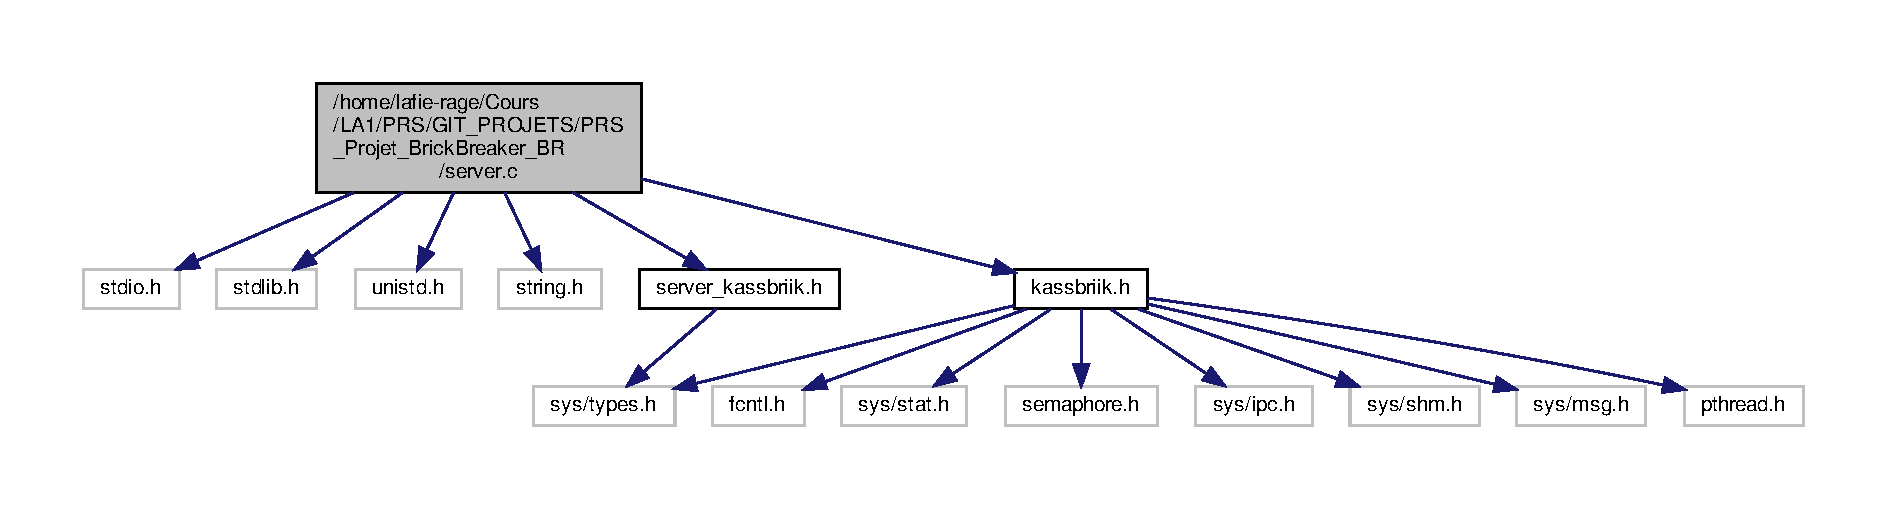
\includegraphics[width=350pt]{server_8c__incl}
\end{center}
\end{figure}
\subsection*{Functions}
\begin{DoxyCompactItemize}
\item 
void \hyperlink{server_8c_ac35a96447f088b28de93f9902ad7be97}{get\+Message\+Queue} (int $\ast$msg\+Id)
\begin{DoxyCompactList}\small\item\em Create the message queue to communicate between the serveur and the client. \end{DoxyCompactList}\item 
void \hyperlink{server_8c_a03d60fb910e6f6596cfbaf9d0d549c5e}{retrieve\+Clients\+Informations} (int msg\+Id, \hyperlink{server__kassbriik_8h_a0a2d0fa87306441ee5e7772d478fb8e4}{t\+\_\+clients\+\_\+list} $\ast$clients, int nb\+Of\+Clients\+To\+Wait)
\begin{DoxyCompactList}\small\item\em Await for clients\textquotesingle{} message to get their pid and the player\textquotesingle{}s username. \end{DoxyCompactList}\item 
void \hyperlink{server_8c_a98cd9db04337a41311bff8d710bbc2fa}{confirm\+Connection\+To\+Client} (int msg\+Id, int client\+Pid, const char $\ast$buffer)
\begin{DoxyCompactList}\small\item\em Send a message to a client via the message queue to confirm connection. \end{DoxyCompactList}\item 
void \hyperlink{server_8c_a3117517939bbf27ad242fcd543d3250c}{notify\+Clients} (int msg\+Id, \hyperlink{server__kassbriik_8h_a0a2d0fa87306441ee5e7772d478fb8e4}{t\+\_\+clients\+\_\+list} clients, const char $\ast$buffer)
\begin{DoxyCompactList}\small\item\em Send a message to multiple clients via the message queue. \end{DoxyCompactList}\item 
void \hyperlink{server_8c_a99ae9684bd61dfacc6c3cdfd6c477f20}{waiting\+Clients\+Response} (int msg\+Id, \hyperlink{server__kassbriik_8h_a0a2d0fa87306441ee5e7772d478fb8e4}{t\+\_\+clients\+\_\+list} clients, int msg\+Type)
\item 
void \hyperlink{server_8c_a2e8cb63dd11a9af1049d001fe86d7f96}{waiting\+Players\+Score} (int msg\+Id, \hyperlink{server__kassbriik_8h_a0a2d0fa87306441ee5e7772d478fb8e4}{t\+\_\+clients\+\_\+list} $\ast$clients)
\begin{DoxyCompactList}\small\item\em Await the all clients in the list to send their score. \end{DoxyCompactList}\item 
void \hyperlink{server_8c_ab28dcc1302fd208ab180785497949d2d}{create\+And\+Open\+Shm\+And\+Semaphore} (int $\ast$shm\+Id, struct shmid\+\_\+ds $\ast$shm\+Buffer, \hyperlink{structt__scores__list}{t\+\_\+scores\+\_\+list} $\ast$$\ast$shm\+Ptr, sem\+\_\+t $\ast$sem\+Id)
\begin{DoxyCompactList}\small\item\em Create and open the shm and its semaphore. \end{DoxyCompactList}\item 
void \hyperlink{server_8c_ac523a7ce31323a926b20ed893000c4a1}{write\+Players\+Score} (int msg\+Id, \hyperlink{server__kassbriik_8h_a0a2d0fa87306441ee5e7772d478fb8e4}{t\+\_\+clients\+\_\+list} clients, int $\ast$shm\+Id, struct shmid\+\_\+ds $\ast$shm\+Buffer)
\item 
int \hyperlink{server_8c_a0ddf1224851353fc92bfbff6f499fa97}{main} (int argc, char $\ast$argv\mbox{[}$\,$\mbox{]})
\end{DoxyCompactItemize}


\subsection{Detailed Description}
Source code of the client library. 

\begin{DoxyAuthor}{Author}
Corentin D\+E\+S\+T\+R\+EZ \& Valentin G\+U\+I\+B\+E\+R\+T\+E\+AU 
\end{DoxyAuthor}
\begin{DoxyVersion}{Version}
1.\+0 
\end{DoxyVersion}
\begin{DoxyDate}{Date}
09 Apr 2021 This file containts the functions defining the behavior of the server. It also define its behavior depending on the messages recieved. 
\end{DoxyDate}


\subsection{Function Documentation}
\mbox{\Hypertarget{server_8c_a98cd9db04337a41311bff8d710bbc2fa}\label{server_8c_a98cd9db04337a41311bff8d710bbc2fa}} 
\index{server.\+c@{server.\+c}!confirm\+Connection\+To\+Client@{confirm\+Connection\+To\+Client}}
\index{confirm\+Connection\+To\+Client@{confirm\+Connection\+To\+Client}!server.\+c@{server.\+c}}
\subsubsection{\texorpdfstring{confirm\+Connection\+To\+Client()}{confirmConnectionToClient()}}
{\footnotesize\ttfamily void confirm\+Connection\+To\+Client (\begin{DoxyParamCaption}\item[{int}]{msg\+Id,  }\item[{int}]{type,  }\item[{const char $\ast$}]{msg }\end{DoxyParamCaption})}



Send a message to a client via the message queue to confirm connection. 

Send the message to a client which pid is send as argument. The message is composed of the message as string to send, the pid of the destination client and the pid of the server.


\begin{DoxyParams}{Parameters}
{\em msg\+Id} & Pointer where the file descriptor of the message queue that must be used. \\
\hline
{\em client\+Pid} & The pid of the destination client. \\
\hline
{\em buffer} & The string that will be send in the message. \\
\hline
\end{DoxyParams}


Definition at line 189 of file server.\+c.

\mbox{\Hypertarget{server_8c_ab28dcc1302fd208ab180785497949d2d}\label{server_8c_ab28dcc1302fd208ab180785497949d2d}} 
\index{server.\+c@{server.\+c}!create\+And\+Open\+Shm\+And\+Semaphore@{create\+And\+Open\+Shm\+And\+Semaphore}}
\index{create\+And\+Open\+Shm\+And\+Semaphore@{create\+And\+Open\+Shm\+And\+Semaphore}!server.\+c@{server.\+c}}
\subsubsection{\texorpdfstring{create\+And\+Open\+Shm\+And\+Semaphore()}{createAndOpenShmAndSemaphore()}}
{\footnotesize\ttfamily void create\+And\+Open\+Shm\+And\+Semaphore (\begin{DoxyParamCaption}\item[{int $\ast$}]{shm\+Id,  }\item[{struct shmid\+\_\+ds $\ast$}]{shm\+Buffer,  }\item[{\hyperlink{structt__scores__list}{t\+\_\+scores\+\_\+list} $\ast$$\ast$}]{shm\+Ptr,  }\item[{sem\+\_\+t $\ast$}]{sem\+Id }\end{DoxyParamCaption})}



Create and open the shm and its semaphore. 

If the shm exists, delete it. In any case create the shm and open it. Then set the shm\+Buffer with the shm\textquotesingle{}s infos. If the semaphore already exists, close it. In any case create the semaphore and open it.


\begin{DoxyParams}{Parameters}
{\em shm\+Id} & The id of the shm. \\
\hline
{\em shm\+Buffer} & The buffer that must contains the shmid\+\_\+ds struct of the shm. \\
\hline
{\em shm\+Ptr} & The pointer to the shm used to read and write through it. \\
\hline
{\em sem\+Id} & The pointer to the semaphore. \\
\hline
\end{DoxyParams}


Definition at line 241 of file server.\+c.

\mbox{\Hypertarget{server_8c_ac35a96447f088b28de93f9902ad7be97}\label{server_8c_ac35a96447f088b28de93f9902ad7be97}} 
\index{server.\+c@{server.\+c}!get\+Message\+Queue@{get\+Message\+Queue}}
\index{get\+Message\+Queue@{get\+Message\+Queue}!server.\+c@{server.\+c}}
\subsubsection{\texorpdfstring{get\+Message\+Queue()}{getMessageQueue()}}
{\footnotesize\ttfamily void get\+Message\+Queue (\begin{DoxyParamCaption}\item[{int $\ast$}]{msg\+Id }\end{DoxyParamCaption})}



Create the message queue to communicate between the serveur and the client. 

Verify if the message queue isn\textquotesingle{}t already created. If it is, delete it. In any case, end by creating the message queue and store is id in msg\+Id.


\begin{DoxyParams}{Parameters}
{\em msg\+Id} & Pointer where the file descriptor of the message queue will be stored. \\
\hline
\end{DoxyParams}


Definition at line 183 of file server.\+c.

\mbox{\Hypertarget{server_8c_a0ddf1224851353fc92bfbff6f499fa97}\label{server_8c_a0ddf1224851353fc92bfbff6f499fa97}} 
\index{server.\+c@{server.\+c}!main@{main}}
\index{main@{main}!server.\+c@{server.\+c}}
\subsubsection{\texorpdfstring{main()}{main()}}
{\footnotesize\ttfamily int main (\begin{DoxyParamCaption}\item[{int}]{argc,  }\item[{char $\ast$}]{argv\mbox{[}$\,$\mbox{]} }\end{DoxyParamCaption})}



Definition at line 134 of file server.\+c.

\mbox{\Hypertarget{server_8c_a3117517939bbf27ad242fcd543d3250c}\label{server_8c_a3117517939bbf27ad242fcd543d3250c}} 
\index{server.\+c@{server.\+c}!notify\+Clients@{notify\+Clients}}
\index{notify\+Clients@{notify\+Clients}!server.\+c@{server.\+c}}
\subsubsection{\texorpdfstring{notify\+Clients()}{notifyClients()}}
{\footnotesize\ttfamily void notify\+Clients (\begin{DoxyParamCaption}\item[{int}]{msg\+Id,  }\item[{\hyperlink{server__kassbriik_8h_a0a2d0fa87306441ee5e7772d478fb8e4}{t\+\_\+clients\+\_\+list}}]{clients,  }\item[{const char $\ast$}]{buffer }\end{DoxyParamCaption})}



Send a message to multiple clients via the message queue. 

Send the message to a list of clients that is send as argument. The message is composed of the message as string to send and the pid of the server. Its type will be the pid of the client whose message is destinated.


\begin{DoxyParams}{Parameters}
{\em msg\+Id} & Pointer where the file descriptor of the message queue that must be used. \\
\hline
{\em clients} & The list of the clients that will be notified. \\
\hline
{\em buffer} & The string that will be send in the message. \\
\hline
\end{DoxyParams}


Definition at line 198 of file server.\+c.

\mbox{\Hypertarget{server_8c_a03d60fb910e6f6596cfbaf9d0d549c5e}\label{server_8c_a03d60fb910e6f6596cfbaf9d0d549c5e}} 
\index{server.\+c@{server.\+c}!retrieve\+Clients\+Informations@{retrieve\+Clients\+Informations}}
\index{retrieve\+Clients\+Informations@{retrieve\+Clients\+Informations}!server.\+c@{server.\+c}}
\subsubsection{\texorpdfstring{retrieve\+Clients\+Informations()}{retrieveClientsInformations()}}
{\footnotesize\ttfamily void retrieve\+Clients\+Informations (\begin{DoxyParamCaption}\item[{int}]{msg\+Id,  }\item[{\hyperlink{server__kassbriik_8h_a0a2d0fa87306441ee5e7772d478fb8e4}{t\+\_\+clients\+\_\+list} $\ast$}]{clients,  }\item[{int}]{nb\+Of\+Clients\+To\+Wait }\end{DoxyParamCaption})}



Await for clients\textquotesingle{} message to get their pid and the player\textquotesingle{}s username. 

Await for clients\textquotesingle{} message to get their pid and the player\textquotesingle{}s username and store it in the clients list send in parameters.


\begin{DoxyParams}{Parameters}
{\em msg\+Id} & Pointer where the file descriptor of the message queue that must be used. \\
\hline
{\em clients} & The list of clients where the client\textquotesingle{}s informations will be stored. \\
\hline
{\em nb\+Of\+Clients\+To\+Wait} & The number of clients that the server will get informations. \\
\hline
\end{DoxyParams}


Definition at line 168 of file server.\+c.

\mbox{\Hypertarget{server_8c_a99ae9684bd61dfacc6c3cdfd6c477f20}\label{server_8c_a99ae9684bd61dfacc6c3cdfd6c477f20}} 
\index{server.\+c@{server.\+c}!waiting\+Clients\+Response@{waiting\+Clients\+Response}}
\index{waiting\+Clients\+Response@{waiting\+Clients\+Response}!server.\+c@{server.\+c}}
\subsubsection{\texorpdfstring{waiting\+Clients\+Response()}{waitingClientsResponse()}}
{\footnotesize\ttfamily void waiting\+Clients\+Response (\begin{DoxyParamCaption}\item[{int}]{msg\+Id,  }\item[{\hyperlink{server__kassbriik_8h_a0a2d0fa87306441ee5e7772d478fb8e4}{t\+\_\+clients\+\_\+list}}]{clients,  }\item[{int}]{msg\+Type }\end{DoxyParamCaption})}



Definition at line 210 of file server.\+c.

\mbox{\Hypertarget{server_8c_a2e8cb63dd11a9af1049d001fe86d7f96}\label{server_8c_a2e8cb63dd11a9af1049d001fe86d7f96}} 
\index{server.\+c@{server.\+c}!waiting\+Players\+Score@{waiting\+Players\+Score}}
\index{waiting\+Players\+Score@{waiting\+Players\+Score}!server.\+c@{server.\+c}}
\subsubsection{\texorpdfstring{waiting\+Players\+Score()}{waitingPlayersScore()}}
{\footnotesize\ttfamily void waiting\+Players\+Score (\begin{DoxyParamCaption}\item[{int}]{msg\+Id,  }\item[{\hyperlink{server__kassbriik_8h_a0a2d0fa87306441ee5e7772d478fb8e4}{t\+\_\+clients\+\_\+list} $\ast$}]{clients }\end{DoxyParamCaption})}



Await the all clients in the list to send their score. 


\begin{DoxyParams}{Parameters}
{\em msg\+Id} & Pointer where the file descriptor of the message queue that must be used. \\
\hline
{\em clients} & The list of the clients that must send their score. \\
\hline
\end{DoxyParams}


Definition at line 222 of file server.\+c.

\mbox{\Hypertarget{server_8c_ac523a7ce31323a926b20ed893000c4a1}\label{server_8c_ac523a7ce31323a926b20ed893000c4a1}} 
\index{server.\+c@{server.\+c}!write\+Players\+Score@{write\+Players\+Score}}
\index{write\+Players\+Score@{write\+Players\+Score}!server.\+c@{server.\+c}}
\subsubsection{\texorpdfstring{write\+Players\+Score()}{writePlayersScore()}}
{\footnotesize\ttfamily void write\+Players\+Score (\begin{DoxyParamCaption}\item[{int}]{msg\+Id,  }\item[{\hyperlink{server__kassbriik_8h_a0a2d0fa87306441ee5e7772d478fb8e4}{t\+\_\+clients\+\_\+list}}]{clients,  }\item[{int $\ast$}]{shm\+Id,  }\item[{struct shmid\+\_\+ds $\ast$}]{shm\+Buffer }\end{DoxyParamCaption})}



Definition at line 258 of file server.\+c.


\hypertarget{server__kassbriik_8c}{}\section{/home/lafie-\/rage/\+Cours/\+L\+A1/\+P\+R\+S/\+G\+I\+T\+\_\+\+P\+R\+O\+J\+E\+T\+S/\+P\+R\+S\+\_\+\+Projet\+\_\+\+Brick\+Breaker\+\_\+\+B\+R/server\+\_\+kassbriik.c File Reference}
\label{server__kassbriik_8c}\index{/home/lafie-\/rage/\+Cours/\+L\+A1/\+P\+R\+S/\+G\+I\+T\+\_\+\+P\+R\+O\+J\+E\+T\+S/\+P\+R\+S\+\_\+\+Projet\+\_\+\+Brick\+Breaker\+\_\+\+B\+R/server\+\_\+kassbriik.\+c@{/home/lafie-\/rage/\+Cours/\+L\+A1/\+P\+R\+S/\+G\+I\+T\+\_\+\+P\+R\+O\+J\+E\+T\+S/\+P\+R\+S\+\_\+\+Projet\+\_\+\+Brick\+Breaker\+\_\+\+B\+R/server\+\_\+kassbriik.\+c}}
{\ttfamily \#include $<$stdlib.\+h$>$}\newline
{\ttfamily \#include $<$string.\+h$>$}\newline
{\ttfamily \#include $<$stdio.\+h$>$}\newline
{\ttfamily \#include \char`\"{}server\+\_\+kassbriik.\+h\char`\"{}}\newline
Include dependency graph for server\+\_\+kassbriik.\+c\+:\nopagebreak
\begin{figure}[H]
\begin{center}
\leavevmode
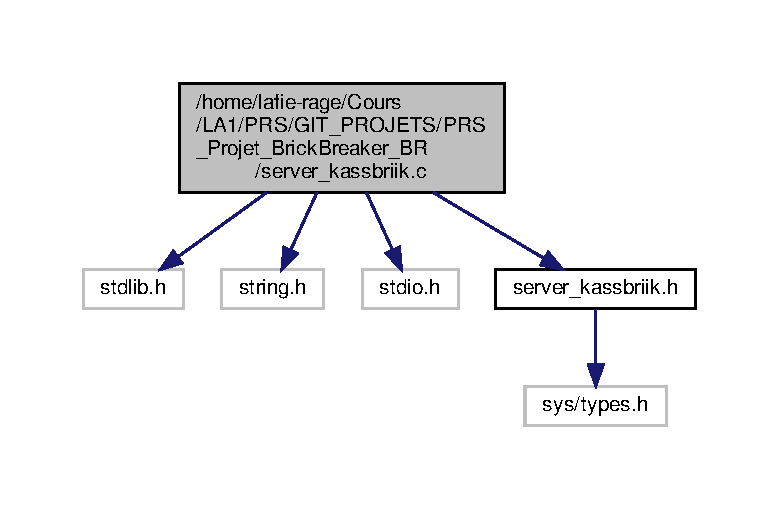
\includegraphics[width=350pt]{server__kassbriik_8c__incl}
\end{center}
\end{figure}
\subsection*{Functions}
\begin{DoxyCompactItemize}
\item 
void \hyperlink{server__kassbriik_8c_a28775a21a7c6ce6d81b13835bc0b7f38}{init\+Client\+List} (\hyperlink{server__kassbriik_8h_a0a2d0fa87306441ee5e7772d478fb8e4}{t\+\_\+clients\+\_\+list} $\ast$a, size\+\_\+t size)
\begin{DoxyCompactList}\small\item\em Initialise the t\+\_\+clients\+\_\+list structure. \end{DoxyCompactList}\item 
void \hyperlink{server__kassbriik_8c_a54f08f249535c5a9673652db9081dfe2}{remove\+Client\+From\+List} (\hyperlink{server__kassbriik_8h_a0a2d0fa87306441ee5e7772d478fb8e4}{t\+\_\+clients\+\_\+list} $\ast$a, int client\+Pid)
\item 
void \hyperlink{server__kassbriik_8c_ac42238b4d85d941aa8cbe94cebe6ef7a}{copy\+Clients\+List} (\hyperlink{server__kassbriik_8h_a0a2d0fa87306441ee5e7772d478fb8e4}{t\+\_\+clients\+\_\+list} $\ast$dest, \hyperlink{server__kassbriik_8h_a0a2d0fa87306441ee5e7772d478fb8e4}{t\+\_\+clients\+\_\+list} src)
\begin{DoxyCompactList}\small\item\em Copy a source list in the dest list. \end{DoxyCompactList}\item 
\hyperlink{structt__client}{t\+\_\+client} $\ast$ \hyperlink{server__kassbriik_8c_acf8de08461e2e2061e78628d95a5a053}{get\+Client\+By\+Pid} (\hyperlink{server__kassbriik_8h_a0a2d0fa87306441ee5e7772d478fb8e4}{t\+\_\+clients\+\_\+list} a, int client\+Pid)
\end{DoxyCompactItemize}


\subsection{Function Documentation}
\mbox{\Hypertarget{server__kassbriik_8c_ac42238b4d85d941aa8cbe94cebe6ef7a}\label{server__kassbriik_8c_ac42238b4d85d941aa8cbe94cebe6ef7a}} 
\index{server\+\_\+kassbriik.\+c@{server\+\_\+kassbriik.\+c}!copy\+Clients\+List@{copy\+Clients\+List}}
\index{copy\+Clients\+List@{copy\+Clients\+List}!server\+\_\+kassbriik.\+c@{server\+\_\+kassbriik.\+c}}
\subsubsection{\texorpdfstring{copy\+Clients\+List()}{copyClientsList()}}
{\footnotesize\ttfamily void copy\+Clients\+List (\begin{DoxyParamCaption}\item[{\hyperlink{server__kassbriik_8h_a0a2d0fa87306441ee5e7772d478fb8e4}{t\+\_\+clients\+\_\+list} $\ast$}]{dest,  }\item[{\hyperlink{server__kassbriik_8h_a0a2d0fa87306441ee5e7772d478fb8e4}{t\+\_\+clients\+\_\+list}}]{src }\end{DoxyParamCaption})}



Copy a source list in the dest list. 

Copy the src list in the dest preventing from accessing to the dest list when modifying the src list.


\begin{DoxyParams}{Parameters}
{\em dest} & The list in which the src will be copied. \\
\hline
{\em src} & The list that will be copied into the dest. \\
\hline
\end{DoxyParams}


Definition at line 40 of file server\+\_\+kassbriik.\+c.

\mbox{\Hypertarget{server__kassbriik_8c_acf8de08461e2e2061e78628d95a5a053}\label{server__kassbriik_8c_acf8de08461e2e2061e78628d95a5a053}} 
\index{server\+\_\+kassbriik.\+c@{server\+\_\+kassbriik.\+c}!get\+Client\+By\+Pid@{get\+Client\+By\+Pid}}
\index{get\+Client\+By\+Pid@{get\+Client\+By\+Pid}!server\+\_\+kassbriik.\+c@{server\+\_\+kassbriik.\+c}}
\subsubsection{\texorpdfstring{get\+Client\+By\+Pid()}{getClientByPid()}}
{\footnotesize\ttfamily \hyperlink{structt__client}{t\+\_\+client}$\ast$ get\+Client\+By\+Pid (\begin{DoxyParamCaption}\item[{\hyperlink{server__kassbriik_8h_a0a2d0fa87306441ee5e7772d478fb8e4}{t\+\_\+clients\+\_\+list}}]{a,  }\item[{int}]{client\+Pid }\end{DoxyParamCaption})}



Definition at line 52 of file server\+\_\+kassbriik.\+c.

\mbox{\Hypertarget{server__kassbriik_8c_a28775a21a7c6ce6d81b13835bc0b7f38}\label{server__kassbriik_8c_a28775a21a7c6ce6d81b13835bc0b7f38}} 
\index{server\+\_\+kassbriik.\+c@{server\+\_\+kassbriik.\+c}!init\+Client\+List@{init\+Client\+List}}
\index{init\+Client\+List@{init\+Client\+List}!server\+\_\+kassbriik.\+c@{server\+\_\+kassbriik.\+c}}
\subsubsection{\texorpdfstring{init\+Client\+List()}{initClientList()}}
{\footnotesize\ttfamily void init\+Client\+List (\begin{DoxyParamCaption}\item[{\hyperlink{server__kassbriik_8h_a0a2d0fa87306441ee5e7772d478fb8e4}{t\+\_\+clients\+\_\+list} $\ast$}]{a,  }\item[{size\+\_\+t}]{size }\end{DoxyParamCaption})}



Initialise the t\+\_\+clients\+\_\+list structure. 

/file \hyperlink{server__kassbriik_8c}{server\+\_\+kassbriik.\+c} /author Corentin D\+E\+S\+T\+R\+EZ \& Valentin G\+U\+I\+B\+E\+R\+T\+E\+AU /date 09 Apr 2021 /brief Source code of the server\textquotesingle{}s library

This library containts the definition of some useful values, functions and structures that are used by the server.

Initialise the send structure depending on the send size. This function will set up the size of the list and initialise every value of the array to -\/1 as default value.


\begin{DoxyParams}{Parameters}
{\em a} & The t\+\_\+clients\+\_\+list to initialise. \\
\hline
{\em size} & The size of the list. \\
\hline
\end{DoxyParams}


Definition at line 21 of file server\+\_\+kassbriik.\+c.

\mbox{\Hypertarget{server__kassbriik_8c_a54f08f249535c5a9673652db9081dfe2}\label{server__kassbriik_8c_a54f08f249535c5a9673652db9081dfe2}} 
\index{server\+\_\+kassbriik.\+c@{server\+\_\+kassbriik.\+c}!remove\+Client\+From\+List@{remove\+Client\+From\+List}}
\index{remove\+Client\+From\+List@{remove\+Client\+From\+List}!server\+\_\+kassbriik.\+c@{server\+\_\+kassbriik.\+c}}
\subsubsection{\texorpdfstring{remove\+Client\+From\+List()}{removeClientFromList()}}
{\footnotesize\ttfamily void remove\+Client\+From\+List (\begin{DoxyParamCaption}\item[{\hyperlink{server__kassbriik_8h_a0a2d0fa87306441ee5e7772d478fb8e4}{t\+\_\+clients\+\_\+list} $\ast$}]{a,  }\item[{int}]{client\+Pid }\end{DoxyParamCaption})}



Definition at line 29 of file server\+\_\+kassbriik.\+c.


\hypertarget{server__kassbriik_8h}{}\section{/home/lafie-\/rage/\+Cours/\+L\+A1/\+P\+R\+S/\+G\+I\+T\+\_\+\+P\+R\+O\+J\+E\+T\+S/\+P\+R\+S\+\_\+\+Projet\+\_\+\+Brick\+Breaker\+\_\+\+B\+R/server\+\_\+kassbriik.h File Reference}
\label{server__kassbriik_8h}\index{/home/lafie-\/rage/\+Cours/\+L\+A1/\+P\+R\+S/\+G\+I\+T\+\_\+\+P\+R\+O\+J\+E\+T\+S/\+P\+R\+S\+\_\+\+Projet\+\_\+\+Brick\+Breaker\+\_\+\+B\+R/server\+\_\+kassbriik.\+h@{/home/lafie-\/rage/\+Cours/\+L\+A1/\+P\+R\+S/\+G\+I\+T\+\_\+\+P\+R\+O\+J\+E\+T\+S/\+P\+R\+S\+\_\+\+Projet\+\_\+\+Brick\+Breaker\+\_\+\+B\+R/server\+\_\+kassbriik.\+h}}
{\ttfamily \#include $<$sys/types.\+h$>$}\newline
Include dependency graph for server\+\_\+kassbriik.\+h\+:\nopagebreak
\begin{figure}[H]
\begin{center}
\leavevmode
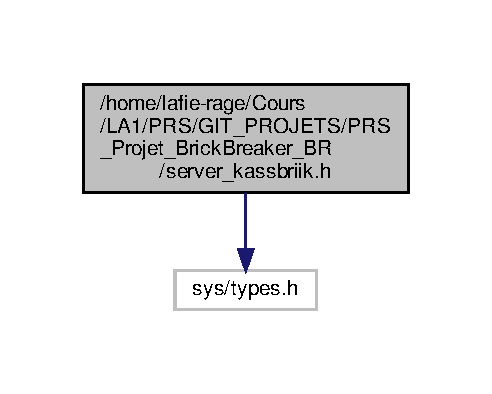
\includegraphics[width=236pt]{server__kassbriik_8h__incl}
\end{center}
\end{figure}
This graph shows which files directly or indirectly include this file\+:\nopagebreak
\begin{figure}[H]
\begin{center}
\leavevmode
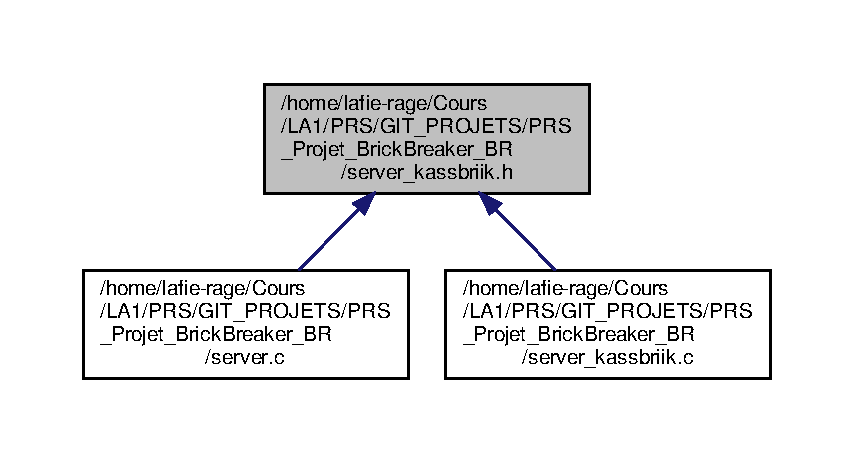
\includegraphics[width=350pt]{server__kassbriik_8h__dep__incl}
\end{center}
\end{figure}
\subsection*{Data Structures}
\begin{DoxyCompactItemize}
\item 
struct \hyperlink{structclient}{client}
\item 
struct \hyperlink{structclients__list}{clients\+\_\+list}
\begin{DoxyCompactList}\small\item\em A list of clients. \end{DoxyCompactList}\end{DoxyCompactItemize}
\subsection*{Typedefs}
\begin{DoxyCompactItemize}
\item 
typedef struct \hyperlink{structclient}{client} \hyperlink{server__kassbriik_8h_ab703f4f76628473adcf9246202352fe9}{t\+\_\+client}
\item 
typedef struct \hyperlink{structclients__list}{clients\+\_\+list} \hyperlink{server__kassbriik_8h_a0a2d0fa87306441ee5e7772d478fb8e4}{t\+\_\+clients\+\_\+list}
\end{DoxyCompactItemize}
\subsection*{Functions}
\begin{DoxyCompactItemize}
\item 
void \hyperlink{server__kassbriik_8h_a28775a21a7c6ce6d81b13835bc0b7f38}{init\+Client\+List} (\hyperlink{server__kassbriik_8h_a0a2d0fa87306441ee5e7772d478fb8e4}{t\+\_\+clients\+\_\+list} $\ast$a, size\+\_\+t size)
\begin{DoxyCompactList}\small\item\em Initialise the t\+\_\+clients\+\_\+list structure. \end{DoxyCompactList}\item 
void \hyperlink{server__kassbriik_8h_a54f08f249535c5a9673652db9081dfe2}{remove\+Client\+From\+List} (\hyperlink{server__kassbriik_8h_a0a2d0fa87306441ee5e7772d478fb8e4}{t\+\_\+clients\+\_\+list} $\ast$a, int client\+Pid)
\item 
void \hyperlink{server__kassbriik_8h_ac42238b4d85d941aa8cbe94cebe6ef7a}{copy\+Clients\+List} (\hyperlink{server__kassbriik_8h_a0a2d0fa87306441ee5e7772d478fb8e4}{t\+\_\+clients\+\_\+list} $\ast$dest, \hyperlink{server__kassbriik_8h_a0a2d0fa87306441ee5e7772d478fb8e4}{t\+\_\+clients\+\_\+list} src)
\begin{DoxyCompactList}\small\item\em Copy a source list in the dest list. \end{DoxyCompactList}\item 
\hyperlink{structt__client}{t\+\_\+client} $\ast$ \hyperlink{server__kassbriik_8h_acf8de08461e2e2061e78628d95a5a053}{get\+Client\+By\+Pid} (\hyperlink{server__kassbriik_8h_a0a2d0fa87306441ee5e7772d478fb8e4}{t\+\_\+clients\+\_\+list} a, int client\+Pid)
\end{DoxyCompactItemize}


\subsection{Typedef Documentation}
\mbox{\Hypertarget{server__kassbriik_8h_ab703f4f76628473adcf9246202352fe9}\label{server__kassbriik_8h_ab703f4f76628473adcf9246202352fe9}} 
\index{server\+\_\+kassbriik.\+h@{server\+\_\+kassbriik.\+h}!t\+\_\+client@{t\+\_\+client}}
\index{t\+\_\+client@{t\+\_\+client}!server\+\_\+kassbriik.\+h@{server\+\_\+kassbriik.\+h}}
\subsubsection{\texorpdfstring{t\+\_\+client}{t\_client}}
{\footnotesize\ttfamily typedef struct \hyperlink{structclient}{client}  \hyperlink{structt__client}{t\+\_\+client}}

\mbox{\Hypertarget{server__kassbriik_8h_a0a2d0fa87306441ee5e7772d478fb8e4}\label{server__kassbriik_8h_a0a2d0fa87306441ee5e7772d478fb8e4}} 
\index{server\+\_\+kassbriik.\+h@{server\+\_\+kassbriik.\+h}!t\+\_\+clients\+\_\+list@{t\+\_\+clients\+\_\+list}}
\index{t\+\_\+clients\+\_\+list@{t\+\_\+clients\+\_\+list}!server\+\_\+kassbriik.\+h@{server\+\_\+kassbriik.\+h}}
\subsubsection{\texorpdfstring{t\+\_\+clients\+\_\+list}{t\_clients\_list}}
{\footnotesize\ttfamily typedef struct \hyperlink{structclients__list}{clients\+\_\+list}  \hyperlink{server__kassbriik_8h_a0a2d0fa87306441ee5e7772d478fb8e4}{t\+\_\+clients\+\_\+list}}



\subsection{Function Documentation}
\mbox{\Hypertarget{server__kassbriik_8h_ac42238b4d85d941aa8cbe94cebe6ef7a}\label{server__kassbriik_8h_ac42238b4d85d941aa8cbe94cebe6ef7a}} 
\index{server\+\_\+kassbriik.\+h@{server\+\_\+kassbriik.\+h}!copy\+Clients\+List@{copy\+Clients\+List}}
\index{copy\+Clients\+List@{copy\+Clients\+List}!server\+\_\+kassbriik.\+h@{server\+\_\+kassbriik.\+h}}
\subsubsection{\texorpdfstring{copy\+Clients\+List()}{copyClientsList()}}
{\footnotesize\ttfamily void copy\+Clients\+List (\begin{DoxyParamCaption}\item[{\hyperlink{server__kassbriik_8h_a0a2d0fa87306441ee5e7772d478fb8e4}{t\+\_\+clients\+\_\+list} $\ast$}]{dest,  }\item[{\hyperlink{server__kassbriik_8h_a0a2d0fa87306441ee5e7772d478fb8e4}{t\+\_\+clients\+\_\+list}}]{src }\end{DoxyParamCaption})}



Copy a source list in the dest list. 

Copy the src list in the dest preventing from accessing to the dest list when modifying the src list.


\begin{DoxyParams}{Parameters}
{\em dest} & The list in which the src will be copied. \\
\hline
{\em src} & The list that will be copied into the dest. \\
\hline
\end{DoxyParams}


Definition at line 40 of file server\+\_\+kassbriik.\+c.

\mbox{\Hypertarget{server__kassbriik_8h_acf8de08461e2e2061e78628d95a5a053}\label{server__kassbriik_8h_acf8de08461e2e2061e78628d95a5a053}} 
\index{server\+\_\+kassbriik.\+h@{server\+\_\+kassbriik.\+h}!get\+Client\+By\+Pid@{get\+Client\+By\+Pid}}
\index{get\+Client\+By\+Pid@{get\+Client\+By\+Pid}!server\+\_\+kassbriik.\+h@{server\+\_\+kassbriik.\+h}}
\subsubsection{\texorpdfstring{get\+Client\+By\+Pid()}{getClientByPid()}}
{\footnotesize\ttfamily \hyperlink{structt__client}{t\+\_\+client}$\ast$ get\+Client\+By\+Pid (\begin{DoxyParamCaption}\item[{\hyperlink{server__kassbriik_8h_a0a2d0fa87306441ee5e7772d478fb8e4}{t\+\_\+clients\+\_\+list}}]{a,  }\item[{int}]{client\+Pid }\end{DoxyParamCaption})}



Definition at line 52 of file server\+\_\+kassbriik.\+c.

\mbox{\Hypertarget{server__kassbriik_8h_a28775a21a7c6ce6d81b13835bc0b7f38}\label{server__kassbriik_8h_a28775a21a7c6ce6d81b13835bc0b7f38}} 
\index{server\+\_\+kassbriik.\+h@{server\+\_\+kassbriik.\+h}!init\+Client\+List@{init\+Client\+List}}
\index{init\+Client\+List@{init\+Client\+List}!server\+\_\+kassbriik.\+h@{server\+\_\+kassbriik.\+h}}
\subsubsection{\texorpdfstring{init\+Client\+List()}{initClientList()}}
{\footnotesize\ttfamily void init\+Client\+List (\begin{DoxyParamCaption}\item[{\hyperlink{server__kassbriik_8h_a0a2d0fa87306441ee5e7772d478fb8e4}{t\+\_\+clients\+\_\+list} $\ast$}]{a,  }\item[{size\+\_\+t}]{size }\end{DoxyParamCaption})}



Initialise the t\+\_\+clients\+\_\+list structure. 

/file \hyperlink{server__kassbriik_8c}{server\+\_\+kassbriik.\+c} /author Corentin D\+E\+S\+T\+R\+EZ \& Valentin G\+U\+I\+B\+E\+R\+T\+E\+AU /date 09 Apr 2021 /brief Source code of the server\textquotesingle{}s library

This library containts the definition of some useful values, functions and structures that are used by the server.

Initialise the send structure depending on the send size. This function will set up the size of the list and initialise every value of the array to -\/1 as default value.


\begin{DoxyParams}{Parameters}
{\em a} & The t\+\_\+clients\+\_\+list to initialise. \\
\hline
{\em size} & The size of the list. \\
\hline
\end{DoxyParams}


Definition at line 21 of file server\+\_\+kassbriik.\+c.

\mbox{\Hypertarget{server__kassbriik_8h_a54f08f249535c5a9673652db9081dfe2}\label{server__kassbriik_8h_a54f08f249535c5a9673652db9081dfe2}} 
\index{server\+\_\+kassbriik.\+h@{server\+\_\+kassbriik.\+h}!remove\+Client\+From\+List@{remove\+Client\+From\+List}}
\index{remove\+Client\+From\+List@{remove\+Client\+From\+List}!server\+\_\+kassbriik.\+h@{server\+\_\+kassbriik.\+h}}
\subsubsection{\texorpdfstring{remove\+Client\+From\+List()}{removeClientFromList()}}
{\footnotesize\ttfamily void remove\+Client\+From\+List (\begin{DoxyParamCaption}\item[{\hyperlink{server__kassbriik_8h_a0a2d0fa87306441ee5e7772d478fb8e4}{t\+\_\+clients\+\_\+list} $\ast$}]{a,  }\item[{int}]{client\+Pid }\end{DoxyParamCaption})}



Definition at line 29 of file server\+\_\+kassbriik.\+c.


%--- End generated contents ---

% Index
\backmatter
\newpage
\phantomsection
\clearemptydoublepage
\addcontentsline{toc}{chapter}{Index}
\printindex

\end{document}
